% Options for packages loaded elsewhere
\PassOptionsToPackage{unicode}{hyperref}
\PassOptionsToPackage{hyphens}{url}
%
\documentclass[
]{book}
\usepackage{amsmath,amssymb}
\usepackage{lmodern}
\usepackage{ifxetex,ifluatex}
\ifnum 0\ifxetex 1\fi\ifluatex 1\fi=0 % if pdftex
  \usepackage[T1]{fontenc}
  \usepackage[utf8]{inputenc}
  \usepackage{textcomp} % provide euro and other symbols
\else % if luatex or xetex
  \usepackage{unicode-math}
  \defaultfontfeatures{Scale=MatchLowercase}
  \defaultfontfeatures[\rmfamily]{Ligatures=TeX,Scale=1}
\fi
% Use upquote if available, for straight quotes in verbatim environments
\IfFileExists{upquote.sty}{\usepackage{upquote}}{}
\IfFileExists{microtype.sty}{% use microtype if available
  \usepackage[]{microtype}
  \UseMicrotypeSet[protrusion]{basicmath} % disable protrusion for tt fonts
}{}
\makeatletter
\@ifundefined{KOMAClassName}{% if non-KOMA class
  \IfFileExists{parskip.sty}{%
    \usepackage{parskip}
  }{% else
    \setlength{\parindent}{0pt}
    \setlength{\parskip}{6pt plus 2pt minus 1pt}}
}{% if KOMA class
  \KOMAoptions{parskip=half}}
\makeatother
\usepackage{xcolor}
\IfFileExists{xurl.sty}{\usepackage{xurl}}{} % add URL line breaks if available
\IfFileExists{bookmark.sty}{\usepackage{bookmark}}{\usepackage{hyperref}}
\hypersetup{
  pdftitle={STAT 234: Data Science},
  pdfauthor={Matt Higham},
  hidelinks,
  pdfcreator={LaTeX via pandoc}}
\urlstyle{same} % disable monospaced font for URLs
\usepackage{color}
\usepackage{fancyvrb}
\newcommand{\VerbBar}{|}
\newcommand{\VERB}{\Verb[commandchars=\\\{\}]}
\DefineVerbatimEnvironment{Highlighting}{Verbatim}{commandchars=\\\{\}}
% Add ',fontsize=\small' for more characters per line
\usepackage{framed}
\definecolor{shadecolor}{RGB}{248,248,248}
\newenvironment{Shaded}{\begin{snugshade}}{\end{snugshade}}
\newcommand{\AlertTok}[1]{\textcolor[rgb]{0.94,0.16,0.16}{#1}}
\newcommand{\AnnotationTok}[1]{\textcolor[rgb]{0.56,0.35,0.01}{\textbf{\textit{#1}}}}
\newcommand{\AttributeTok}[1]{\textcolor[rgb]{0.77,0.63,0.00}{#1}}
\newcommand{\BaseNTok}[1]{\textcolor[rgb]{0.00,0.00,0.81}{#1}}
\newcommand{\BuiltInTok}[1]{#1}
\newcommand{\CharTok}[1]{\textcolor[rgb]{0.31,0.60,0.02}{#1}}
\newcommand{\CommentTok}[1]{\textcolor[rgb]{0.56,0.35,0.01}{\textit{#1}}}
\newcommand{\CommentVarTok}[1]{\textcolor[rgb]{0.56,0.35,0.01}{\textbf{\textit{#1}}}}
\newcommand{\ConstantTok}[1]{\textcolor[rgb]{0.00,0.00,0.00}{#1}}
\newcommand{\ControlFlowTok}[1]{\textcolor[rgb]{0.13,0.29,0.53}{\textbf{#1}}}
\newcommand{\DataTypeTok}[1]{\textcolor[rgb]{0.13,0.29,0.53}{#1}}
\newcommand{\DecValTok}[1]{\textcolor[rgb]{0.00,0.00,0.81}{#1}}
\newcommand{\DocumentationTok}[1]{\textcolor[rgb]{0.56,0.35,0.01}{\textbf{\textit{#1}}}}
\newcommand{\ErrorTok}[1]{\textcolor[rgb]{0.64,0.00,0.00}{\textbf{#1}}}
\newcommand{\ExtensionTok}[1]{#1}
\newcommand{\FloatTok}[1]{\textcolor[rgb]{0.00,0.00,0.81}{#1}}
\newcommand{\FunctionTok}[1]{\textcolor[rgb]{0.00,0.00,0.00}{#1}}
\newcommand{\ImportTok}[1]{#1}
\newcommand{\InformationTok}[1]{\textcolor[rgb]{0.56,0.35,0.01}{\textbf{\textit{#1}}}}
\newcommand{\KeywordTok}[1]{\textcolor[rgb]{0.13,0.29,0.53}{\textbf{#1}}}
\newcommand{\NormalTok}[1]{#1}
\newcommand{\OperatorTok}[1]{\textcolor[rgb]{0.81,0.36,0.00}{\textbf{#1}}}
\newcommand{\OtherTok}[1]{\textcolor[rgb]{0.56,0.35,0.01}{#1}}
\newcommand{\PreprocessorTok}[1]{\textcolor[rgb]{0.56,0.35,0.01}{\textit{#1}}}
\newcommand{\RegionMarkerTok}[1]{#1}
\newcommand{\SpecialCharTok}[1]{\textcolor[rgb]{0.00,0.00,0.00}{#1}}
\newcommand{\SpecialStringTok}[1]{\textcolor[rgb]{0.31,0.60,0.02}{#1}}
\newcommand{\StringTok}[1]{\textcolor[rgb]{0.31,0.60,0.02}{#1}}
\newcommand{\VariableTok}[1]{\textcolor[rgb]{0.00,0.00,0.00}{#1}}
\newcommand{\VerbatimStringTok}[1]{\textcolor[rgb]{0.31,0.60,0.02}{#1}}
\newcommand{\WarningTok}[1]{\textcolor[rgb]{0.56,0.35,0.01}{\textbf{\textit{#1}}}}
\usepackage{longtable,booktabs,array}
\usepackage{calc} % for calculating minipage widths
% Correct order of tables after \paragraph or \subparagraph
\usepackage{etoolbox}
\makeatletter
\patchcmd\longtable{\par}{\if@noskipsec\mbox{}\fi\par}{}{}
\makeatother
% Allow footnotes in longtable head/foot
\IfFileExists{footnotehyper.sty}{\usepackage{footnotehyper}}{\usepackage{footnote}}
\makesavenoteenv{longtable}
\usepackage{graphicx}
\makeatletter
\def\maxwidth{\ifdim\Gin@nat@width>\linewidth\linewidth\else\Gin@nat@width\fi}
\def\maxheight{\ifdim\Gin@nat@height>\textheight\textheight\else\Gin@nat@height\fi}
\makeatother
% Scale images if necessary, so that they will not overflow the page
% margins by default, and it is still possible to overwrite the defaults
% using explicit options in \includegraphics[width, height, ...]{}
\setkeys{Gin}{width=\maxwidth,height=\maxheight,keepaspectratio}
% Set default figure placement to htbp
\makeatletter
\def\fps@figure{htbp}
\makeatother
\setlength{\emergencystretch}{3em} % prevent overfull lines
\providecommand{\tightlist}{%
  \setlength{\itemsep}{0pt}\setlength{\parskip}{0pt}}
\setcounter{secnumdepth}{5}
\usepackage{booktabs}
\ifluatex
  \usepackage{selnolig}  % disable illegal ligatures
\fi
\usepackage[]{natbib}
\bibliographystyle{apalike}

\title{STAT 234: Data Science}
\author{Matt Higham}
\date{2021-08-09}

\begin{document}
\maketitle

{
\setcounter{tocdepth}{1}
\tableofcontents
}
\hypertarget{syllabus-and-course-information}{%
\chapter{Syllabus and Course Information}\label{syllabus-and-course-information}}

\hypertarget{general-information}{%
\section{General Information}\label{general-information}}

\textbf{Instructor Information}

\begin{itemize}
\tightlist
\item
  Professor: Matt Higham
\item
  Office: Bewkes 123
\item
  Email: \href{mailto:mhigham@stlawu.edu}{\nolinkurl{mhigham@stlawu.edu}}
\item
  Semester: Fall 2021
\item
  Office Hours:

  \begin{itemize}
  \tightlist
  \item
    Tuesday 1:30 - 3:30
  \item
    Wednesday 2:30 - 3:30
  \item
    Friday 10:00 - 11:00
  \item
    other times by appointment
  \item
    all in-person
  \end{itemize}
\item
  Sections:

  \begin{itemize}
  \tightlist
  \item
    MW 8:50 - 10:20
  \end{itemize}
\end{itemize}

\textbf{Course Materials}

\begin{itemize}
\tightlist
\item
  STAT 234 Materials Bundle. This will be our primary source of materials.
\item
  Textbooks (only used as references):

  \begin{itemize}
  \tightlist
  \item
    Modern Data Science with \texttt{R} by Baumer, Kaplan, and Horton, found here in a free online version.
  \item
    R for Data Science by Grolemund and Wickham, found here in a free online version.
  \end{itemize}
\item
  Computer with Internet access.
\end{itemize}

\begin{center}\rule{0.5\linewidth}{0.5pt}\end{center}

\begin{center}\rule{0.5\linewidth}{0.5pt}\end{center}

\hypertarget{course-information}{%
\section{Course Information}\label{course-information}}

Welcome to STAT 234! The overall purpose of this course is learn the data science skills necessary to complete large-scale data analysis projects. The tool that we will be using to achieve this goal is the statistical software language \texttt{R}. We will work with a wide variety of interesting data sets throughout the semester to build our \texttt{R} skills. In particular, we will focus on the Data Analysis Life Cycle (Grolemund and Wickham 2020):

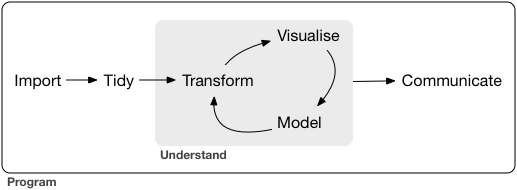
\includegraphics{other/data-science.png}

We will put more emphasis on the \emph{Import, Tidy, Transform, Visualize, and Communicate} parts of the cycle, as an introduction to \emph{Modeling} part is covered in STAT 213.

\begin{center}\rule{0.5\linewidth}{0.5pt}\end{center}

\begin{center}\rule{0.5\linewidth}{0.5pt}\end{center}

\hypertarget{general-course-outcomes}{%
\section{General Course Outcomes}\label{general-course-outcomes}}

\begin{enumerate}
\def\labelenumi{\arabic{enumi}.}
\item
  \emph{Import} data of a few different types into \texttt{R} for analysis.
\item
  \emph{Tidy} data into a form that can be more easily visualized, summarised, and modeled.
\item
  \emph{Transform}, \emph{Wrangle}, and \emph{Visualize} variables in a data set to assess patterns in the data.
\item
  \emph{Communicate} the results of your analysis to a target audience with a written report, or, possibly an oral presentation.
\item
  Practice reproducible statistical practices through the use of \texttt{R\ Markdown} for data analysis projects.
\item
  Explain why it is ethically important to consider the context that a data set comes in.
\item
  Develop the necessary skills to be able to ask and answer future data analysis questions on your own, either using \texttt{R} or another program, such as Python.
\end{enumerate}

To paraphrase the \emph{R for Data Science} textbook, about 80\% of the skills necessary to do a complete data analysis project can be learned through coursework in classes like this one. But, 20\% of any particular project will involve learning new things that are specific to that project. Achieving Goal \# 6 will allow you to learn this extra 20\% on your own.

\hypertarget{use-of-r-and-rstudio}{%
\subsection{\texorpdfstring{Use of \texttt{R} and \texttt{RStudio}}{Use of R and RStudio}}\label{use-of-r-and-rstudio}}

We will use the statistical software \texttt{R} to construct graphs and analyze data. A few notes:

\begin{itemize}
\tightlist
\item
  \texttt{R} and \texttt{RStudio} are both free to use.
\item
  We will primarily be using the SLU \texttt{R\ Studio} server at first: Link to R Studio Server.
\item
  Additionally, we will be using \texttt{RMarkdown} for data analysis reports.
  \emph{Note}: It's always nice to start assignments and projects as early as possible, but this is particularly important to do for assignments and projects involving \texttt{R}. It's no fun to try and figure out why code is not working at the last minute. If you start early enough though, you will have plenty of time to seek help and therefore won't waste a lot of time on a coding error.
\end{itemize}

\begin{center}\rule{0.5\linewidth}{0.5pt}\end{center}

\begin{center}\rule{0.5\linewidth}{0.5pt}\end{center}

\hypertarget{how-you-will-be-assessed}{%
\section{How You Will Be Assessed}\label{how-you-will-be-assessed}}

The components to your grade are described below:

\begin{itemize}
\tightlist
\item
  Class
\end{itemize}

Class participation will be assessed three times throughout the semester in a 20 point rubric for a total of 60 points. Additionally, there will be a 10-point ``share something interesting you found with the class'' assignment on very Wednesday, where, two students will volunteer to\ldots.share something interesting that they found with the data set we were working with with the rest of the class. The rubric used will be shared on the first day of class, and more information about the Wednesday 10 points will also be given on the first day of class.

\begin{itemize}
\tightlist
\item
  Exercises
\end{itemize}

There are about 14 sets of weekly exercises that often require you to read some of the sections in the STAT 234 Materials Bundle first. These are worth either 10 or 5 points, depending on the length of the exercises, for a total of 100 points. Most weeks toward the beginning of the semester will be 10 point weeks because we won't have any projects to work on. Exercises are graded \textbf{for completion only}: for many exercises, the solutions are provided in our course materials.

\begin{itemize}
\tightlist
\item
  Quizzes
\end{itemize}

There will be 10 Quizzes, each worth 20 points for a total of 180 points with one dropped quiz. The purpose of the quizzes are for you to practice what you've learned for the week in a short, concise format. Quizzes will consist of two parts: (1) a take-home component and (2) an in-class component. The take-home component should take about 15 minutes. You are allowed use any course materials and you are allowed to work with other students in this course, as long as you list the names of those students at the top of your quiz. The in-class component will be 5 minutes. You will be asked to do a simple task with pen and paper, without using any course notes or materials.

\begin{itemize}
\tightlist
\item
  Mini Projects
\end{itemize}

There are 3 mini-projects scattered throughout the semester that are worth 60 points each. Each mini-project will have some prescriptive tasks and questions that you will investigate as well as a section where you come up with and subsequently answer your own questions relating to the data set.

In order to get experience with oral presentations of results, each student will give a short oral presentation on \textbf{1} mini-project. Use of \texttt{R\ Markdown} is required for this presentation (as opposed to PowerPoint or Prezi). More details will be given later in the semester.

\begin{itemize}
\tightlist
\item
  Midterm Exams
\end{itemize}

There will be two midterm exams, each worth 150 points. More information will be given about these later.

\begin{itemize}
\tightlist
\item
  Final Project
\end{itemize}

There is one final project, worth 150 points. The primary purpose of the final project is to give you an opportunity to assemble topics throughout the course into one coherent data analysis. More information about the final project will be given later.

There will be no Final Exam for this course.

\hypertarget{breakdown}{%
\subsection{Breakdown}\label{breakdown}}

\begin{itemize}
\tightlist
\item
  70 points for Class
\item
  100 points for Exercises
\item
  180 points for Quizzes
\item
  180 points for Mini-Projects + 20 points for Presentation
\item
  150 points for each of two Midterm Exams
\item
  150 points for Final Project
\end{itemize}

Points add up to 1000 so your grade at the end of the semester will be the number of points you've earned across all categories divided by 1000.

\begin{itemize}
\tightlist
\item
  The tutorials should help you complete the exercises sets, which should

  \begin{itemize}
  \tightlist
  \item
    help you to do well on the quizzes, which should

    \begin{itemize}
    \tightlist
    \item
      help you complete the mini-projects, which should

      \begin{itemize}
      \tightlist
      \item
        help you to do well on the midterm exams.
      \end{itemize}
    \end{itemize}
  \end{itemize}
\end{itemize}

Then, everything together should help you create an awesome final project!

\hypertarget{grading-scale}{%
\subsection{Grading Scale}\label{grading-scale}}

The following is a \emph{rough} grading scale. I reserve the right to make any changes to the scale if necessary.

\begin{longtable}[]{@{}
  >{\raggedright\arraybackslash}p{(\columnwidth - 28\tabcolsep) * \real{0.07}}
  >{\raggedright\arraybackslash}p{(\columnwidth - 28\tabcolsep) * \real{0.07}}
  >{\raggedright\arraybackslash}p{(\columnwidth - 28\tabcolsep) * \real{0.07}}
  >{\raggedright\arraybackslash}p{(\columnwidth - 28\tabcolsep) * \real{0.07}}
  >{\raggedright\arraybackslash}p{(\columnwidth - 28\tabcolsep) * \real{0.07}}
  >{\raggedright\arraybackslash}p{(\columnwidth - 28\tabcolsep) * \real{0.07}}
  >{\raggedright\arraybackslash}p{(\columnwidth - 28\tabcolsep) * \real{0.07}}
  >{\raggedright\arraybackslash}p{(\columnwidth - 28\tabcolsep) * \real{0.07}}
  >{\raggedright\arraybackslash}p{(\columnwidth - 28\tabcolsep) * \real{0.07}}
  >{\raggedright\arraybackslash}p{(\columnwidth - 28\tabcolsep) * \real{0.07}}
  >{\raggedright\arraybackslash}p{(\columnwidth - 28\tabcolsep) * \real{0.07}}
  >{\raggedright\arraybackslash}p{(\columnwidth - 28\tabcolsep) * \real{0.07}}
  >{\raggedright\arraybackslash}p{(\columnwidth - 28\tabcolsep) * \real{0.07}}
  >{\raggedright\arraybackslash}p{(\columnwidth - 28\tabcolsep) * \real{0.07}}
  >{\raggedright\arraybackslash}p{(\columnwidth - 28\tabcolsep) * \real{0.07}}@{}}
\toprule
Grade & 4.0 & 3.75 & 3.5 & 3.25 & 3.0 & 2.75 & 2.5 & 2.25 & 2.0 & 1.75 & 1.5 & 1.25 & 1.0 & 0.0 \\
\midrule
\endhead
Points & 950-1000 & 920-949 & 890-919 & 860-889 & 830-859 & 810-829 & 770-809 & 750-769 & 720-749 & 700-719 & 670-699 & 640-669 & 600-639 & 0-599 \\
\bottomrule
\end{longtable}

\begin{center}\rule{0.5\linewidth}{0.5pt}\end{center}

\begin{center}\rule{0.5\linewidth}{0.5pt}\end{center}

\hypertarget{rules-for-collaboration}{%
\subsection{Rules for Collaboration}\label{rules-for-collaboration}}

Collaboration with your classmates on handouts, tutorials, and projects is encouraged, but you must follow these guidelines:

\begin{itemize}
\tightlist
\item
  you must state the name(s) of who you collaborated with at the top of each assessment.
\item
  all work must be your own. This means that you should \textbf{never} send someone your code via email or let someone directly type code off of your screen. Instead, you can talk about strategies for solving problems and help or ask someone about a coding error.
\item
  you may use the Internet and StackExchange, but you also should not copy paste code directly from the website, without citing that you did so.
\item
  this isn't a rule, but keep in mind that collaboration is not permitted on quizzes, exams, and very limited collaboration will be permitted on the final project. Therefore, when working with someone, make sure that you are both really learning so that you both can have success on the non-collaborative assessments.
\end{itemize}

\begin{center}\rule{0.5\linewidth}{0.5pt}\end{center}

\begin{center}\rule{0.5\linewidth}{0.5pt}\end{center}

\hypertarget{diversity-statement}{%
\subsection{Diversity Statement}\label{diversity-statement}}

Diversity encompasses differences in age, colour, ethnicity, national origin, gender, physical or mental ability, religion, socioeconomic background, veteran status, sexual orientation, and marginalized groups. The interaction of different human characteristics brings about a positive learning environment. Diversity is both respected and valued in this classroom.

\begin{center}\rule{0.5\linewidth}{0.5pt}\end{center}

\begin{center}\rule{0.5\linewidth}{0.5pt}\end{center}

\hypertarget{accessibility-statement}{%
\subsection{Accessibility Statement}\label{accessibility-statement}}

If you have a learning difference/disability or other health impairment and need accommodations please be sure to contact the Student Accessibility Services Office right away so they can help you get the accommodations you require. If you need to use any accommodations in this class, please meet with your instructor early and provide them with your Individualized Educational Accommodation Plan (IEAP) letter so you can have the best possible experience this semester.

Although not required, your instructor would like to know of any accommodations that are needed at least 10 days before a quiz or test. Please be proactive and set up an appointment to meet with someone from the Student Accessibility Services Office.

\textbf{Color-Vision Deficiency:} If you are Color-Vision Deficient, the Student Accessibility Services office has on loan glasses for students who are color vision deficient. Please contact the office to make an appointment.

For more specific information about setting up an appointment with Student Accessibility Services please see the listed options below:

\begin{itemize}
\tightlist
\item
  Telephone: 315.229.5537
\item
  Email: \href{mailto:studentaccessibility@stlawu.edu}{\nolinkurl{studentaccessibility@stlawu.edu}}
\end{itemize}

For further information about Student Accessibility Services you can check the website at: \url{https://www.stlawu.edu/student-accessibility-services}

\begin{center}\rule{0.5\linewidth}{0.5pt}\end{center}

\begin{center}\rule{0.5\linewidth}{0.5pt}\end{center}

\hypertarget{academic-dishonesty}{%
\subsection{Academic Dishonesty}\label{academic-dishonesty}}

Academic dishonesty will not be tolerated. Any specific policies for this course are supplementary to the

Honor Code. According to the St.~Lawrence University Academic Honor Policy,

\begin{enumerate}
\def\labelenumi{\arabic{enumi}.}
\tightlist
\item
  It is assumed that all work is done by the student unless the instructor/mentor/employer gives specific permission for collaboration.
\item
  Cheating on examinations and tests consists of knowingly giving or using or attempting to use unauthorized assistance during examinations or tests.
\item
  Dishonesty in work outside of examinations and tests consists of handing in or presenting as original work which is not original, where originality is required.
\end{enumerate}

\emph{Claims of ignorance and academic or personal pressure are unacceptable as excuses for academic dishonesty.} Students must learn what constitutes one's own work and how the work of others must be acknowledged.

For more information, refer to \href{../../C:\%5CUsers\%5Ciramler\%5CAppData\%5CLocal\%5CTemp\%5Cwww.stlawu.edu\%5Cacadaffairs\%5Cacademic_honor_policy.pdf}{www.stlawu.edu/acadaffairs/}\href{../../C:\%5CUsers\%5Ciramler\%5CAppData\%5CLocal\%5CTemp\%5Cwww.stlawu.edu\%5Cacadaffairs\%5Cacademic_honor_policy.pdf}{\textbf{academic}}\href{../../C:\%5CUsers\%5Ciramler\%5CAppData\%5CLocal\%5CTemp\%5Cwww.stlawu.edu\%5Cacadaffairs\%5Cacademic_honor_policy.pdf}{\_}\href{../../C:\%5CUsers\%5Ciramler\%5CAppData\%5CLocal\%5CTemp\%5Cwww.stlawu.edu\%5Cacadaffairs\%5Cacademic_honor_policy.pdf}{\textbf{honor}}\href{../../C:\%5CUsers\%5Ciramler\%5CAppData\%5CLocal\%5CTemp\%5Cwww.stlawu.edu\%5Cacadaffairs\%5Cacademic_honor_policy.pdf}{\_policy.pdf}.

To avoid academic dishonesty, it is important that you follow all directions and collaboration rules and ask for clarification if you have any questions about what is acceptable for a particular assignment or exam. If I suspect academic dishonesty, a score of zero will be given for the entire assignment in which the academic dishonesty occurred \textbf{for all individuals involved} and Academic Honor Council will be notified. If a pattern of academic dishonesty is found to have occurred, a grade of 0.0 for the entire course can be given.

It is important to work in a way that maximizes your learning. Be aware that students who rely too much on others for the homework and projects tend to do poorly on the quizzes and exams.

\emph{Please note that in addition the above, any assignments in which your score is reduced due to academic dishonesty will not be dropped according to the quiz policy e.g., if you receive a zero on a quiz because of academic dishonesty, it will not be dropped from your grade.}

\begin{center}\rule{0.5\linewidth}{0.5pt}\end{center}

\begin{center}\rule{0.5\linewidth}{0.5pt}\end{center}

\hypertarget{tentative-schedule}{%
\section{Tentative Schedule}\label{tentative-schedule}}

\begin{longtable}[]{@{}llll@{}}
\toprule
Week & Date & Topics & \\
\midrule
\endhead
0 & 8/25 & Introduction to \texttt{R}, \texttt{R\ Studio} & \\
1 & 8/30 & Graphics with \texttt{ggplot2} & \\
2 & 9/6 & Data Wrangling and Transformation with \texttt{dplyr} & \\
3 & 9/13 & Data Tidying with \texttt{tidyr} & \\
4 & 9/20 & Communication with \texttt{R\ Markdown} and \texttt{ggplot2} & \\
5 & 9/27 & Basic Coding in \texttt{R} & \\
6 & 10/4 & Catch-up and Midterm 1 & \\
& & & \\
7 & 10/11 & Factors with \texttt{forcats} and Data Ethics & \\
8 & 10/18 & Data Import with \texttt{readr}, \texttt{jsonlite}, \texttt{rvest}, and \texttt{tibble} & \\
9 & 10/25 & Data Merging with \texttt{dplyr} & \\
10 & 11/1 & Dates and Times with \texttt{lubridate} & \\
11 & 11/8 & Strings with \texttt{stringr} & \\
12 & 11/15 & Catch-up and Midterm 2 & \\
& & & \\
13 & 11/22 & Thanksgiving Break & \\
14 & 11/29 & Predictive Modeling Final Project & \\
14 & 12/6 & Final Project & \\
\bottomrule
\end{longtable}

\begin{itemize}
\tightlist
\item
  The three mini-projects are tentatively scheduled to be due on September 27, October 25, and November 8, though these are subject to change.
\item
  There will be no Final Exam, but keep your schedule open at our Final Exam time in case we decide to use it for something.
\end{itemize}

\hypertarget{intro}{%
\chapter{\texorpdfstring{Getting Started with \texttt{R} and \texttt{R\ Studio}}{Getting Started with R and R Studio}}\label{intro}}

\textbf{Goals}:

\begin{enumerate}
\def\labelenumi{\arabic{enumi}.}
\item
  Use \texttt{R\ Studio} on the server
\item
  Use \texttt{R\ Markdown} and code chunks
\item
  Load in data to \texttt{R\ Studio}
\item
  Run code and change a few things within that code
\item
  Correct some common errors when running code in \texttt{R}
\end{enumerate}

\hypertarget{intro-to-r-and-r-studio}{%
\section{\texorpdfstring{Intro to \texttt{R} and \texttt{R\ Studio}}{Intro to R and R Studio}}\label{intro-to-r-and-r-studio}}

\texttt{R} is a statistical computing software used by many statisticians as well as professionals in other fields, such as biology, ecology, business, and psychology. The goal of Week 0 is to provide basic familiarity with \texttt{R} and \texttt{R\ Markdown}, which we will be using for the entire semester.

Open \texttt{R\ Studio} on the SLU \texttt{R\ Studio} server at
http://rstudio.stlawu.local:8787 and create a folder called STAT\_234 or some other meaningful title to you. Note that you must be on campus to use the \texttt{R\ Studio} server, unless you use a VPN. Directions on how to set-up VPN are
https://infotech.stlawu.edu/support/content/11269
\textless\textgreater{} for Macs and https://stlawu.teamdynamix.com/TDClient/1805/Portal/KB/ArticleDet?ID=55118 for Windows.

Next, create a subfolder within your STAT\_234 folder. Title it \emph{Notes} (or whatever you want really).

Then, create an \texttt{R\ Project} by Clicking File -\textgreater{} New Project -\textgreater{} Existing Directory, navigate to the \emph{Notes} folder, and click \emph{Create Project}.

Within this folder, click the \emph{New Folder} button in your bottom-left window and name a new folder \emph{data}. Then, download the data.zip file from Sakai (in Resources). Upload that file in to the server by clicking ``Upload'' in the bottom right panel. In the dialog box that appears, you can click ``Choose File'' and navigate to the folder where you saved the zip file (probably Downloads by default). The zip file will automatically expand once uploaded. It includes data sets that we will use throughout the course.

Finally, we want to create a new \texttt{R\ Markdown} file by clicking File -\textgreater{} New File -\textgreater{} \texttt{R\ Markdown}. You can give your new \texttt{R\ Markdown} file a title if you want, and then click okay.

Before moving on, click the \textbf{Knit} button in the top-left window at the top of the menu bar (look for the knitting needle icon). Make sure that the file knits to a pretty-looking .html file. The newly knitted .html file can now be found in your folder with your \texttt{R} project.

\hypertarget{what-are-r-r-studio-and-r-markdown}{%
\section{\texorpdfstring{What are \texttt{R}, \texttt{R\ Studio}, and \texttt{R\ Markdown}?}{What are R, R Studio, and R Markdown?}}\label{what-are-r-r-studio-and-r-markdown}}

The distinction between the 3 will become more clear later on. For now,
* \texttt{R} is a statistical coding software used heavily for data analysis and statistical procedures.

\begin{itemize}
\item
  \texttt{R\ Studio} is a nice IDE (Integrated Development Environment) for \texttt{R} that has a lot of convenient features. Think of this as just a convenient User Interface.
\item
  \texttt{R\ Mardkown} allows users to mix regular Microsoft-Word-style text with code. The \texttt{.Rmd} file ending denotes an \texttt{R\ Mardkown} file. \texttt{R\ Markdown} has many options that we will use heavily throughout the semester, but there's no need to worry about these now.
\end{itemize}

\hypertarget{r-packages-and-the-tidyverse}{%
\subsection{\texorpdfstring{\texttt{R} Packages and the \texttt{tidyverse}}{R Packages and the tidyverse}}\label{r-packages-and-the-tidyverse}}

You can think of \texttt{R} packages as add-ons to \texttt{R} that let you do things that \texttt{R} on its own would not be able to do. If you're in to video games, you can think of \texttt{R} packages as extra Downloadable Content (DLC). But, unlike most gaming DLC, \texttt{R} packages are always free and we will make very heavy use of \texttt{R} packages.

The \texttt{tidyverse} is a series of \texttt{R} packages that are useful for data science. In the order that we will encounter them in this class, the core \texttt{tidyverse} packages are:

\begin{enumerate}
\def\labelenumi{\arabic{enumi}.}
\tightlist
\item
  \texttt{ggplot2} for plotting data
\item
  \texttt{dplyr} for data wrangling and summarizing
\item
  \texttt{tidyr} for data tidying and reshaping
\item
  \texttt{readr} for data import
\item
  \texttt{tibble} for how data is stored
\item
  \texttt{stringr} for text data
\item
  \texttt{forcats} for factor (categorical) data
\item
  \texttt{purrr}, for functional programming, the only one of these core 8 that we won't get to use
\end{enumerate}

We will use packages outside of the core \texttt{tidyverse} as well, but the \texttt{tidyverse} is the main focus.

We are going to change one option before proceeding. In the top file menu, click Tools -\textgreater{} Global Options -\textgreater{} R Markdown and then uncheck the box that says ``Show output inline for all R Markdown documents''. Don't worry about this for now, but changing this option just means that code results will appear in the bottom-left window and graphs will appear in the bottom-right window of \texttt{R\ Studio}.

\hypertarget{putting-code-in-a-.rmd-file}{%
\section{\texorpdfstring{Putting Code in a \texttt{.Rmd} File}{Putting Code in a .Rmd File}}\label{putting-code-in-a-.rmd-file}}

The first thing that we will do that involves code is to load a package into \texttt{R} with the \texttt{library()} function. A package is just an \texttt{R} add-on that lets you do more than you could with just \texttt{R} on its own. Load the \texttt{tidyverse} package into \texttt{R} by typing and running the \texttt{library(tidyverse)} line. To create a code chunk, click \emph{Insert} -\textgreater{} \texttt{R}. Within this code chunk, type in \texttt{library(tidyverse)} and run the code by either

\begin{enumerate}
\def\labelenumi{\arabic{enumi}.}
\item
  Clicking the ``Run'' button in the menu bar of the top-left window of \texttt{R\ Studio} or
\item
  (Recommended) Clicking ``Command + Enter'' on a Mac or ``Control + Enter'' on a PC.
\end{enumerate}

Note that all code appears in grey boxes surrounded by three backticks while normal text has a different colour background with no backticks.

\begin{Shaded}
\begin{Highlighting}[]
\FunctionTok{library}\NormalTok{(tidyverse)}
\end{Highlighting}
\end{Shaded}

When you run the previous line, some text will appear in the bottom-left window. We won't worry too much about what this text means now, but we also won't ignore it completely. You should be able to spot the 8 core \texttt{tidyverse} packages listed above as well as some numbers that follow each package. The numbers correspond to the package version. There's some other things too, but as long as this text does not start with ``Error:'', you're good to go!

Congrats on running your first line of code for this class! This particular code isn't particularly exciting because it doesn't really do anything that we can see.

We have run \texttt{R} code using an \texttt{R} chunk. In your \texttt{R} chunk, on a new line, try typing in a basic calculation, like \texttt{71\ +\ 9} or \texttt{4\ /\ 3}, them run the line and observe the result.

So, that still wasn't super exciting. \texttt{R} can perform basic calculations, but you could just use a calculator or Excel for that. In order to look at things that are a bit more interesting, we need some data.

\hypertarget{alcohol-data-example}{%
\section{Alcohol Data Example}\label{alcohol-data-example}}

We will be looking at two data sets just to get a little bit of a preview of things we will be working on for the rest of the semester. \textbf{Important}: Do not worry about understanding what the following code is doing at this point. There will be plenty of time to understand this in the weeks ahead. The purpose of this section is just to get used to using \texttt{R}: there will be more detailed explanations and exercises about the functions used and various options in the coming weeks. In particular, the following code uses the \texttt{ggplot2}, \texttt{dplyr}, and \texttt{tidyr} packages, which we will cover in detail throughout the first \textasciitilde{} 3-4 weeks of this course.

Data for this first part was obtained from fivethirtyeight at Five Thirty Eight GitHub page.

The first step is to read the data set into \texttt{R}. Though you have already downloaded alcohol.csv in the data zip, we still need to load it into \texttt{R}. Check to make sure the alcohol.csv is in the data folder in your bottom-right hand window. The following code can be copied to an \texttt{R} code chunk to read in the data:

\begin{Shaded}
\begin{Highlighting}[]
\FunctionTok{read\_csv}\NormalTok{(}\StringTok{"data/alcohol.csv"}\NormalTok{)}
\end{Highlighting}
\end{Shaded}

Note that we do not need the full file extension \textbf{if} we have the data set in an \texttt{R} project.

Did something show up in your console window? If so, great! If not, make sure that the data set is in the data folder and that you have an \texttt{R} project set up.

We would like to name our data set something so that we could easily reference it later, so name your data set using the \texttt{\textless{}-} operator, as in

\begin{Shaded}
\begin{Highlighting}[]
\NormalTok{alcohol\_data }\OtherTok{\textless{}{-}} \FunctionTok{read\_csv}\NormalTok{(}\StringTok{"data/alcohol.csv"}\NormalTok{)}
\end{Highlighting}
\end{Shaded}

You can name your data set whatever you want to (with a few restrictions). I've named it \texttt{alcohol\_data}. Now, if you run the line of code above where you name the data set, and run \texttt{alcohol\_data}, you should see the data set appear:

\begin{Shaded}
\begin{Highlighting}[]
\NormalTok{alcohol\_data}
\CommentTok{\#\textgreater{} \# A tibble: 193 x 5}
\CommentTok{\#\textgreater{}    country       beer\_servings spirit\_servings wine\_servings}
\CommentTok{\#\textgreater{}    \textless{}chr\textgreater{}                 \textless{}dbl\textgreater{}           \textless{}dbl\textgreater{}         \textless{}dbl\textgreater{}}
\CommentTok{\#\textgreater{}  1 Afghanistan               0               0             0}
\CommentTok{\#\textgreater{}  2 Albania                  89             132            54}
\CommentTok{\#\textgreater{}  3 Algeria                  25               0            14}
\CommentTok{\#\textgreater{}  4 Andorra                 245             138           312}
\CommentTok{\#\textgreater{}  5 Angola                  217              57            45}
\CommentTok{\#\textgreater{}  6 Antigua \& Ba\textasciitilde{}           102             128            45}
\CommentTok{\#\textgreater{}  7 Argentina               193              25           221}
\CommentTok{\#\textgreater{}  8 Armenia                  21             179            11}
\CommentTok{\#\textgreater{}  9 Australia               261              72           212}
\CommentTok{\#\textgreater{} 10 Austria                 279              75           191}
\CommentTok{\#\textgreater{} \# ... with 183 more rows, and 1 more variable:}
\CommentTok{\#\textgreater{} \#   total\_litres\_of\_pure\_alcohol \textless{}dbl\textgreater{}}
\end{Highlighting}
\end{Shaded}

What's in this data set? We see a few \emph{variables} on the columns:

\begin{itemize}
\tightlist
\item
  \texttt{country}: the name of the country
\item
  \texttt{beer\_servings}: the average number of beer servings per person per year
\item
  \texttt{spirit\_servings}: the average number of spirit (hard alcohol) servings per person per year
\item
  \texttt{wine\_servings}: the average number of wine servings per person per year
\item
  \texttt{total\_litres\_of\_pure\_alcohol}: the average total litres of pure alcohol consumed per person per year.
\end{itemize}

One goal of this class is for you to be able to pose questions about a data set and then use the tools we will learn to answer those questions. For example, we might want to know what the distribution of total litres of alcohol consumed per person looks like across countries. To do this, we can make a plot with the \texttt{ggplot2} package, one of the packages that automatically loads with \texttt{tidyverse}. We might start by constructing the following plot. \textbf{Reminder}: the goal of this is not for everyone to understand the code in this plot, so don't worry too much about that.

\begin{Shaded}
\begin{Highlighting}[]
\FunctionTok{ggplot}\NormalTok{(}\AttributeTok{data =}\NormalTok{ alcohol\_data,}
       \AttributeTok{mapping =} \FunctionTok{aes}\NormalTok{(total\_litres\_of\_pure\_alcohol)) }\SpecialCharTok{+}
  \FunctionTok{geom\_histogram}\NormalTok{(}\AttributeTok{colour =} \StringTok{"black"}\NormalTok{, }\AttributeTok{fill =} \StringTok{"white"}\NormalTok{, }\AttributeTok{bins =} \DecValTok{15}\NormalTok{)}
\end{Highlighting}
\end{Shaded}

\includegraphics{01-intro_files/figure-latex/unnamed-chunk-5-1.pdf}

I now want to see where the United States (\texttt{USA}) falls on this distribution by drawing a red vertical line for the total litres of alcohol consumed in the United States. To do so, I'll first use the \texttt{filter()} function in the \texttt{dplyr} package (again, we will learn about that function in detail later). Copy and paste the following lines of code into a new \texttt{R} chunk. Then, run the lines.

\begin{Shaded}
\begin{Highlighting}[]
\NormalTok{small\_df }\OtherTok{\textless{}{-}}\NormalTok{ alcohol\_data }\SpecialCharTok{\%\textgreater{}\%} \FunctionTok{filter}\NormalTok{(country }\SpecialCharTok{==} \StringTok{"USA"}\NormalTok{)}
\FunctionTok{ggplot}\NormalTok{(}\AttributeTok{data =}\NormalTok{ alcohol\_data,}
       \AttributeTok{mapping =} \FunctionTok{aes}\NormalTok{(total\_litres\_of\_pure\_alcohol)) }\SpecialCharTok{+}
  \FunctionTok{geom\_histogram}\NormalTok{(}\AttributeTok{colour =} \StringTok{"black"}\NormalTok{, }\AttributeTok{fill =} \StringTok{"white"}\NormalTok{, }\AttributeTok{bins =} \DecValTok{15}\NormalTok{) }\SpecialCharTok{+}
  \FunctionTok{geom\_vline}\NormalTok{(}\AttributeTok{data =}\NormalTok{ small\_df,}
             \FunctionTok{aes}\NormalTok{(}\AttributeTok{xintercept =}\NormalTok{ total\_litres\_of\_pure\_alcohol),}
             \AttributeTok{colour =} \StringTok{"red"}\NormalTok{)}
\end{Highlighting}
\end{Shaded}

It looks like there are some countries that consume little to no alcohol. We might want to know what these countries are:

\begin{Shaded}
\begin{Highlighting}[]
\NormalTok{alcohol\_data }\SpecialCharTok{\%\textgreater{}\%} \FunctionTok{filter}\NormalTok{(total\_litres\_of\_pure\_alcohol }\SpecialCharTok{==} \DecValTok{0}\NormalTok{)}
\CommentTok{\#\textgreater{} \# A tibble: 13 x 5}
\CommentTok{\#\textgreater{}    country       beer\_servings spirit\_servings wine\_servings}
\CommentTok{\#\textgreater{}    \textless{}chr\textgreater{}                 \textless{}dbl\textgreater{}           \textless{}dbl\textgreater{}         \textless{}dbl\textgreater{}}
\CommentTok{\#\textgreater{}  1 Afghanistan               0               0             0}
\CommentTok{\#\textgreater{}  2 Bangladesh                0               0             0}
\CommentTok{\#\textgreater{}  3 North Korea               0               0             0}
\CommentTok{\#\textgreater{}  4 Iran                      0               0             0}
\CommentTok{\#\textgreater{}  5 Kuwait                    0               0             0}
\CommentTok{\#\textgreater{}  6 Libya                     0               0             0}
\CommentTok{\#\textgreater{}  7 Maldives                  0               0             0}
\CommentTok{\#\textgreater{}  8 Marshall Isl\textasciitilde{}             0               0             0}
\CommentTok{\#\textgreater{}  9 Mauritania                0               0             0}
\CommentTok{\#\textgreater{} 10 Monaco                    0               0             0}
\CommentTok{\#\textgreater{} 11 Pakistan                  0               0             0}
\CommentTok{\#\textgreater{} 12 San Marino                0               0             0}
\CommentTok{\#\textgreater{} 13 Somalia                   0               0             0}
\CommentTok{\#\textgreater{} \# ... with 1 more variable:}
\CommentTok{\#\textgreater{} \#   total\_litres\_of\_pure\_alcohol \textless{}dbl\textgreater{}}
\end{Highlighting}
\end{Shaded}

It looks like there are 13 countries in the data set that consume no alcohol. Note that, in the chunk above, we have to use in \texttt{total\_litres\_of\_pure\_alcohol} as the variable name because this is the name of the variable in the data set. Even something like spelling litres in the American English liters (\texttt{total\_liters\_of\_pure\_alcohol}) would throw an error because this isn't the exact name of the variable in the data set. This is something that can be very aggravating when you are first learning any coding language.

Now suppose that we want to know the 3 countries that consume the most beer, the 3 countries that consume the most spirits, and the 3 countries that consume the most wine per person. If you're a trivia person, you can form some guesses. Without cheating, I am going to guess (Germany, USA, and UK) for beer, (Spain, Italy, and USA) for wine, and (Russia, Poland, and Lithuania) for spirits. Let's do beer first!

\begin{Shaded}
\begin{Highlighting}[]
\NormalTok{alcohol\_data }\SpecialCharTok{\%\textgreater{}\%} \FunctionTok{mutate}\NormalTok{(}\AttributeTok{rankbeer =} \FunctionTok{rank}\NormalTok{(}\FunctionTok{desc}\NormalTok{(beer\_servings))) }\SpecialCharTok{\%\textgreater{}\%}
  \FunctionTok{arrange}\NormalTok{(rankbeer) }\SpecialCharTok{\%\textgreater{}\%} 
  \FunctionTok{filter}\NormalTok{(rankbeer }\SpecialCharTok{\textless{}=} \DecValTok{3}\NormalTok{)}
\end{Highlighting}
\end{Shaded}

Let's do the same thing for Wine and Spirits:

\begin{Shaded}
\begin{Highlighting}[]
\NormalTok{alcohol\_data }\SpecialCharTok{\%\textgreater{}\%} \FunctionTok{mutate}\NormalTok{(}\AttributeTok{rankwine =} \FunctionTok{rank}\NormalTok{(}\FunctionTok{desc}\NormalTok{(wine\_servings))) }\SpecialCharTok{\%\textgreater{}\%}
  \FunctionTok{arrange}\NormalTok{(rankwine) }\SpecialCharTok{\%\textgreater{}\%} 
  \FunctionTok{filter}\NormalTok{(rankwine }\SpecialCharTok{\textless{}=} \DecValTok{3}\NormalTok{)}

\NormalTok{alcohol\_data }\SpecialCharTok{\%\textgreater{}\%} \FunctionTok{mutate}\NormalTok{(}\AttributeTok{rankspirits =} \FunctionTok{rank}\NormalTok{(}\FunctionTok{desc}\NormalTok{(spirit\_servings))) }\SpecialCharTok{\%\textgreater{}\%}
  \FunctionTok{arrange}\NormalTok{(rankspirits) }\SpecialCharTok{\%\textgreater{}\%} 
  \FunctionTok{filter}\NormalTok{(rankspirits }\SpecialCharTok{\textless{}=} \DecValTok{3}\NormalTok{)}
\end{Highlighting}
\end{Shaded}

Finally, suppose that I want to know which country consumes the most wine relative to their beer consumption? Let's first look at this question graphically. I need to tidy the data first with the \texttt{pivot\_longer()} function from the \texttt{tidyr} package:

\begin{Shaded}
\begin{Highlighting}[]
\NormalTok{onecountry\_df }\OtherTok{\textless{}{-}}\NormalTok{ alcohol\_data }\SpecialCharTok{\%\textgreater{}\%} 
  \FunctionTok{filter}\NormalTok{(country }\SpecialCharTok{==} \StringTok{"Denmark"}\NormalTok{)}

\FunctionTok{library}\NormalTok{(ggrepel)}
\FunctionTok{ggplot}\NormalTok{(}\AttributeTok{data =}\NormalTok{ alcohol\_data,}
       \AttributeTok{mapping =} \FunctionTok{aes}\NormalTok{(}\AttributeTok{x =}\NormalTok{ beer\_servings, }\AttributeTok{y =}\NormalTok{ wine\_servings)) }\SpecialCharTok{+} 
  \FunctionTok{geom\_point}\NormalTok{(}\AttributeTok{alpha =} \FloatTok{0.5}\NormalTok{) }\SpecialCharTok{+}
  \FunctionTok{geom\_label\_repel}\NormalTok{(}\AttributeTok{data =}\NormalTok{ onecountry\_df, }\FunctionTok{aes}\NormalTok{(}\AttributeTok{label =}\NormalTok{ country),}
    \AttributeTok{colour =} \StringTok{"purple"}\NormalTok{) }\SpecialCharTok{+}
  \FunctionTok{geom\_point}\NormalTok{(}\AttributeTok{data =}\NormalTok{ onecountry\_df, }\AttributeTok{colour =} \StringTok{"purple"}\NormalTok{,}
             \AttributeTok{size =} \FloatTok{2.5}\NormalTok{, }\AttributeTok{shape =} \DecValTok{1}\NormalTok{) }\SpecialCharTok{+}
  \FunctionTok{geom\_abline}\NormalTok{(}\FunctionTok{aes}\NormalTok{(}\AttributeTok{slope =} \DecValTok{1}\NormalTok{, }\AttributeTok{intercept =} \DecValTok{0}\NormalTok{), }\AttributeTok{alpha =} \FloatTok{0.3}\NormalTok{)}
\end{Highlighting}
\end{Shaded}

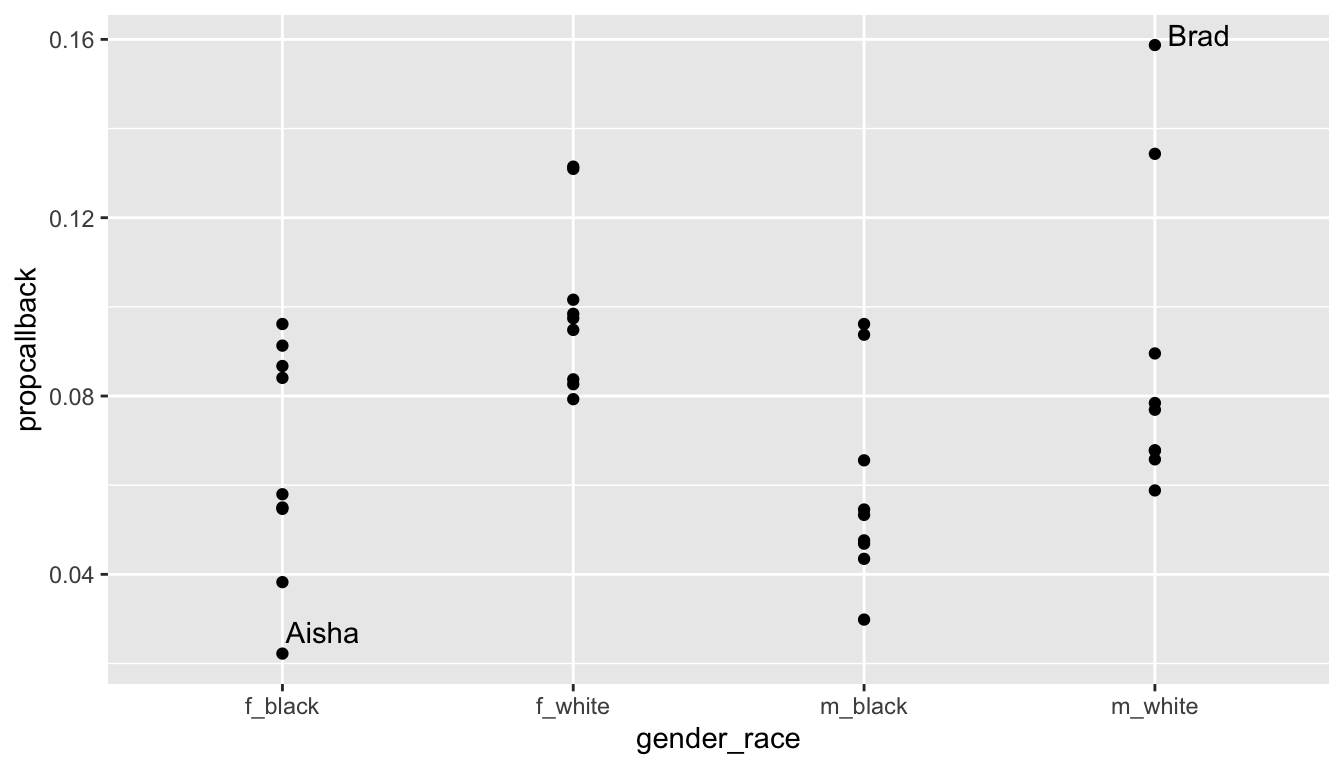
\includegraphics{01-intro_files/figure-latex/unnamed-chunk-10-1.pdf}

The x-axis corresponds to beer servings while the y-axis corresponds to wine servings. A reference line is given so with countries above the line consuming more wine than beer. We will get into how to make a plot like this later: for now, copy the code chunk and change the labeled point so that it corresponds to a country that interests you (other than Denmark).
We might be able to better answer the original question numerically by computing the wine to beer ratio for each country and then ordering from the largest ratio to the smallest ratio:

\begin{Shaded}
\begin{Highlighting}[]
\NormalTok{alcohol\_data }\SpecialCharTok{\%\textgreater{}\%}
  \FunctionTok{mutate}\NormalTok{(}\AttributeTok{wbratio =}\NormalTok{ wine\_servings }\SpecialCharTok{/}\NormalTok{ beer\_servings) }\SpecialCharTok{\%\textgreater{}\%}
  \FunctionTok{arrange}\NormalTok{(}\FunctionTok{desc}\NormalTok{(wbratio)) }\SpecialCharTok{\%\textgreater{}\%}
  \FunctionTok{select}\NormalTok{(country, beer\_servings, wine\_servings, wbratio)}
\CommentTok{\#\textgreater{} \# A tibble: 193 x 4}
\CommentTok{\#\textgreater{}    country             beer\_servings wine\_servings wbratio}
\CommentTok{\#\textgreater{}    \textless{}chr\textgreater{}                       \textless{}dbl\textgreater{}         \textless{}dbl\textgreater{}   \textless{}dbl\textgreater{}}
\CommentTok{\#\textgreater{}  1 Cook Islands                    0            74  Inf   }
\CommentTok{\#\textgreater{}  2 Qatar                           1             7    7   }
\CommentTok{\#\textgreater{}  3 Montenegro                     31           128    4.13}
\CommentTok{\#\textgreater{}  4 Timor{-}Leste                     1             4    4   }
\CommentTok{\#\textgreater{}  5 Syria                           5            16    3.2 }
\CommentTok{\#\textgreater{}  6 France                        127           370    2.91}
\CommentTok{\#\textgreater{}  7 Georgia                        52           149    2.87}
\CommentTok{\#\textgreater{}  8 Italy                          85           237    2.79}
\CommentTok{\#\textgreater{}  9 Equatorial Guinea              92           233    2.53}
\CommentTok{\#\textgreater{} 10 Sao Tome \& Principe            56           140    2.5 }
\CommentTok{\#\textgreater{} \# ... with 183 more rows}
\end{Highlighting}
\end{Shaded}

Why is one of the ratios \texttt{Inf}?

\hypertarget{exercise-1-1}{%
\subsection{Exercises}\label{exercise-1-1}}

\begin{enumerate}
\def\labelenumi{\arabic{enumi}.}
\item
  What is the shape of the distribution of total alcohol consumption? Left-skewed, right-skewed, or approximately symmetric? Unimodal or multimodal?
\item
  In the histogram of total alcohol consumption, pick a country other than the USA that interests you. See if you can change the code in the chunk that made the histogram so that the red vertical line is drawn for the country that interests you.
\end{enumerate}

Hint: Use the \texttt{View()} function to look at the alcohol data set by typing \texttt{View(alcohol\_data)} in your bottom-left window to help you see which countries are in the data set.

\begin{Shaded}
\begin{Highlighting}[]
\FunctionTok{View}\NormalTok{(alcohol\_data)}
\end{Highlighting}
\end{Shaded}

Note: careful about capitalization: \texttt{R} is case sensitive so USA is different than usa.

\begin{enumerate}
\def\labelenumi{\arabic{enumi}.}
\setcounter{enumi}{2}
\item
  In the histogram of total alcohol consumption, change the \textbf{fill} colour of the bins in the histogram above: what should be changed in the code chunk?
\item
  In the rankings code, what if you wanted to look at the top 5 countries instead of the top 3? See if you could change the code.
\item
  In the spirit rankings, why do you think only 2 countries showed up instead of 3? Can you do any investigation as to why this is the case?
\item
  Change the wine to beer ratio code example to find the countries with the highest beer to wine consumption (instead of wine to beer consumption).
\end{enumerate}

\hypertarget{athlete-data-example}{%
\section{Athlete Data Example}\label{athlete-data-example}}

Secondly, we will look at a data set on the top 100 highest paid athletes in 2014. The \texttt{athletesdata} was obtained from https://github.com/ali-ce/datasets data set has information on the following variables from the 100 highest paid athletes of 2014, according to Forbes (pay includes \textbf{both} salary and endorsements):

\begin{itemize}
\tightlist
\item
  \texttt{Name} (name of the athlete)
\item
  \texttt{Rank} (where the athlete ranks, with 1 being the highest paid)
\item
  \texttt{Sport} (the sport the athlete plays)
\item
  \texttt{endorsements} (money from sponsorships from companies)
\item
  \texttt{totalpay} (in millions in the year of 2014, salary + endorsements)
\item
  \texttt{salary} (money from tournaments or contract salary)
\item
  \texttt{age} of athlete in 2014
\item
  \texttt{Gender} (Male or Female)
\end{itemize}

We will first read in the data set below and name it \texttt{athletes}. We can then use the \texttt{head()} function to look at the first few rows of the data set.

\begin{Shaded}
\begin{Highlighting}[]
\NormalTok{athletes }\OtherTok{\textless{}{-}} \FunctionTok{read\_csv}\NormalTok{(}\StringTok{"data/athletesdata.csv"}\NormalTok{)}
\FunctionTok{head}\NormalTok{(athletes)}
\CommentTok{\#\textgreater{} \# A tibble: 6 x 9}
\CommentTok{\#\textgreater{}      X1 Name   Rank Sport endorsements totalpay salary   age}
\CommentTok{\#\textgreater{}   \textless{}dbl\textgreater{} \textless{}chr\textgreater{} \textless{}dbl\textgreater{} \textless{}chr\textgreater{}        \textless{}dbl\textgreater{}    \textless{}dbl\textgreater{}  \textless{}dbl\textgreater{} \textless{}dbl\textgreater{}}
\CommentTok{\#\textgreater{} 1     1 Aaro\textasciitilde{}    55 Foot\textasciitilde{}      7500000 22000000 1.45e7    31}
\CommentTok{\#\textgreater{} 2     2 Adam\textasciitilde{}    95 Golf       9000000 17700000 8.7 e6    34}
\CommentTok{\#\textgreater{} 3     3 Adri\textasciitilde{}    60 Base\textasciitilde{}       400000 21500000 2.11e7    32}
\CommentTok{\#\textgreater{} 4     4 Alex\textasciitilde{}    48 Base\textasciitilde{}       300000 22900000 2.26e7    39}
\CommentTok{\#\textgreater{} 5     5 Alfo\textasciitilde{}    93 Base\textasciitilde{}        50000 18050000 1.8 e7    38}
\CommentTok{\#\textgreater{} 6     6 Amar\textasciitilde{}    27 Bask\textasciitilde{}      5000000 26700000 2.17e7    32}
\CommentTok{\#\textgreater{} \# ... with 1 more variable: Gender \textless{}chr\textgreater{}}
\end{Highlighting}
\end{Shaded}

There are many different interesting questions to answer with this data set. First, we might be interested in the relationship between athlete age and salary for the top 100 athletes. Recall from an earlier stat course that one appropriate graphic to examine this relationship is a scatterplot:

\begin{Shaded}
\begin{Highlighting}[]
\FunctionTok{ggplot}\NormalTok{(}\AttributeTok{data =}\NormalTok{ athletes, }\AttributeTok{mapping =} \FunctionTok{aes}\NormalTok{(}\AttributeTok{x =}\NormalTok{ age, }\AttributeTok{y =}\NormalTok{ salary)) }\SpecialCharTok{+} 
  \FunctionTok{geom\_point}\NormalTok{() }\SpecialCharTok{+}
  \FunctionTok{geom\_smooth}\NormalTok{(}\AttributeTok{se =} \ConstantTok{FALSE}\NormalTok{)}
\end{Highlighting}
\end{Shaded}

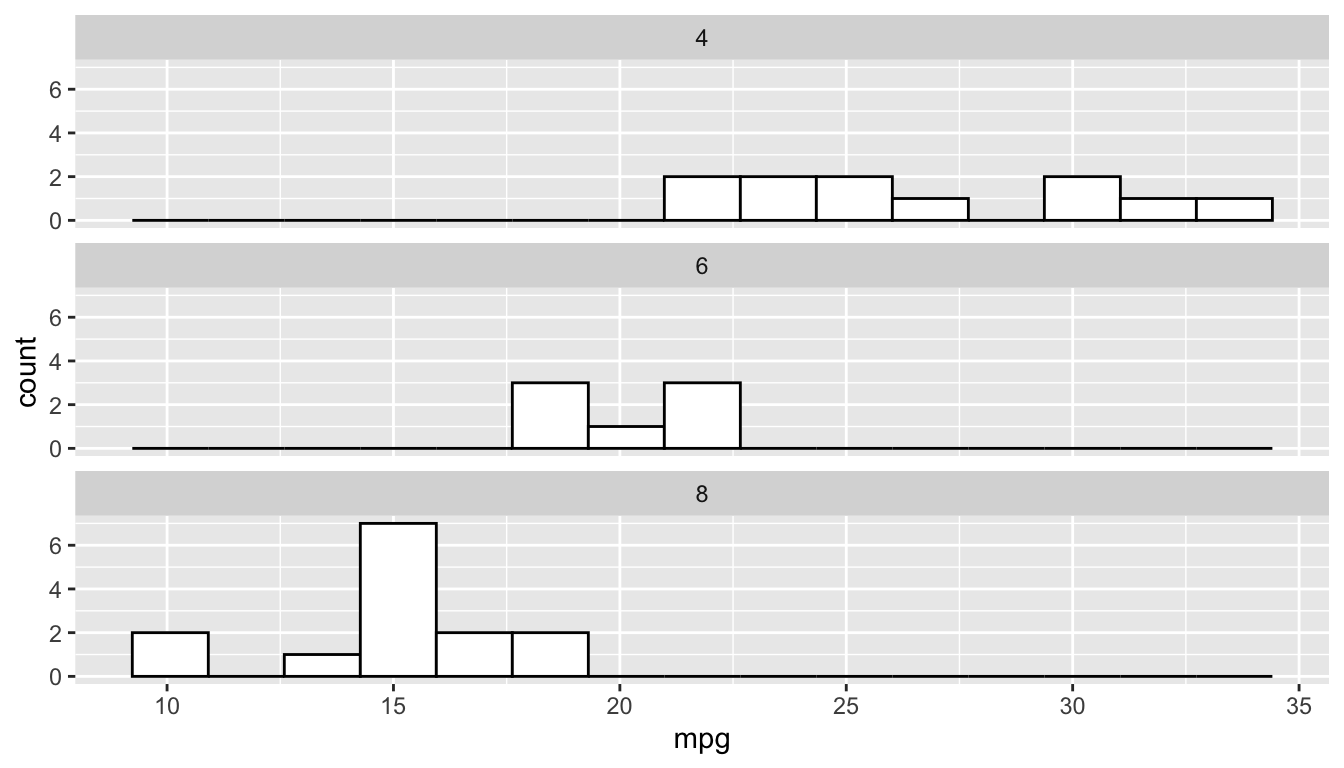
\includegraphics{01-intro_files/figure-latex/unnamed-chunk-14-1.pdf}

Do you see anything strange with the scatterplot? What do you think the y-axis tick labels of 2.5e+07, 5.0e+07, etc. mean?

Now let's see if we can count the number of athletes in the Top 100 that are in my personal favourite sport, Tennis:

\begin{Shaded}
\begin{Highlighting}[]
\NormalTok{athletes }\SpecialCharTok{\%\textgreater{}\%} \FunctionTok{group\_by}\NormalTok{(Sport) }\SpecialCharTok{\%\textgreater{}\%}
  \FunctionTok{summarise}\NormalTok{(}\AttributeTok{counts =} \FunctionTok{n}\NormalTok{()) }\SpecialCharTok{\%\textgreater{}\%}
  \FunctionTok{filter}\NormalTok{(Sport }\SpecialCharTok{==} \StringTok{"Tennis"}\NormalTok{)}
\CommentTok{\#\textgreater{} \# A tibble: 1 x 2}
\CommentTok{\#\textgreater{}   Sport  counts}
\CommentTok{\#\textgreater{}   \textless{}chr\textgreater{}   \textless{}int\textgreater{}}
\CommentTok{\#\textgreater{} 1 Tennis      6}
\end{Highlighting}
\end{Shaded}

It looks like there are 6 athletes: we can see who they are and sort them by their \texttt{Rank} with:

\begin{Shaded}
\begin{Highlighting}[]
\NormalTok{athletes }\SpecialCharTok{\%\textgreater{}\%}
  \FunctionTok{filter}\NormalTok{(Sport }\SpecialCharTok{==} \StringTok{"Tennis"}\NormalTok{) }\SpecialCharTok{\%\textgreater{}\%}
  \FunctionTok{arrange}\NormalTok{(Rank)}
\CommentTok{\#\textgreater{} \# A tibble: 6 x 9}
\CommentTok{\#\textgreater{}      X1 Name   Rank Sport endorsements totalpay salary   age}
\CommentTok{\#\textgreater{}   \textless{}dbl\textgreater{} \textless{}chr\textgreater{} \textless{}dbl\textgreater{} \textless{}chr\textgreater{}        \textless{}dbl\textgreater{}    \textless{}dbl\textgreater{}  \textless{}dbl\textgreater{} \textless{}dbl\textgreater{}}
\CommentTok{\#\textgreater{} 1    82 Roge\textasciitilde{}     7 Tenn\textasciitilde{}     52000000 56200000 4.2 e6    33}
\CommentTok{\#\textgreater{} 2    78 Rafa\textasciitilde{}     9 Tenn\textasciitilde{}     30000000 44500000 1.45e7    28}
\CommentTok{\#\textgreater{} 3    72 Nova\textasciitilde{}    17 Tenn\textasciitilde{}     21000000 33100000 1.21e7    27}
\CommentTok{\#\textgreater{} 4    64 Mari\textasciitilde{}    34 Tenn\textasciitilde{}     22000000 24400000 2.4 e6    27}
\CommentTok{\#\textgreater{} 5    60 Li Na    41 Tenn\textasciitilde{}     18000000 23600000 5.6 e6    32}
\CommentTok{\#\textgreater{} 6    89 Sere\textasciitilde{}    55 Tenn\textasciitilde{}     11000000 22000000 1.1 e7    33}
\CommentTok{\#\textgreater{} \# ... with 1 more variable: Gender \textless{}chr\textgreater{}}
\end{Highlighting}
\end{Shaded}

Finally, let's see if we can compare the ratio of endorsements (from commercials and products) to salary of professional athletes in the Top 100 in 2 sports: Football (referring to American Football) and Basketball. Recall from an earlier Stat class that we might want to use side-by-side boxplots to make this comparison since we have one categorical variable (Sport Type) and one quantitative variable (Ratio of Endorsements to Salary).

\begin{Shaded}
\begin{Highlighting}[]
\NormalTok{athletes }\SpecialCharTok{\%\textgreater{}\%} \FunctionTok{filter}\NormalTok{(Sport }\SpecialCharTok{==} \StringTok{"Football"} \SpecialCharTok{|}\NormalTok{ Sport }\SpecialCharTok{==} \StringTok{"Basketball"}\NormalTok{) }\SpecialCharTok{\%\textgreater{}\%}
  \FunctionTok{ggplot}\NormalTok{(}\AttributeTok{data =}\NormalTok{ ., }\FunctionTok{aes}\NormalTok{(}\AttributeTok{x =}\NormalTok{ Sport, }\AttributeTok{y =}\NormalTok{ endorsements }\SpecialCharTok{/}\NormalTok{ salary)) }\SpecialCharTok{+} 
  \FunctionTok{geom\_boxplot}\NormalTok{() }\SpecialCharTok{+}
  \FunctionTok{labs}\NormalTok{(}\AttributeTok{y =} \StringTok{"Endorsements / Salary"}\NormalTok{)}
\end{Highlighting}
\end{Shaded}

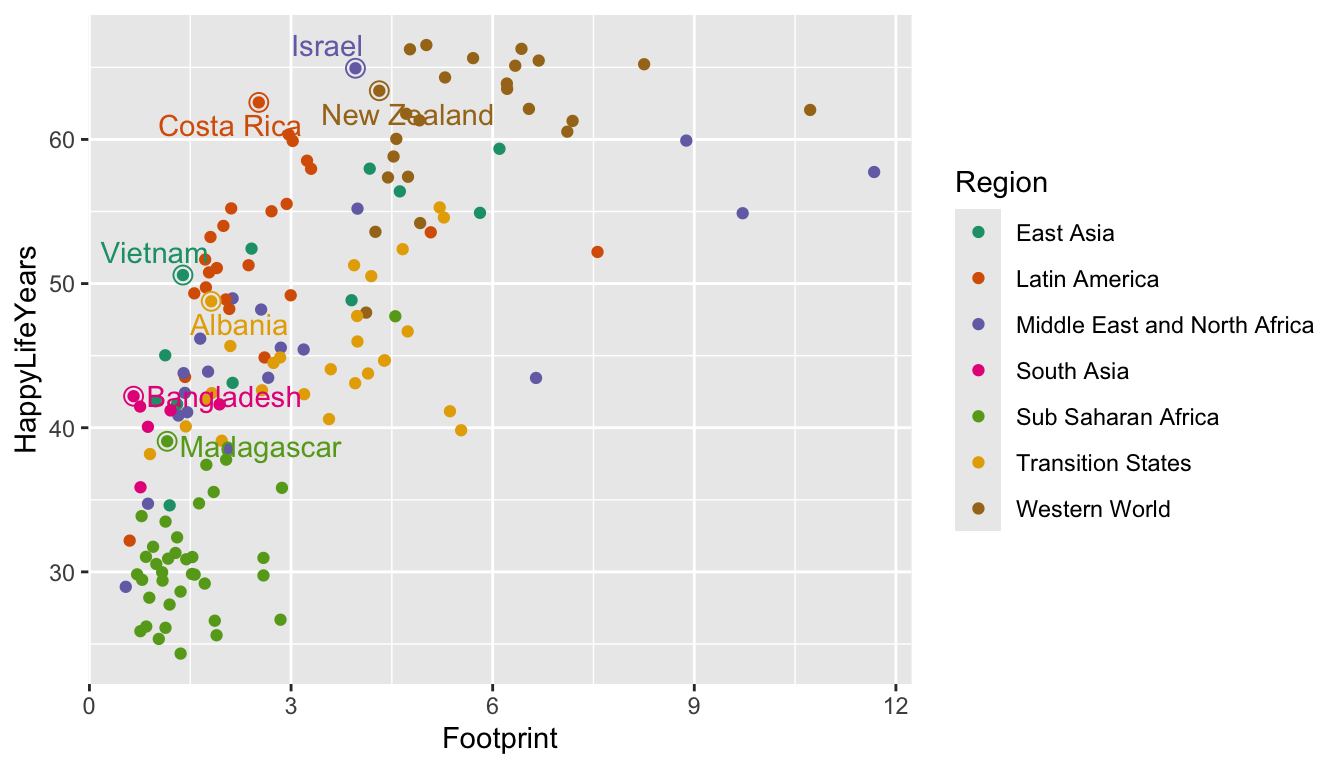
\includegraphics{01-intro_files/figure-latex/unnamed-chunk-17-1.pdf}

In the graph an endorsements / salary ratio of 1 indicates that the person makes half of their overall pay from endorsements and half of their overall pay from salary.

Which sport looks like it tends to receive a larger proportion of their overall pay from endorsements for athletes in the top 100?

\hypertarget{exercise-1-2}{%
\subsection{Exercises}\label{exercise-1-2}}

\begin{enumerate}
\def\labelenumi{\arabic{enumi}.}
\item
  Instead of looking at the relationship between age and salary in the top 100 athletes of 2014, change the plot to look at the relationship between age and endorsements. What would you change in the code above? Try it!
\item
  Pick a \texttt{Sport} other than Tennis and see if you can count the number of athletes in the top 100 in that sport as well as sort them by Rank. \textbf{Careful}: not all sports will have athletes in the Top 100.
\end{enumerate}

How many athletes are in the top 100 in the sport that you chose?

\begin{enumerate}
\def\labelenumi{\arabic{enumi}.}
\setcounter{enumi}{2}
\item
  In the endorsements / salary example, change one of the sports to the sport of your choice and make a comparison. Which sport tends to receive a larger proportion of their overall pay from endorsements.
\item
  What qualification might you want to make about your statement in the previous exercise? (Is this a random sample of athletes from each sport? Why does that matter?).
\item
  In the side-by-side boxplots comparing the endorsements to salary ratio of two different sports, I've changed the y-axis label above to be Endorsements / Salary using the \texttt{labs(y\ =\ "Endorsements\ /\ Salary")} statement. Try changing the x-axis label to something else. What do you think you would need to add to the plot?
\end{enumerate}

\hypertarget{finishing-up-common-errors-in-r}{%
\section{\texorpdfstring{Finishing Up: Common Errors in \texttt{R}}{Finishing Up: Common Errors in R}}\label{finishing-up-common-errors-in-r}}

We will now talk a little bit about getting errors in \texttt{R} and what can be done to correct some common errors.

You may have encountered some errors by this point in the document. Let's go over a few common errors as well as discuss how to comment your code.

\begin{enumerate}
\def\labelenumi{\arabic{enumi}.}
\tightlist
\item
  A missing parenthesis: any open parenthesis \texttt{(} \textbf{needs} to close \texttt{)}. Try running the following code chunk without fixing anything.
\end{enumerate}

\begin{Shaded}
\begin{Highlighting}[]
\FunctionTok{ggplot}\NormalTok{(}\AttributeTok{data =}\NormalTok{ athletes, }\FunctionTok{aes}\NormalTok{(}\AttributeTok{x =}\NormalTok{ Sport, }\AttributeTok{y =}\NormalTok{ salary) }\SpecialCharTok{+} 
  \FunctionTok{geom\_boxplot}\NormalTok{()}
\end{Highlighting}
\end{Shaded}

Notice in your bottom-left window that the \texttt{\textgreater{}} symbol that starts a line changes to a \texttt{+}. This is generally bad!! It means that you forgot to close a parenthesis \texttt{)} or a quote (\texttt{\textquotesingle{}} or \texttt{"}). No code will run since \texttt{R} thinks you are still trying to type something into a function. To fix this issue, click your cursor into the bottom-left window and press Esc. Then, try to find the error in the code chunk.

\begin{itemize}
\tightlist
\item
  Can you find the missing closing parenthesis above?
\end{itemize}

\begin{enumerate}
\def\labelenumi{\arabic{enumi}.}
\setcounter{enumi}{1}
\tightlist
\item
  Missing Comma. Try running the following code chunk without fixing anything.
\end{enumerate}

\begin{Shaded}
\begin{Highlighting}[]
\FunctionTok{ggplot}\NormalTok{(}\AttributeTok{data =}\NormalTok{ athletes }\FunctionTok{aes}\NormalTok{(}\AttributeTok{x =}\NormalTok{ Sport, }\AttributeTok{y =}\NormalTok{ salary)) }\SpecialCharTok{+} 
  \FunctionTok{geom\_boxplot}\NormalTok{()}
\end{Highlighting}
\end{Shaded}

\texttt{R} gives you an ``Error: unexpected symbol in \ldots.''. Oftentimes, this means that there is a missing comma or that you spelled a variable name incorrectly.

\begin{itemize}
\tightlist
\item
  Can you find the missed comma above?
\end{itemize}

\begin{enumerate}
\def\labelenumi{\arabic{enumi}.}
\setcounter{enumi}{2}
\tightlist
\item
  Capitalization Issues
\end{enumerate}

\begin{Shaded}
\begin{Highlighting}[]
\NormalTok{athletes }\SpecialCharTok{\%\textgreater{}\%} \FunctionTok{filter}\NormalTok{(sport }\SpecialCharTok{==} \StringTok{"Tennis"}\NormalTok{)}
\end{Highlighting}
\end{Shaded}

In the original data set, the variable \texttt{Sport} is capitalized. Not capitalizing it means that \texttt{R} won't be able to find it and proclaims that ``object sport not found''.

\begin{enumerate}
\def\labelenumi{\arabic{enumi}.}
\setcounter{enumi}{3}
\tightlist
\item
  Forgetting Quotes. Character strings need to have quotation marks around them. We will discuss more of this later, but graph labels and titles need to have quotes around them since they don't directly refer to columns or rows in our data set:
\end{enumerate}

\begin{Shaded}
\begin{Highlighting}[]
\FunctionTok{ggplot}\NormalTok{(}\AttributeTok{data =}\NormalTok{ athletes, }\FunctionTok{aes}\NormalTok{(}\AttributeTok{x =}\NormalTok{ Sport, }\AttributeTok{y =}\NormalTok{ endorsements)) }\SpecialCharTok{+} 
  \FunctionTok{geom\_boxplot}\NormalTok{() }\SpecialCharTok{+} \FunctionTok{xlab}\NormalTok{(Popularity Measure)}
\end{Highlighting}
\end{Shaded}

The error for forgetting quotes is typically an ``Unexpected Symbol'' though this error is also given for other issues.

\begin{itemize}
\tightlist
\item
  Where are the quotes missing in the code chunk above?
\end{itemize}

Finally, you can add a comment to a code chunk with the \texttt{\#} symbol (I always use double \texttt{\#\#} for some reason though). This allows you to type a comment into a code chunk that \textbf{isn't} code:

\begin{Shaded}
\begin{Highlighting}[]
\DocumentationTok{\#\# this is a comment}
\DocumentationTok{\#\# this calculation might be useful later}
\DecValTok{7} \SpecialCharTok{*} \DecValTok{42}
\CommentTok{\#\textgreater{} [1] 294}
\end{Highlighting}
\end{Shaded}

Comments are most useful for longer code chunks, as they allow you to remember why you did something. They also tell someone whom you've shared your code with why you did something.

Save this file by clicking File -\textgreater{} Save or by using the keyboard shortcut Command + s (or Control + s on a PC). Knit this file by clicking the Knit button in the top-left window (with the knitting needles). You should see a .html file pop up, if there are no errors in your code!

\hypertarget{chapexercise-1}{%
\section{Chapter Exercises}\label{chapexercise-1}}

\textbf{Note}: Usually, exercises will ask you to write code on your own using the week's chapter as a reference. However, for this initial chapter, we will do something a little different.

Open a new .Rmd file (File -\textgreater{} New File -\textgreater{} \texttt{R\ Markdown} -\textgreater{} OK) and delete the text explaining what \texttt{R\ Markdown} is in lines 10 and below. Then, complete the following exercises.

Exercise 1. Read the very short paper at https://joss.theoj.org/papers/10.21105/joss.01686 on an Introduction to the \texttt{tidyverse}, and answer the questions below in your \texttt{R\ Markdown} file. I'm imagining this whole exercise should only take you \textasciitilde{} 20-25 minutes.

Answer the following questions by typing answers in your .Rmd document. You should not need to make any new code chunks, as the questions don't ask you to do any coding!

\begin{enumerate}
\def\labelenumi{\arabic{enumi}.}
\item
  What are the two major areas that the \texttt{tidyverse} \textbf{doesn't} provide tools for?
\item
  How do the authors define ``tidy''?
\item
  What does it mean for the \texttt{tidyverse} to be ``human-centred''?
\item
  In about 2 sentences, describe the data science ``cycle'' given in the diagram at the top of page 3.
\end{enumerate}

Exercise 2. You may continue to use the same .Rmd file to answer these questions. For each question, type your answer on a new line, with a line space between your answers. All of these questions should be answered outside of code chunks since your answers will all be text, not code.

\begin{enumerate}
\def\labelenumi{\alph{enumi}.}
\item
  What is your name and what is your class year (first-year, sophomore, junior, senior)?
\item
  What is/are your major(s) and minor(s), either actual or intended?
\item
  Why are you taking this course? (Major requirement?, Minor requirement?, recommended by advisor or student?, exploring the field?, etc.).
\item
  In what semester and year did you take STAT 113 and who was your professor?
\item
  Have you taken STAT 213? Have you taken CS 140?
\item
  What is your hometown: city, state, country?
\item
  Do you play a sport on campus? If so, what sport? If not, what is an activity that you do on or off-campus?
\item
  What is your favorite TV show or movie or band/musical artist?
\item
  Tell me something about yourself.
\item
  Take a look at the learning outcomes listed on the syllabus. Which are you most excited for and why?
\item
  What are your expectations for this class and/or what do you hope to gain from this class?
\end{enumerate}

Knit your .Rmd file into an .html file and submit your knitted .html file to Sakai. If your file won't knit, then submit the .Rmd file instead. To submit either file, you first need to get the file off of the server and onto your computer so that you can upload it to Sakai. Use the following steps to do so:

\begin{enumerate}
\def\labelenumi{\arabic{enumi}.}
\item
  Click the checkbox next to your knitted .html file.
\item
  Click the Gear Icon ``More'' -\textgreater{} Export
\item
  If you would like, rename your file to something like Week0\_YOURLASTNAME.html, but, make sure to keep the correct extension (either .html or .Rmd).
\item
  After you export it, the file should appear in your downloads folder. Now, go to Sakai -\textgreater{} Assignments -\textgreater{} Week 0 Exercises and complete the upload process.
\end{enumerate}

Nice work: we will dive into \texttt{ggplot()} in the \texttt{ggplot2} package next!

\hypertarget{solutions-1}{%
\section{Exercise Solutions}\label{solutions-1}}

In most sections, some exercise solutions will be posted at the end of the section. However, for the introduction, we will do all of the coding exercises as a class to make sure that we all start off well.

\hypertarget{ggplot2}{%
\chapter{\texorpdfstring{Plotting with \texttt{ggplot2}}{Plotting with ggplot2}}\label{ggplot2}}

\textbf{Goals:}

\begin{enumerate}
\def\labelenumi{\arabic{enumi}.}
\item
  Use the \texttt{ggplot2} package to make exploratory plots from STAT 113 of a single quantitative variable, two quantitative variables, a quantitative and a categorical variable, a single categorical variable, and two categorical variables.
\item
  Use the plots produced to answer questions about the Presidential election data set and the Fitness data set.
\item
  Further practice running code in \texttt{R}.
\end{enumerate}

\hypertarget{introduction-and-basic-terminology}{%
\section{Introduction and Basic Terminology}\label{introduction-and-basic-terminology}}

We will begin our data science journey with plotting in the \texttt{ggplot2} package. We are starting with plotting for a couple of reasons:

\begin{enumerate}
\def\labelenumi{\arabic{enumi}.}
\item
  Plotting is cool! We get to see an immediate result of our coding efforts in the form of a nice-to-look-at plot.
\item
  In an exploratory data analysis, you would typically start by making plots of your data.
\item
  Plotting can lead us to ask and subsequently investigate interesting questions, as we will see in our first example.
\end{enumerate}

We will first use a data set on the 2000 United States Presidential election between former President George Bush and Al Gore obtained from http://www.econometrics.com/intro/votes.htm. For those unfamiliar with U.S. political elections, it is enough to know that each state is allocated a certain number of ``electoral votes'' for the president: states award all of their electoral votes to the candidate that receives the most ballots in that state. You can read more about this strange system on Wikipedia.

Florida is typically a highly-contentious ``battleground'' state. The data set that we have has the following variables, recorded for each of the 67 counties in Florida:

\begin{itemize}
\tightlist
\item
  \texttt{Gore}, the number of people who voted for Al Gore in 2000
\item
  \texttt{Bush}, the number of people who voted for George Bush in 2000
\item
  \texttt{Buchanan}, the number of people who voted for the third-party candidate Buchanan
\item
  \texttt{Nader}, the number of people who voted for the third-party candidate Nader
\item
  \texttt{Other}, the number of people who voted for a candidate other than the previous 4 listed
\item
  \texttt{County}, the name of the county in Florida
\end{itemize}

To get started exploring the data, complete the following steps that you learned in Week 0:

\begin{enumerate}
\def\labelenumi{\arabic{enumi}.}
\item
  Log-on to the SLU \texttt{R\ Studio} server http://rstudio.stlawu.local:8787
\item
  Create a new .Rmd file in the same folder as your Notes \texttt{R\ Project} using File -\textgreater{} New File -\textgreater{} \texttt{R\ Markdown}.
\item
  Finally, read in and name the data set \texttt{pres\_df}, and take a look at the data set by running the \texttt{head(pres\_df)} line, which shows the first few observations of the data set:
\end{enumerate}

\begin{Shaded}
\begin{Highlighting}[]
\FunctionTok{library}\NormalTok{(tidyverse)}
\NormalTok{pres\_df }\OtherTok{\textless{}{-}} \FunctionTok{read\_table}\NormalTok{(}\StringTok{"data/PRES2000.txt"}\NormalTok{) }
\DocumentationTok{\#\# don\textquotesingle{}t worry about the \textasciigrave{}read\_table\textasciigrave{} function....yet}
\FunctionTok{head}\NormalTok{(pres\_df)}
\CommentTok{\#\textgreater{} \# A tibble: 6 x 6}
\CommentTok{\#\textgreater{}     Gore   Bush Buchanan Nader Other County  }
\CommentTok{\#\textgreater{}    \textless{}dbl\textgreater{}  \textless{}dbl\textgreater{}    \textless{}dbl\textgreater{} \textless{}dbl\textgreater{} \textless{}dbl\textgreater{} \textless{}chr\textgreater{}   }
\CommentTok{\#\textgreater{} 1  47365  34124      263  3226   751 ALACHUA }
\CommentTok{\#\textgreater{} 2   2392   5610       73    53    26 BAKER   }
\CommentTok{\#\textgreater{} 3  18850  38637      248   828   242 BAY     }
\CommentTok{\#\textgreater{} 4   3075   5414       65    84    35 BRADFORD}
\CommentTok{\#\textgreater{} 5  97318 115185      570  4470   852 BREVARD }
\CommentTok{\#\textgreater{} 6 386561 177323      788  7101  1623 BROWAR}
\end{Highlighting}
\end{Shaded}

Pay special attention to the variable names: we'll need to use these names when we make all of our plots. And, \texttt{R} is case-sensitive, meaning that we will, for example, need to use \texttt{Gore}, not \texttt{gore}.

We are trying to go very light on the technical code terminology to start out with (but we will come back to some things later in the semester). The terminology will make a lot more sense once you've actually worked with data. But, there are three terms that will be thrown around quite a bit in the next few weeks: \emph{function}, \emph{argument}, and \emph{object}.

\begin{itemize}
\item
  a \emph{function} in \texttt{R} is always* (*always for this class) followed by an open \texttt{(} and ended with a closed \texttt{)}. In non-technical terms, a \emph{function} \textbf{does} something to its inputs and is often analogous to an English verb. For example, the \texttt{mean()} function calculates the mean, the \texttt{rank()} functions ranks a variable from lowest to highest, and the \texttt{labs()} is used to add labels to a plot. Every function has a help file that can be accessed by typing in \texttt{?name\_of\_function}. Try typing \texttt{?mean} in your lower left window.
\item
  an \emph{argument} is something that goes inside the parentheses in a function. Arguments could include \emph{objects}, or they might not. In the bottom-left window, type \texttt{?mean} to view the Help file on this \texttt{R} function. We see that \texttt{mean()} has 3 arguments: \texttt{x}, which is an \texttt{R} object, \texttt{trim}, and \texttt{na.rm}. \texttt{trim\ =\ 0} is the default, which means that, by default, \texttt{R} will not trim any of the numbers when computing the mean.
\item
  an \emph{object} is something created in \texttt{R}, usually with \texttt{\textless{}-}. So, looking at the code above where we read in the data, \texttt{pres\_df} is an \texttt{R} object.
\end{itemize}

All of this will make more sense as we go through these first couple of weeks.

\hypertarget{basic-plot-structure}{%
\section{Basic Plot Structure}\label{basic-plot-structure}}

We will use the \texttt{ggplot()} function in the \texttt{ggplot2} package to construct visualizations of data. the \texttt{ggplot()} function has 3 basic components:

\begin{itemize}
\tightlist
\item
  a \texttt{data} argument, specifying the name of your data set (\texttt{pres\_df} above)
\item
  a \texttt{mapping} argument, specifying that specifies the aesthetics of your plot (\texttt{aes()}). Common aesthetics are \texttt{x} position, \texttt{y} position, \texttt{colour}, \texttt{size}, \texttt{shape}, \texttt{group}, and \texttt{fill}.
\item
  a \texttt{geom\_\ \ \ \ ()} component, specifying the geometric shape used to display the data.
\end{itemize}

The components are combined in the following form:

\begin{Shaded}
\begin{Highlighting}[]
\FunctionTok{ggplot}\NormalTok{(}\AttributeTok{data =}\NormalTok{ name\_of\_data, }\AttributeTok{mapping =} \FunctionTok{aes}\NormalTok{(}\AttributeTok{x =}\NormalTok{ name\_of\_x\_var, }
                                          \AttributeTok{y =}\NormalTok{ name\_of\_y\_var,}
                                          \AttributeTok{colour =}\NormalTok{ name\_of\_colour\_var,}
\NormalTok{                                          etc.)) }\SpecialCharTok{+}
  \FunctionTok{geom\_nameofgeom}\NormalTok{() }\SpecialCharTok{+}
\NormalTok{  .....}\SpecialCharTok{\textless{}}\NormalTok{other stuff}\SpecialCharTok{\textgreater{}}
\end{Highlighting}
\end{Shaded}

The structure of \texttt{ggplot()} plots is based on the Grammar of Graphics https://www.springer.com/gp/book/9780387245447. As with most new things, the components above will be easier to think about with some examples.

\hypertarget{graphing-a-single-variable}{%
\section{Graphing a Single Variable}\label{graphing-a-single-variable}}

\hypertarget{histograms-and-frequency-plots-for-a-quantitative-variable}{%
\subsection{Histograms and Frequency Plots for a Quantitative Variable}\label{histograms-and-frequency-plots-for-a-quantitative-variable}}

Let's go ahead and begin our exploration of the data by making a histogram of the number of people who voted for \texttt{Gore} in each county. Recall that a histogram is useful if we would like a graph of a single quantitative variable. Copy the following code to an \texttt{R} chunk and run the code:

\begin{Shaded}
\begin{Highlighting}[]
\FunctionTok{ggplot}\NormalTok{(}\AttributeTok{data =}\NormalTok{ pres\_df, }\AttributeTok{mapping =} \FunctionTok{aes}\NormalTok{(}\AttributeTok{x =}\NormalTok{ Gore)) }\SpecialCharTok{+}
  \FunctionTok{geom\_histogram}\NormalTok{(}\AttributeTok{colour =} \StringTok{"black"}\NormalTok{, }\AttributeTok{fill =} \StringTok{"white"}\NormalTok{) }\SpecialCharTok{+}
  \FunctionTok{xlab}\NormalTok{(}\StringTok{"Votes for Gore in Florida"}\NormalTok{)}
\CommentTok{\#\textgreater{} \textasciigrave{}stat\_bin()\textasciigrave{} using \textasciigrave{}bins = 30\textasciigrave{}. Pick better value with}
\CommentTok{\#\textgreater{} \textasciigrave{}binwidth\textasciigrave{}.}
\end{Highlighting}
\end{Shaded}

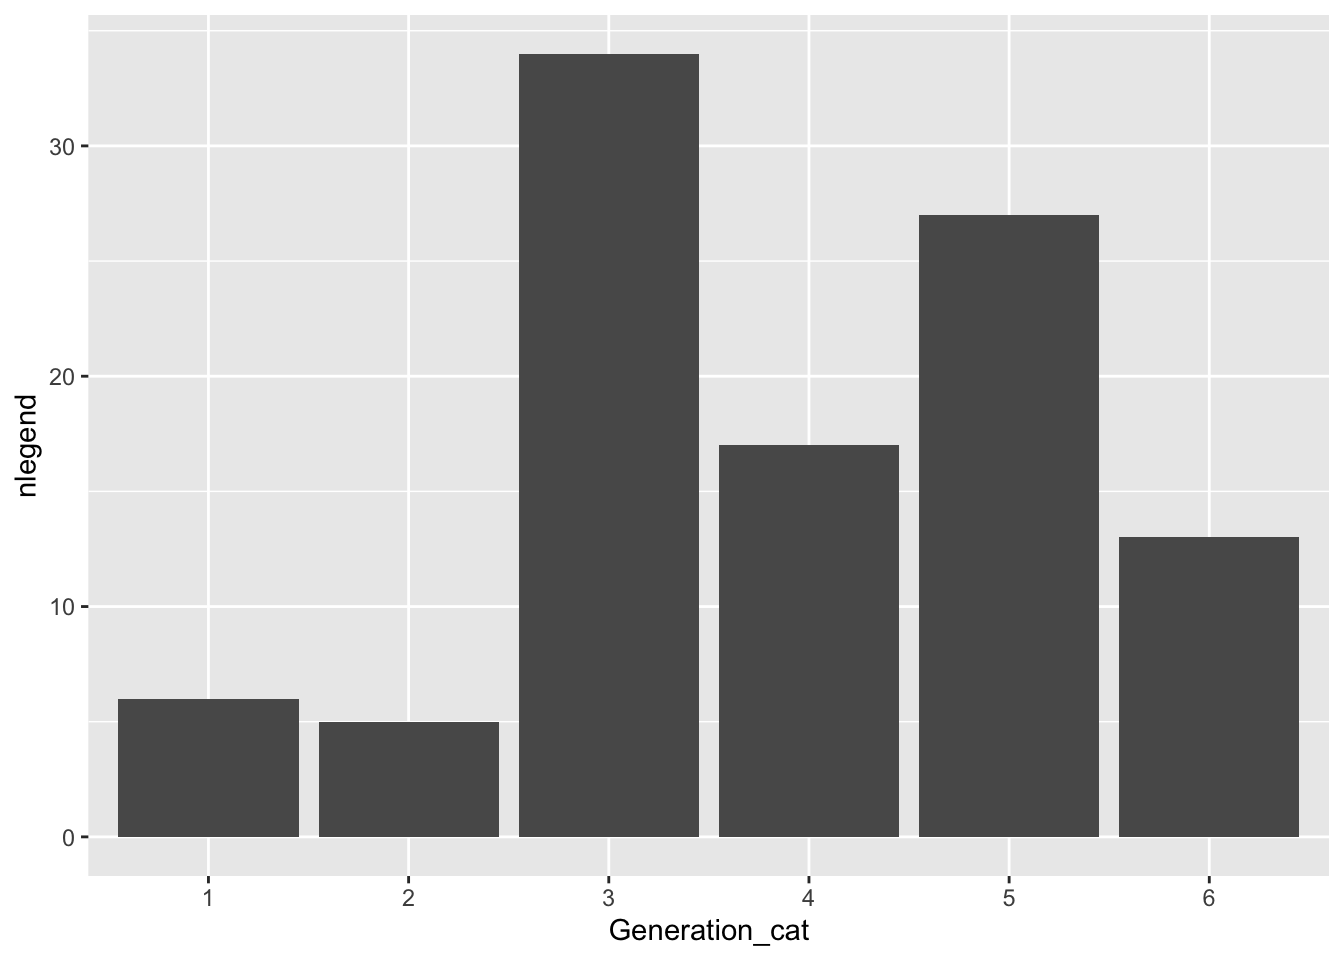
\includegraphics{02-ggplot2_files/figure-latex/unnamed-chunk-3-1.pdf}

What do the 1e+05, 2e+05, etc. labels on the x-axis mean?

\texttt{R} gives us a message to ``Pick a better value with \texttt{binwidth}'' instead of the default \texttt{bins\ =\ 30}. Add \texttt{,\ bins\ =\ 15} inside the parentheses of \texttt{geom\_histogram()} to change the number of bins in the histogram.

Change the colour of the inside of the bins to ``darkred''. Do you think that the colour of the inside of the bins maps to \texttt{colour} or \texttt{fill}? Try both!

There are a couple of observations with very high vote values. What could explain these large outliers?

Another graph useful in visualizing a single quantitative variable is a frequency plot. The code to make a frequency plot is given below. We are simply replacing \texttt{geom\_histogram()} with \texttt{geom\_freqpoly()}.

\begin{Shaded}
\begin{Highlighting}[]
\FunctionTok{ggplot}\NormalTok{(}\AttributeTok{data =}\NormalTok{ pres\_df, }\AttributeTok{mapping =} \FunctionTok{aes}\NormalTok{(}\AttributeTok{x =}\NormalTok{ Gore)) }\SpecialCharTok{+}
  \FunctionTok{geom\_freqpoly}\NormalTok{(}\AttributeTok{colour =} \StringTok{"black"}\NormalTok{) }\SpecialCharTok{+}
  \FunctionTok{xlab}\NormalTok{(}\StringTok{"Votes for Gore in Florida"}\NormalTok{) }
\CommentTok{\#\textgreater{} \textasciigrave{}stat\_bin()\textasciigrave{} using \textasciigrave{}bins = 30\textasciigrave{}. Pick better value with}
\CommentTok{\#\textgreater{} \textasciigrave{}binwidth\textasciigrave{}.}
\end{Highlighting}
\end{Shaded}

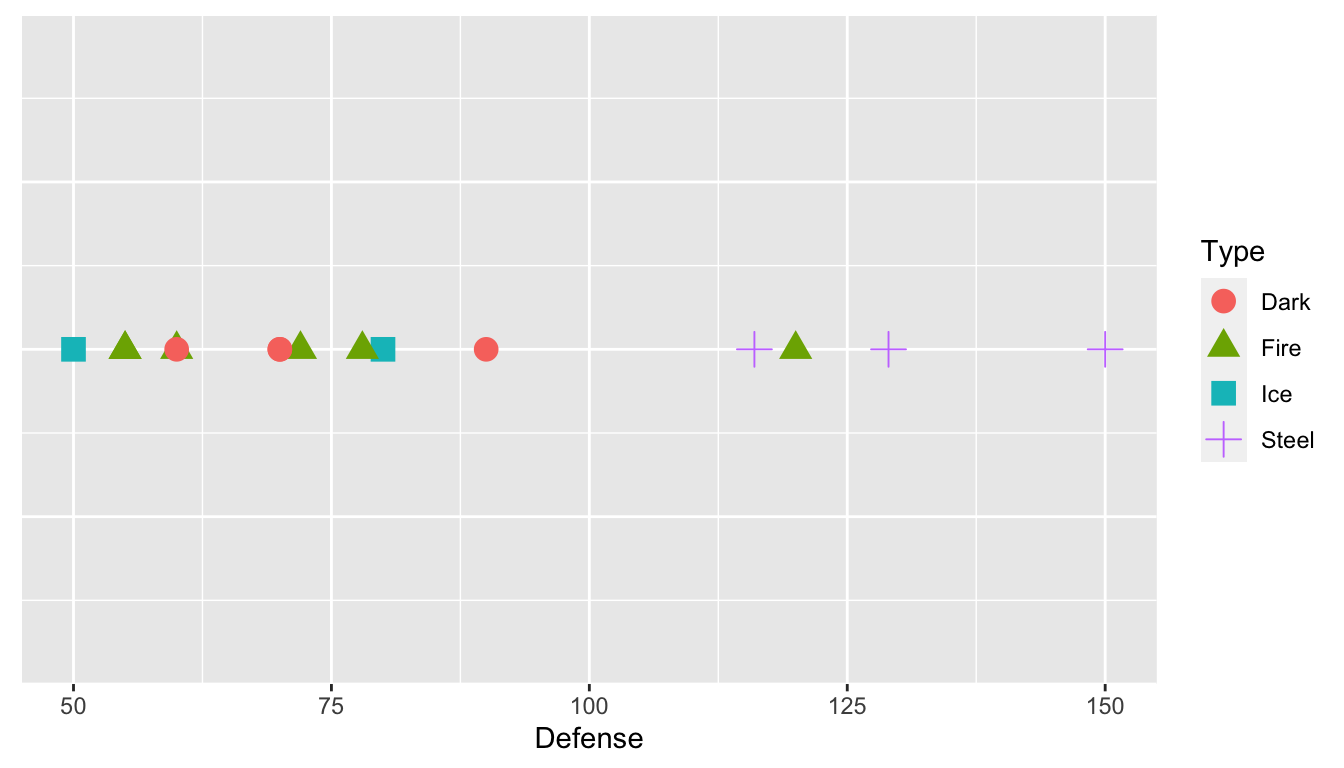
\includegraphics{02-ggplot2_files/figure-latex/unnamed-chunk-4-1.pdf}

The frequency plot is just like a histogram but the counts are connected by a line instead of represented with bins. You can see how they relate by including \textbf{both} a geom\_freqpoly() and a geom\_histogram() in your plot, though it doesn't make for the prettiest graph:

\begin{Shaded}
\begin{Highlighting}[]
\FunctionTok{ggplot}\NormalTok{(}\AttributeTok{data =}\NormalTok{ pres\_df, }\AttributeTok{mapping =} \FunctionTok{aes}\NormalTok{(}\AttributeTok{x =}\NormalTok{ Gore)) }\SpecialCharTok{+}
  \FunctionTok{geom\_freqpoly}\NormalTok{(}\AttributeTok{colour =} \StringTok{"black"}\NormalTok{) }\SpecialCharTok{+}
  \FunctionTok{xlab}\NormalTok{(}\StringTok{"Votes for Gore in Florida"}\NormalTok{) }\SpecialCharTok{+}
  \FunctionTok{geom\_histogram}\NormalTok{() }
\CommentTok{\#\textgreater{} \textasciigrave{}stat\_bin()\textasciigrave{} using \textasciigrave{}bins = 30\textasciigrave{}. Pick better value with}
\CommentTok{\#\textgreater{} \textasciigrave{}binwidth\textasciigrave{}.}
\CommentTok{\#\textgreater{} \textasciigrave{}stat\_bin()\textasciigrave{} using \textasciigrave{}bins = 30\textasciigrave{}. Pick better value with}
\CommentTok{\#\textgreater{} \textasciigrave{}binwidth\textasciigrave{}.}
\end{Highlighting}
\end{Shaded}

\includegraphics{02-ggplot2_files/figure-latex/unnamed-chunk-5-1.pdf}

\hypertarget{r-code-style}{%
\subsection{\texorpdfstring{\texttt{R} Code Style}{R Code Style}}\label{r-code-style}}

We want our code to be as readable as possible. This not only benefits other people who may read your code (like me), but it also benefits you, particularly if you read your own code in the future. I try to follow the Style Guide in the Advanced \texttt{R} book: http://adv-r.had.co.nz/Style.html. Feel free to skim through that, but you don't need to worry about it too much: you should be able to pick up on some important elements just from going through this course. You might actually end up having better code style if you \emph{haven't} had any previous coding experience.

As a quick example of why code style can be important, consider the following two code chunks, both of which produce the same graph.

\begin{Shaded}
\begin{Highlighting}[]
\FunctionTok{ggplot}\NormalTok{(}\AttributeTok{data=}\NormalTok{pres\_df,}\AttributeTok{mapping=}\FunctionTok{aes}\NormalTok{(}\AttributeTok{x=}\NormalTok{Gore))}\SpecialCharTok{+}\FunctionTok{geom\_histogram}\NormalTok{(}\AttributeTok{colour=}\StringTok{"black"}\NormalTok{,}\AttributeTok{fill=}\StringTok{"white"}\NormalTok{)}\SpecialCharTok{+}
  \FunctionTok{xlab}\NormalTok{(}\StringTok{"Votes for Gore in Florida"}\NormalTok{)}
\end{Highlighting}
\end{Shaded}

\begin{Shaded}
\begin{Highlighting}[]
\FunctionTok{ggplot}\NormalTok{(}\AttributeTok{data =}\NormalTok{ pres\_df, }\AttributeTok{mapping =} \FunctionTok{aes}\NormalTok{(}\AttributeTok{x =}\NormalTok{ Gore)) }\SpecialCharTok{+}
  \FunctionTok{geom\_histogram}\NormalTok{(}\AttributeTok{colour =} \StringTok{"black"}\NormalTok{, }\AttributeTok{fill =} \StringTok{"white"}\NormalTok{) }\SpecialCharTok{+}
  \FunctionTok{xlab}\NormalTok{(}\StringTok{"Votes for Gore in Florida"}\NormalTok{)}
\end{Highlighting}
\end{Shaded}

Which code chunk would you want to read two years from now? Which code chunk would you want your classmate/friend/coworker to read? (assuming you like your classmate/friend/coworker\ldots.)

\hypertarget{bar-plots-for-a-categorical-variable}{%
\subsection{Bar Plots for a Categorical Variable}\label{bar-plots-for-a-categorical-variable}}

Recall from STAT 113 that bar plots are useful if you want to examine the distribution of one categorical variable. Side-by-side bar plots or stacked bar plots are plots that are useful for looking at the relationship between two categorical variables. There actually aren't any categorical variables that would be interesting to plot in this data set, so we'll make one, called \texttt{winner} using code that we don't need to understand until next week. \texttt{winner} will be \texttt{"Gore"} if Gore won the county and \texttt{"Bush"} if Bush won the county. We'll name this new data set \texttt{pres\_cat}.

\begin{Shaded}
\begin{Highlighting}[]
\NormalTok{pres\_cat }\OtherTok{\textless{}{-}}\NormalTok{ pres\_df }\SpecialCharTok{\%\textgreater{}\%} \FunctionTok{mutate}\NormalTok{(}\AttributeTok{winner =} \FunctionTok{if\_else}\NormalTok{(Gore }\SpecialCharTok{\textgreater{}}\NormalTok{ Bush,}
                                                \AttributeTok{true =} \StringTok{"Gore"}\NormalTok{,}
                                                \AttributeTok{false =} \StringTok{"Bush"}\NormalTok{))}
\NormalTok{pres\_cat}
\CommentTok{\#\textgreater{} \# A tibble: 67 x 7}
\CommentTok{\#\textgreater{}      Gore   Bush Buchanan Nader Other County    winner}
\CommentTok{\#\textgreater{}     \textless{}dbl\textgreater{}  \textless{}dbl\textgreater{}    \textless{}dbl\textgreater{} \textless{}dbl\textgreater{} \textless{}dbl\textgreater{} \textless{}chr\textgreater{}     \textless{}chr\textgreater{} }
\CommentTok{\#\textgreater{}  1  47365  34124      263  3226   751 ALACHUA   Gore  }
\CommentTok{\#\textgreater{}  2   2392   5610       73    53    26 BAKER     Bush  }
\CommentTok{\#\textgreater{}  3  18850  38637      248   828   242 BAY       Bush  }
\CommentTok{\#\textgreater{}  4   3075   5414       65    84    35 BRADFORD  Bush  }
\CommentTok{\#\textgreater{}  5  97318 115185      570  4470   852 BREVARD   Bush  }
\CommentTok{\#\textgreater{}  6 386561 177323      788  7101  1623 BROWAR    Gore  }
\CommentTok{\#\textgreater{}  7   2155   2873       90    39    17 CALHOUN   Bush  }
\CommentTok{\#\textgreater{}  8  29645  35426      182  1462   181 CHARLOTTE Bush  }
\CommentTok{\#\textgreater{}  9  25525  29765      270  1379   261 CITRUS    Bush  }
\CommentTok{\#\textgreater{} 10  14632  41736      186   562   237 CLAY      Bush  }
\CommentTok{\#\textgreater{} \# ... with 57 more rows}
\end{Highlighting}
\end{Shaded}

Using this data set, we can make a bar plot with \texttt{geom\_bar()}. The beauty of \texttt{ggplot()} is that the code is super-similar to what we used for histograms and frequency plots!

\begin{Shaded}
\begin{Highlighting}[]
\FunctionTok{ggplot}\NormalTok{(}\AttributeTok{data =}\NormalTok{ pres\_cat, }\FunctionTok{aes}\NormalTok{(}\AttributeTok{x =}\NormalTok{ winner)) }\SpecialCharTok{+}
  \FunctionTok{geom\_bar}\NormalTok{()}
\end{Highlighting}
\end{Shaded}

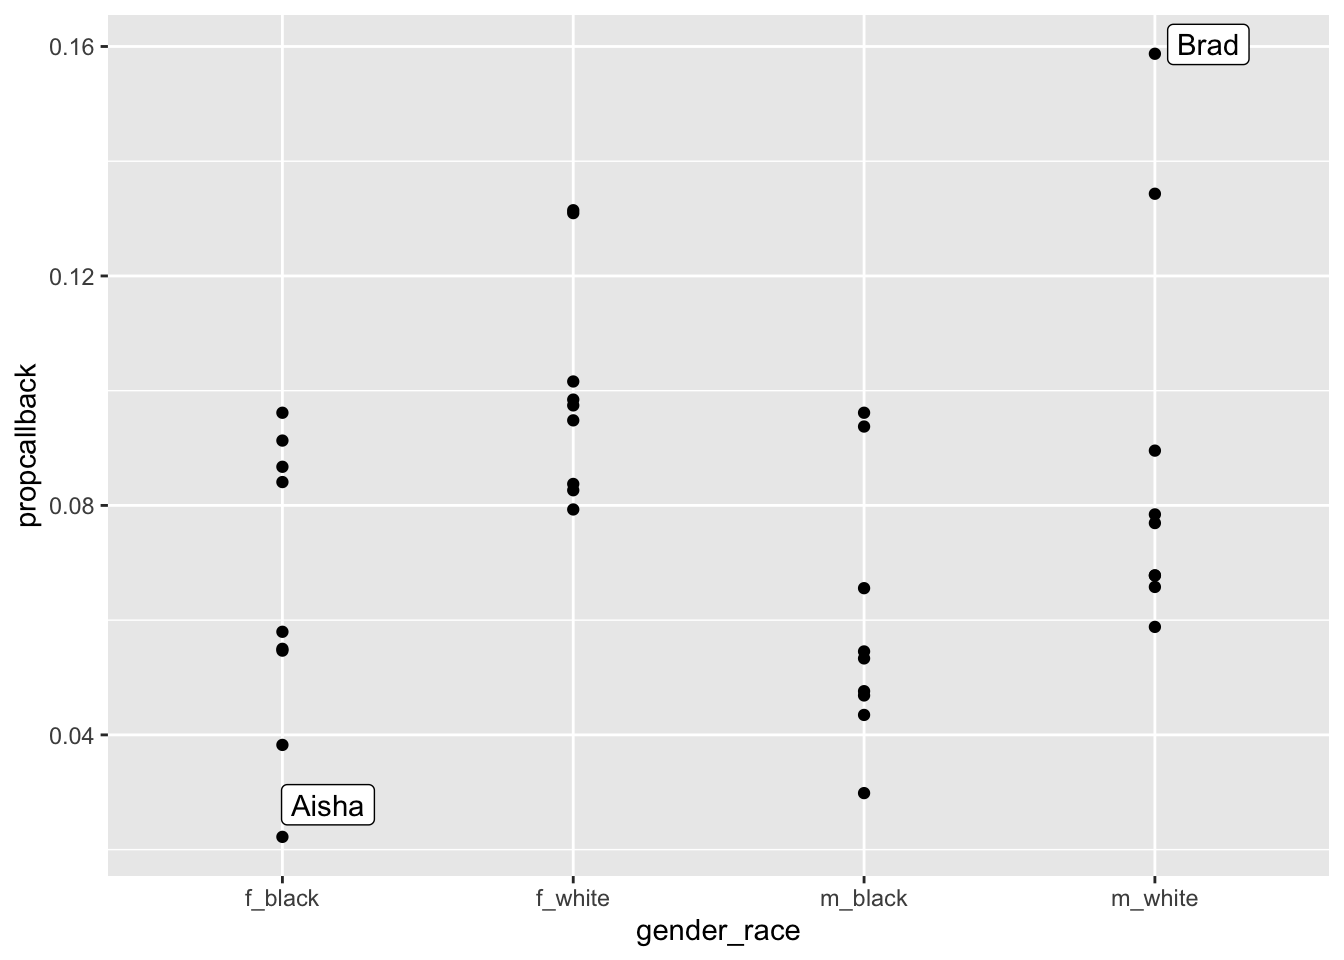
\includegraphics{02-ggplot2_files/figure-latex/unnamed-chunk-9-1.pdf}

Note that, sometimes, data are in format such that one column contains the \emph{levels} of the categorical variable while another column contains the counts directly. For example, we can create such a data set using code that we will learn next week:

\begin{Shaded}
\begin{Highlighting}[]
\NormalTok{pres\_cat2 }\OtherTok{\textless{}{-}}\NormalTok{ pres\_cat }\SpecialCharTok{\%\textgreater{}\%} \FunctionTok{group\_by}\NormalTok{(winner) }\SpecialCharTok{\%\textgreater{}\%}
  \FunctionTok{summarise}\NormalTok{(}\AttributeTok{nwins =} \FunctionTok{n}\NormalTok{())}
\NormalTok{pres\_cat2}
\CommentTok{\#\textgreater{} \# A tibble: 2 x 2}
\CommentTok{\#\textgreater{}   winner nwins}
\CommentTok{\#\textgreater{}   \textless{}chr\textgreater{}  \textless{}int\textgreater{}}
\CommentTok{\#\textgreater{} 1 Bush      51}
\CommentTok{\#\textgreater{} 2 Gore      16}
\end{Highlighting}
\end{Shaded}

This data set has just two observations and contains a column for the two major presidential candidates and a column for the number of counties that each candidate won. If we wanted to make a barplot showing the number of wins for each candidate, we can't use \texttt{geom\_bar()}. Predict what the result will be from running the following code.

\begin{Shaded}
\begin{Highlighting}[]
\FunctionTok{ggplot}\NormalTok{(pres\_cat2, }\FunctionTok{aes}\NormalTok{(}\AttributeTok{x =}\NormalTok{ winner)) }\SpecialCharTok{+}
  \FunctionTok{geom\_bar}\NormalTok{()}
\end{Highlighting}
\end{Shaded}

Instead, we can use \texttt{geom\_col()}, which takes an \texttt{x} aesthetic giving the column with names of the levels of our categorical variable, and a \texttt{y} aesthetic giving the column with the counts:

\begin{Shaded}
\begin{Highlighting}[]
\FunctionTok{ggplot}\NormalTok{(pres\_cat2, }\FunctionTok{aes}\NormalTok{(}\AttributeTok{x =}\NormalTok{ winner, }\AttributeTok{y =}\NormalTok{ nwins)) }\SpecialCharTok{+}
  \FunctionTok{geom\_col}\NormalTok{()}
\end{Highlighting}
\end{Shaded}

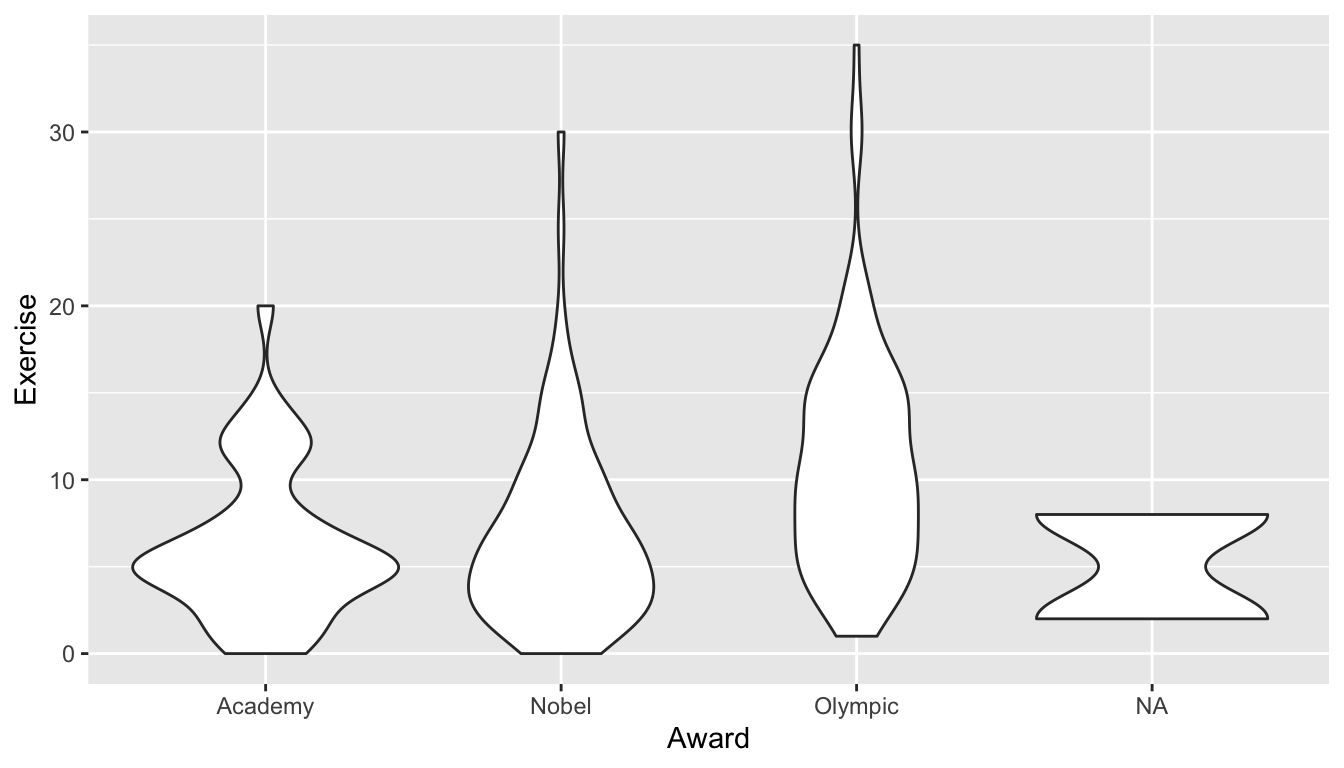
\includegraphics{02-ggplot2_files/figure-latex/unnamed-chunk-12-1.pdf}

\hypertarget{exercise-2-1}{%
\subsection{Exercises}\label{exercise-2-1}}

Exercises marked with an * indicate that the exercise has a solution at the end of the chapter at \ref{solutions-2}.

\begin{enumerate}
\def\labelenumi{\arabic{enumi}.}
\item
  Change the frequency plot to plot the number of votes for Bush instead of the number for Gore. Are there any obvious outliers in the Bush frequency plot?
\item
  Do you have a preference for histograms or a preference for frequency plots? Can you think of a situation where one would be more desirable than the other?
\item
  It looks like Bush won a lot more\ldots.does that necessarily mean that Bush won more votes in total in Florida? Why or why not?
\end{enumerate}

We will be using survey data from STAT 113 in the 2018-2019 academic year for many exercises in this section. For those who may not have taken STAT 113 from having AP credit or another reason, the STAT 113 survey is given to all students in STAT 113 across all sections. Some analyses in Intro Stat are then carried out using the survey.

\begin{Shaded}
\begin{Highlighting}[]
\FunctionTok{library}\NormalTok{(tidyverse)}
\NormalTok{stat113\_df }\OtherTok{\textless{}{-}} \FunctionTok{read\_csv}\NormalTok{(}\StringTok{"data/stat113.csv"}\NormalTok{)}
\FunctionTok{head}\NormalTok{(stat113\_df)}
\CommentTok{\#\textgreater{} \# A tibble: 6 x 12}
\CommentTok{\#\textgreater{}   Year  Sex     Hgt   Wgt Haircut   GPA Exercise Sport    TV}
\CommentTok{\#\textgreater{}   \textless{}chr\textgreater{} \textless{}chr\textgreater{} \textless{}dbl\textgreater{} \textless{}dbl\textgreater{}   \textless{}dbl\textgreater{} \textless{}dbl\textgreater{}    \textless{}dbl\textgreater{} \textless{}chr\textgreater{} \textless{}dbl\textgreater{}}
\CommentTok{\#\textgreater{} 1 Soph\textasciitilde{} M        66   155       0  2.9        15 Yes       8}
\CommentTok{\#\textgreater{} 2 Firs\textasciitilde{} F        69   170      17  3.87       14 Yes      12}
\CommentTok{\#\textgreater{} 3 Firs\textasciitilde{} F        64   130      40  3.3         5 No        5}
\CommentTok{\#\textgreater{} 4 Firs\textasciitilde{} M        68   157      35  3.21       10 Yes      15}
\CommentTok{\#\textgreater{} 5 Firs\textasciitilde{} M        72   175      20  3.1         2 No        5}
\CommentTok{\#\textgreater{} 6 Juni\textasciitilde{} F        62   150      50  3.3         8 Yes       5}
\CommentTok{\#\textgreater{} \# ... with 3 more variables: Award \textless{}chr\textgreater{}, Pulse \textless{}dbl\textgreater{},}
\CommentTok{\#\textgreater{} \#   SocialMedia \textless{}chr\textgreater{}}
\end{Highlighting}
\end{Shaded}

The data set contains the following variables:

\begin{itemize}
\tightlist
\item
  \texttt{Year}, FirstYear, Sophomore, Junior, or Senior
\item
  \texttt{Sex}, M or F (for this data set, \texttt{Sex} is considered binary).
\item
  \texttt{Hgt}, height, in inches.
\item
  \texttt{Wgt}, weight, in pounds.
\item
  \texttt{Haircut}, how much is paid for a haircut, typically.
\item
  \texttt{GPA}
\item
  \texttt{Exercise}, amount of hours of exercise in a typical week.
\item
  \texttt{Sport}, whether or not the student plays a varsity sport.
\item
  \texttt{TV}, amount of hours spent watching TV in a typical week.
\item
  \texttt{Award}, Award preferred: choices are Olympic Medal, Nobel Prize, or Academy Award.
\item
  \texttt{Pulse}, pulse rate, in beats per minute.
\item
  \texttt{SocialMedia}, most used social media platform (Instagram, SnapChat, FaceBook, Twitter, Other, or None).
\end{itemize}

\begin{enumerate}
\def\labelenumi{\arabic{enumi}.}
\setcounter{enumi}{3}
\item
  * Create a histogram of the \texttt{Exercise} variable, change the x-axis label to be ``Exercise (hours per typical week)'', change the number of \texttt{bins} to \texttt{14}, and change the \texttt{fill} of the bins to be ``lightpink2'' and the outline \texttt{colour} of the bins to be black.
\item
  * We can change the y-axis of a histogram to be ``density'' instead of a raw count. This means that each bar shows a \textbf{proportion} of cases instead of a raw count. Google something like ``geom\_histogram with density'' to figure out how to create a y \texttt{aes()} to show density instead of count.
\item
  Construct a histogram using a quantitative variable of your choice. Change the \texttt{fill} and \texttt{colour} using http://www.stat.columbia.edu/\textasciitilde tzheng/files/Rcolor.pdf to help you choose colours.
\item
  Construct a bar plot for a variable of your choosing. What do you find?
\item
  What format would the STAT 113 data set need to be in to construct your bar plot with \texttt{geom\_col()} instead of \texttt{geom\_bar()}?
\end{enumerate}

\hypertarget{graphing-two-quantitative-variables-faceting-and-aes-options}{%
\section{\texorpdfstring{Graphing Two Quantitative Variables, Faceting, and \texttt{aes()} Options}{Graphing Two Quantitative Variables, Faceting, and aes() Options}}\label{graphing-two-quantitative-variables-faceting-and-aes-options}}

\hypertarget{scatterplots}{%
\subsection{Scatterplots}\label{scatterplots}}

Moving back to the 2000 presidential election data set, thus far, we've figured out that there a couple of counties with very large numbers of votes for Gore and very large number of votes for Bush. We don't know the reason for this (if some counties are very democratic, very republican, or if some counties are just more populous). Do the counties that have a large number of votes for Bush also tend to have a large number of votes for Gore? And what about the other candidates: do they have any interesting patterns?

Let's start by making a scatterplot of the number of votes for Gore and the number of votes for Bush. Note that the \texttt{geom\_} for making a scatterplot is called \texttt{geom\_point()} because we are adding a layer of points to the plot.

\begin{Shaded}
\begin{Highlighting}[]
\FunctionTok{ggplot}\NormalTok{(}\AttributeTok{data =}\NormalTok{ pres\_df, }\AttributeTok{mapping =} \FunctionTok{aes}\NormalTok{(}\AttributeTok{x =}\NormalTok{ Gore, }\AttributeTok{y =}\NormalTok{ Bush)) }\SpecialCharTok{+}
  \FunctionTok{geom\_point}\NormalTok{()}
\end{Highlighting}
\end{Shaded}

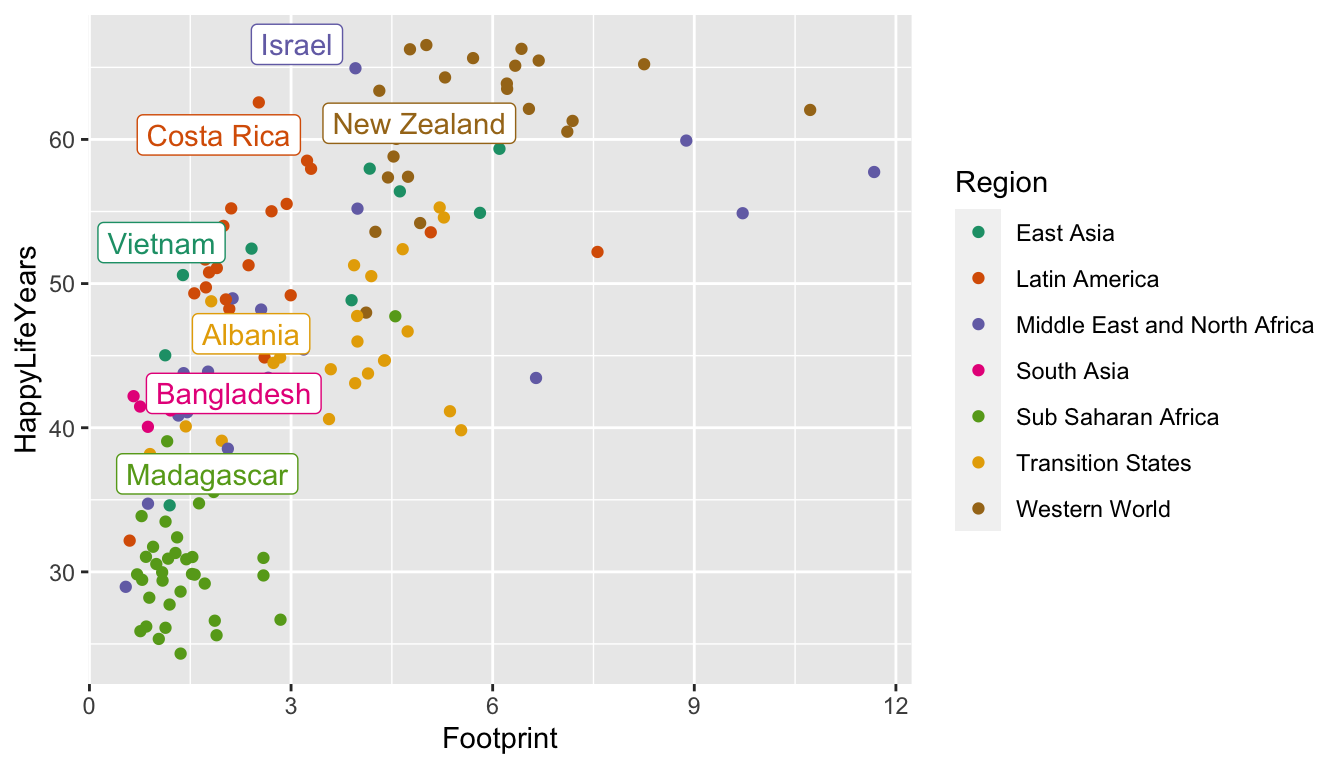
\includegraphics{02-ggplot2_files/figure-latex/unnamed-chunk-16-1.pdf}

What patterns do you see in the scatterplot?

Now, change the x variable from \texttt{Gore} to \texttt{Buchanan}. You should notice something strange in this scatterplot. Try to come up with one explanation for why the outlying point has so many votes for \texttt{Buchanan}.

In trying to come up with an explanation, it would be nice to figure out which Florida county has that outlying point and it would be nice if we knew something about Florida counties. To remedy the first issue, recall that we can type \texttt{View(pres\_df)} to pull up the data set. Once you have the new window open, click on the column heading \texttt{Buchanan} to sort the votes for Buchanan from high to low to figure out which county is the outlier.

Use some Google sleuthing skills to find an explanation: try to search for ``2000 united states presidential election {[}name of outlier county{]}''. Write a sentence about what you find. Hint: if nothing useful pops up, try adding the term ``butterfly ballot'' to your search.

We have used the 2000 Presidential data set to find out something really interesting! In particular, we have used \emph{exploratory data analysis} to examine a data set, without having a specific question of interest that we want to answer. This type of exploring is often really useful, but does have some drawbacks, which we will discuss later in the semester.

\hypertarget{aesthetics-in-aes}{%
\subsection{\texorpdfstring{Aesthetics in \texttt{aes()}}{Aesthetics in aes()}}\label{aesthetics-in-aes}}

For the remainder of this chapter, we will work with some fitness data collected from my Apple Watch since November 2018. The \texttt{higham\_fitness\_clean.csv} contains information on the following variables:

\begin{itemize}
\tightlist
\item
  \texttt{Start}, the month, day, and year that the fitness data was recorded on
\item
  \texttt{month}, the month
\item
  \texttt{weekday}, the day of the week
\item
  \texttt{dayofyear}, the day of the year (so that 304 corresponds to the 304th day of the year)
\item
  \texttt{distance}, distance walked in miles
\item
  \texttt{steps}, the number of steps taken
\item
  \texttt{flights}, the number of flights of stairs climbed
\item
  \texttt{active\_cals}, the number of calories burned from activity
\item
  \texttt{stepgoal}, whether or not I reached 10,000 steps for the day
\item
  \texttt{weekend\_ind}, a variable for whether or not the day of the week was a weekend day (Saturday or Sunday) or a weekday (Monday - Friday).
\end{itemize}

\begin{Shaded}
\begin{Highlighting}[]
\FunctionTok{library}\NormalTok{(tidyverse)}
\NormalTok{fitness\_full }\OtherTok{\textless{}{-}} \FunctionTok{read\_csv}\NormalTok{(}\StringTok{"data/higham\_fitness\_clean.csv"}\NormalTok{) }\SpecialCharTok{\%\textgreater{}\%} \FunctionTok{mutate}\NormalTok{(}\AttributeTok{weekend\_ind =} \FunctionTok{case\_when}\NormalTok{(weekday }\SpecialCharTok{==} \StringTok{"Sat"} \SpecialCharTok{|}\NormalTok{ weekday }\SpecialCharTok{==} \StringTok{"Sun"} \SpecialCharTok{\textasciitilde{}} \StringTok{"weekend"}\NormalTok{,}
  \ConstantTok{TRUE} \SpecialCharTok{\textasciitilde{}} \StringTok{"weekday"}\NormalTok{))}
\CommentTok{\#\textgreater{} }
\CommentTok{\#\textgreater{} {-}{-} Column specification {-}{-}{-}{-}{-}{-}{-}{-}{-}{-}{-}{-}{-}{-}{-}{-}{-}{-}{-}{-}{-}{-}{-}{-}{-}{-}{-}{-}{-}{-}{-}{-}{-}{-}{-}{-}}
\CommentTok{\#\textgreater{} cols(}
\CommentTok{\#\textgreater{}   Start = col\_date(format = ""),}
\CommentTok{\#\textgreater{}   month = col\_character(),}
\CommentTok{\#\textgreater{}   weekday = col\_character(),}
\CommentTok{\#\textgreater{}   dayofyear = col\_double(),}
\CommentTok{\#\textgreater{}   distance = col\_double(),}
\CommentTok{\#\textgreater{}   steps = col\_double(),}
\CommentTok{\#\textgreater{}   flights = col\_double(),}
\CommentTok{\#\textgreater{}   active\_cals = col\_double(),}
\CommentTok{\#\textgreater{}   stepgoal = col\_character()}
\CommentTok{\#\textgreater{} )}
\end{Highlighting}
\end{Shaded}

First, let's make a basic scatterplot to illustrate why it's so important to plot your data. I'll use the variable \texttt{distance} as the x-variable and \texttt{active\_cals} as the y-variable.

\begin{Shaded}
\begin{Highlighting}[]
\FunctionTok{ggplot}\NormalTok{(}\AttributeTok{data =}\NormalTok{ fitness\_full, }\FunctionTok{aes}\NormalTok{(}\AttributeTok{x =}\NormalTok{ distance, }\AttributeTok{y =}\NormalTok{ active\_cals)) }\SpecialCharTok{+}
  \FunctionTok{geom\_point}\NormalTok{()}
\end{Highlighting}
\end{Shaded}

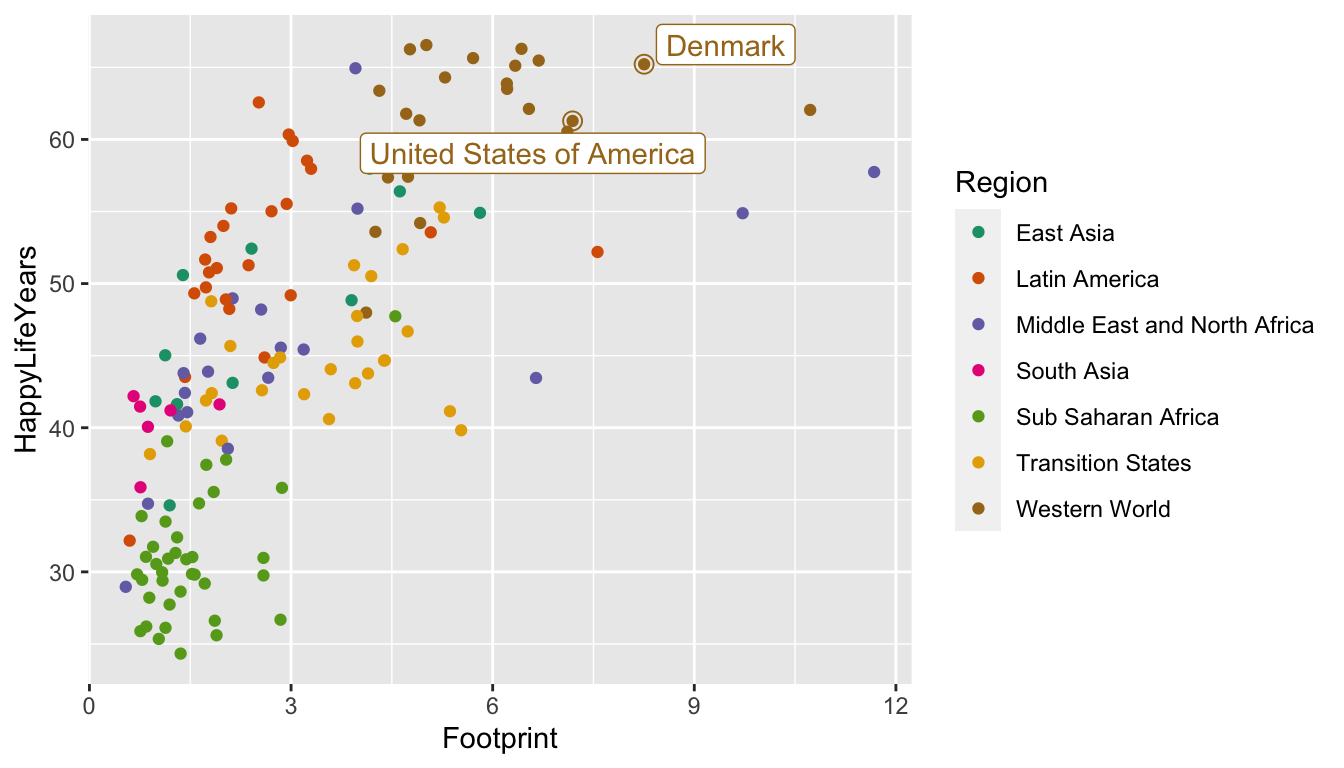
\includegraphics{02-ggplot2_files/figure-latex/unnamed-chunk-18-1.pdf}

One aspect of the plot that you may notice is that there are observations where I burned 0 or very few active calories, yet walked/jogged/ran/moved some distance. Is it possible to not burn any calories and move \textasciitilde{} 4 miles? Probably not, so let's drop these observations from the data set and make a note of why we dropped those observations. Unfortunately, we don't have the tools to do this yet, so just run the following chunk of code without worrying too much about the syntax.

\begin{Shaded}
\begin{Highlighting}[]
\DocumentationTok{\#\# drop observations that have active calories \textless{} 50. }
\DocumentationTok{\#\# assuming that these are data errors or }
\DocumentationTok{\#\# days where the Apple Watch wasn\textquotesingle{}t worn.}
\NormalTok{fitness }\OtherTok{\textless{}{-}}\NormalTok{ fitness\_full }\SpecialCharTok{\%\textgreater{}\%}
  \FunctionTok{filter}\NormalTok{(active\_cals }\SpecialCharTok{\textgreater{}} \DecValTok{50}\NormalTok{)}
\end{Highlighting}
\end{Shaded}

Let's make the plot again with the \texttt{fitness} data set instead of \texttt{fitness\_full} to see if the outliers are actually gone. This time, we will put the \texttt{aes()} in the \texttt{geom\_point()} function:

\begin{Shaded}
\begin{Highlighting}[]
\FunctionTok{ggplot}\NormalTok{(}\AttributeTok{data =}\NormalTok{ fitness) }\SpecialCharTok{+}
  \FunctionTok{geom\_point}\NormalTok{(}\FunctionTok{aes}\NormalTok{(}\AttributeTok{x =}\NormalTok{ distance, }\AttributeTok{y =}\NormalTok{ active\_cals))}
\end{Highlighting}
\end{Shaded}

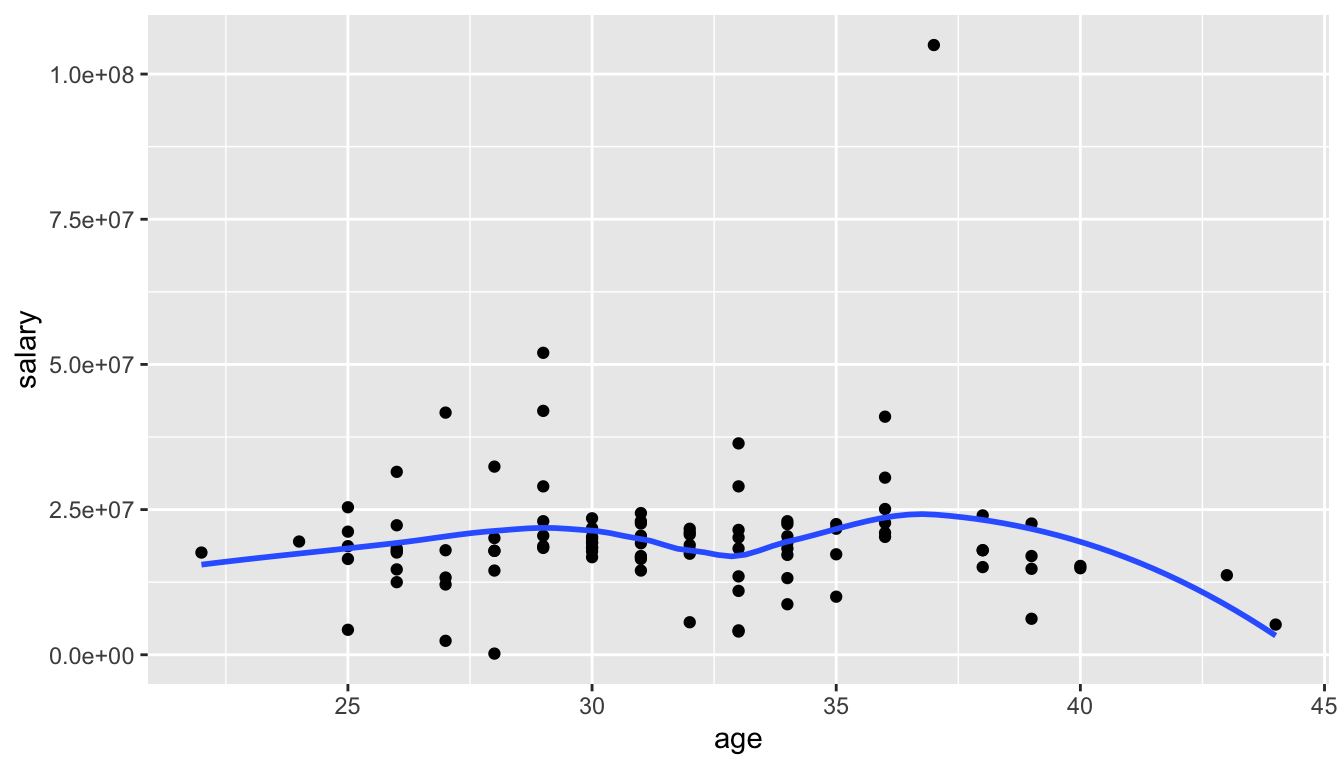
\includegraphics{02-ggplot2_files/figure-latex/unnamed-chunk-20-1.pdf}

Putting the \texttt{aes()} in \texttt{ggplot()} and putting the \texttt{aes()} in \texttt{geom\_point()} results in the same graph in this case. When you put the \texttt{aes()} in \texttt{ggplot()}, \texttt{R} perpetuates these \texttt{aes()} aesthetics in all \texttt{geom\_}s in your plotting command. However, if you put your \texttt{aes()} in \texttt{geom\_point()}, then any future \texttt{geom}s that you use will need you to re-specify different \texttt{aes()}. We'll see an example of this in the exercises.

\textbf{Other \texttt{aes()} Options}

In addition to \texttt{x} and \texttt{y}, we can also use \texttt{aes()} to map variables to things like \texttt{colour}, \texttt{size}, and \texttt{shape}. For example, we might make a scatterplot with \texttt{Start} on the x-axis (for the date) and \texttt{active\_cals} on the y-axis, colouring by whether or not the day of the week was a weekend.

\begin{Shaded}
\begin{Highlighting}[]
\FunctionTok{ggplot}\NormalTok{(}\AttributeTok{data =}\NormalTok{ fitness) }\SpecialCharTok{+}
  \FunctionTok{geom\_point}\NormalTok{(}\FunctionTok{aes}\NormalTok{(}\AttributeTok{x =}\NormalTok{ Start, }\AttributeTok{y =}\NormalTok{ active\_cals, }\AttributeTok{colour =}\NormalTok{ weekend\_ind))}
\end{Highlighting}
\end{Shaded}

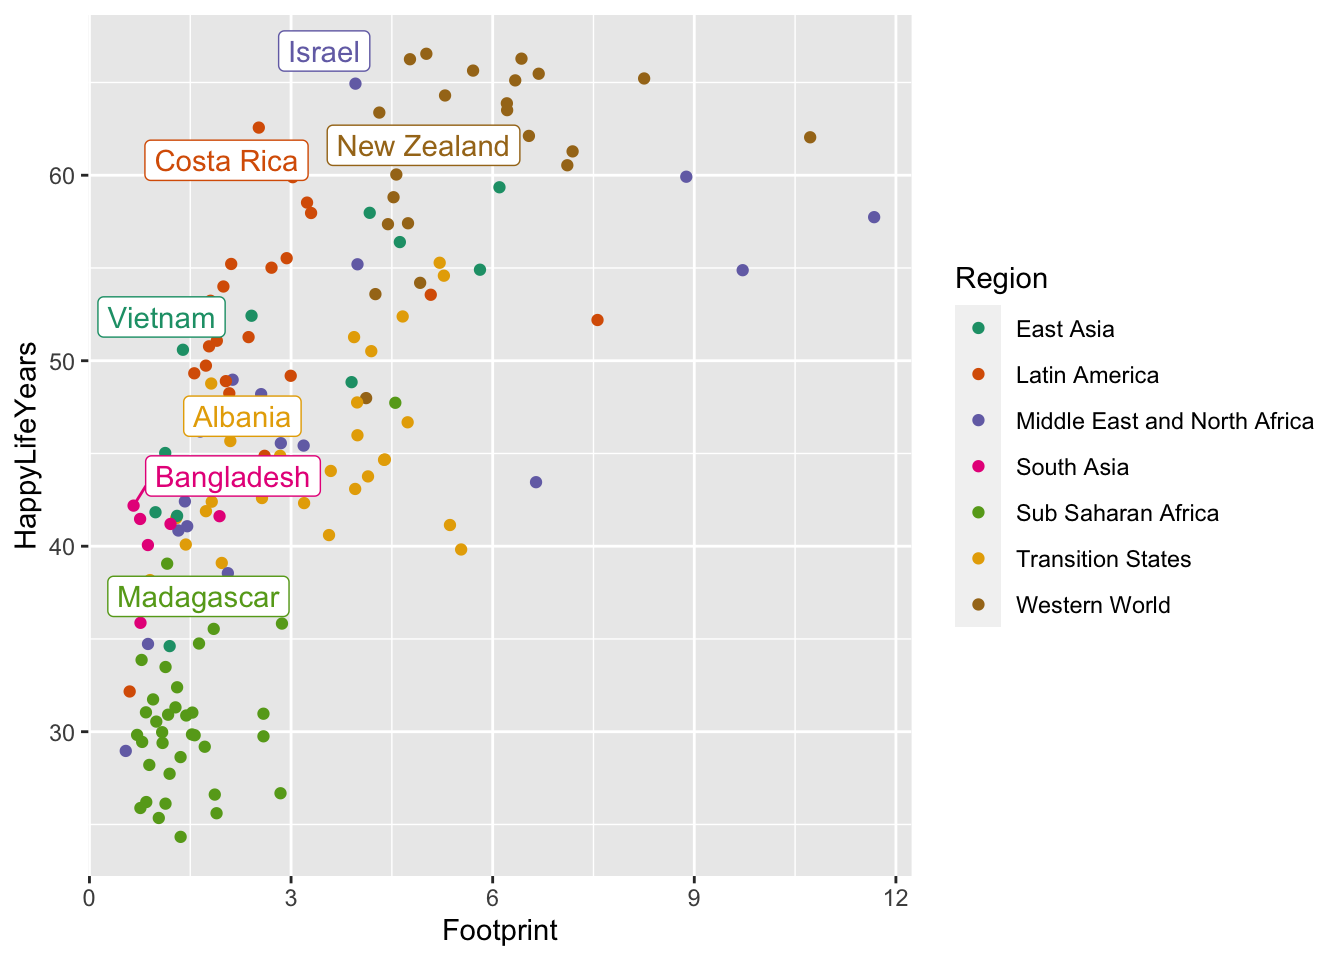
\includegraphics{02-ggplot2_files/figure-latex/unnamed-chunk-21-1.pdf}

Is there anything useful that you notice about the plot? Is there anything about the plot that could be improved?

Instead of using colour, you can also specify the point shape. This could be useful, for example, if you are printing something in black and white.

\begin{Shaded}
\begin{Highlighting}[]
\FunctionTok{ggplot}\NormalTok{(}\AttributeTok{data =}\NormalTok{ fitness) }\SpecialCharTok{+}
  \FunctionTok{geom\_point}\NormalTok{(}\FunctionTok{aes}\NormalTok{(}\AttributeTok{x =}\NormalTok{ Start, }\AttributeTok{y =}\NormalTok{ active\_cals, }\AttributeTok{shape =}\NormalTok{ weekend\_ind))}
\end{Highlighting}
\end{Shaded}

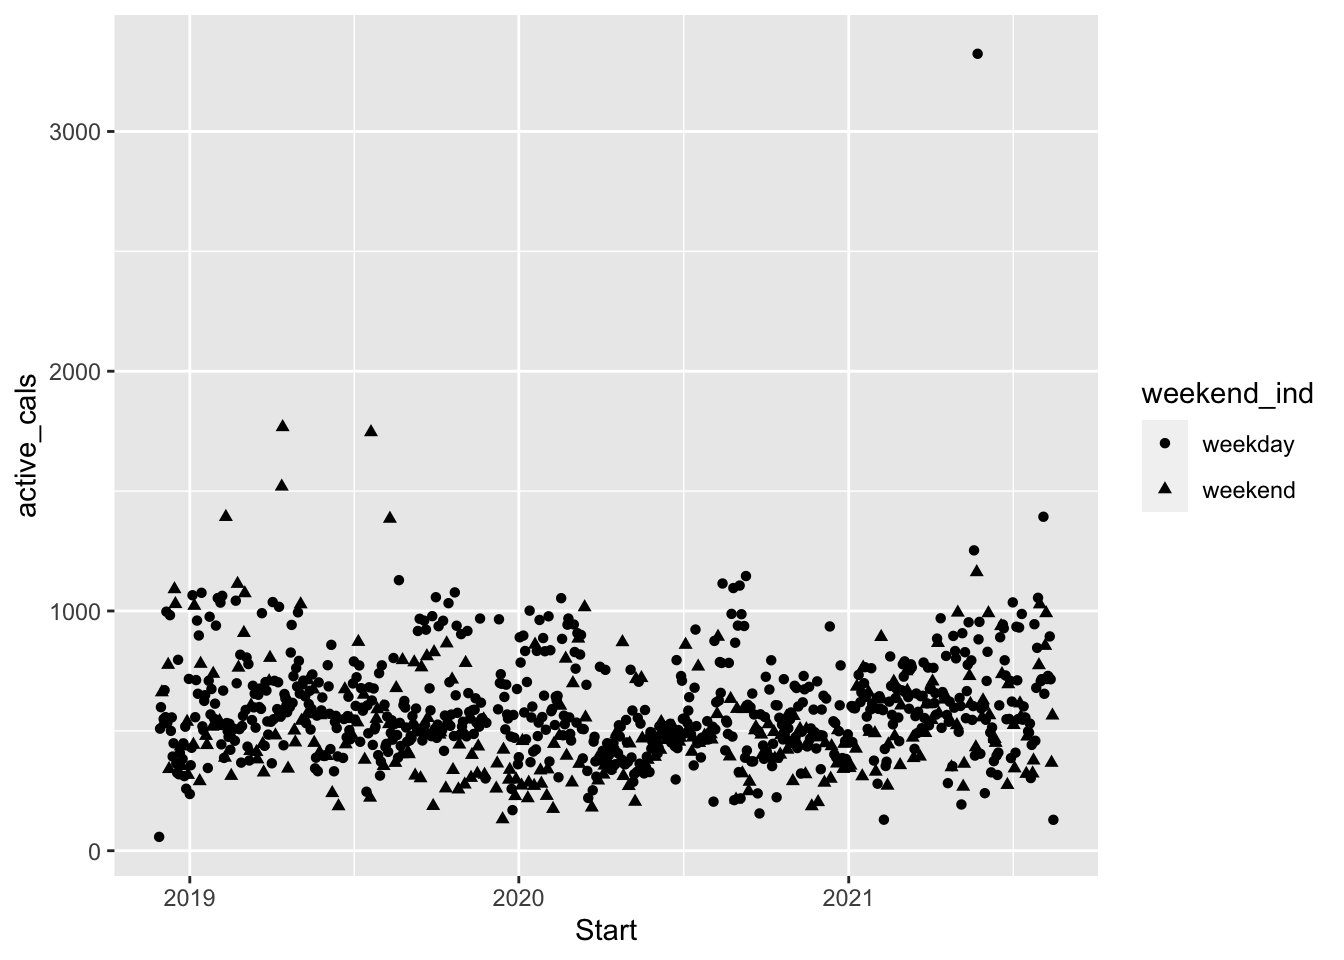
\includegraphics{02-ggplot2_files/figure-latex/unnamed-chunk-22-1.pdf}

Do you prefer the colour or the shape? Why?

Finally, another common \texttt{aes()} is \texttt{size}. For example, we could make the size of the points in the scatterplot change depending on how many \texttt{flights} of stairs I climbed.

\begin{Shaded}
\begin{Highlighting}[]
\FunctionTok{ggplot}\NormalTok{(}\AttributeTok{data =}\NormalTok{ fitness) }\SpecialCharTok{+}
  \FunctionTok{geom\_point}\NormalTok{(}\FunctionTok{aes}\NormalTok{(}\AttributeTok{x =}\NormalTok{ Start, }\AttributeTok{y =}\NormalTok{ active\_cals, }\AttributeTok{size =}\NormalTok{ flights))}
\end{Highlighting}
\end{Shaded}

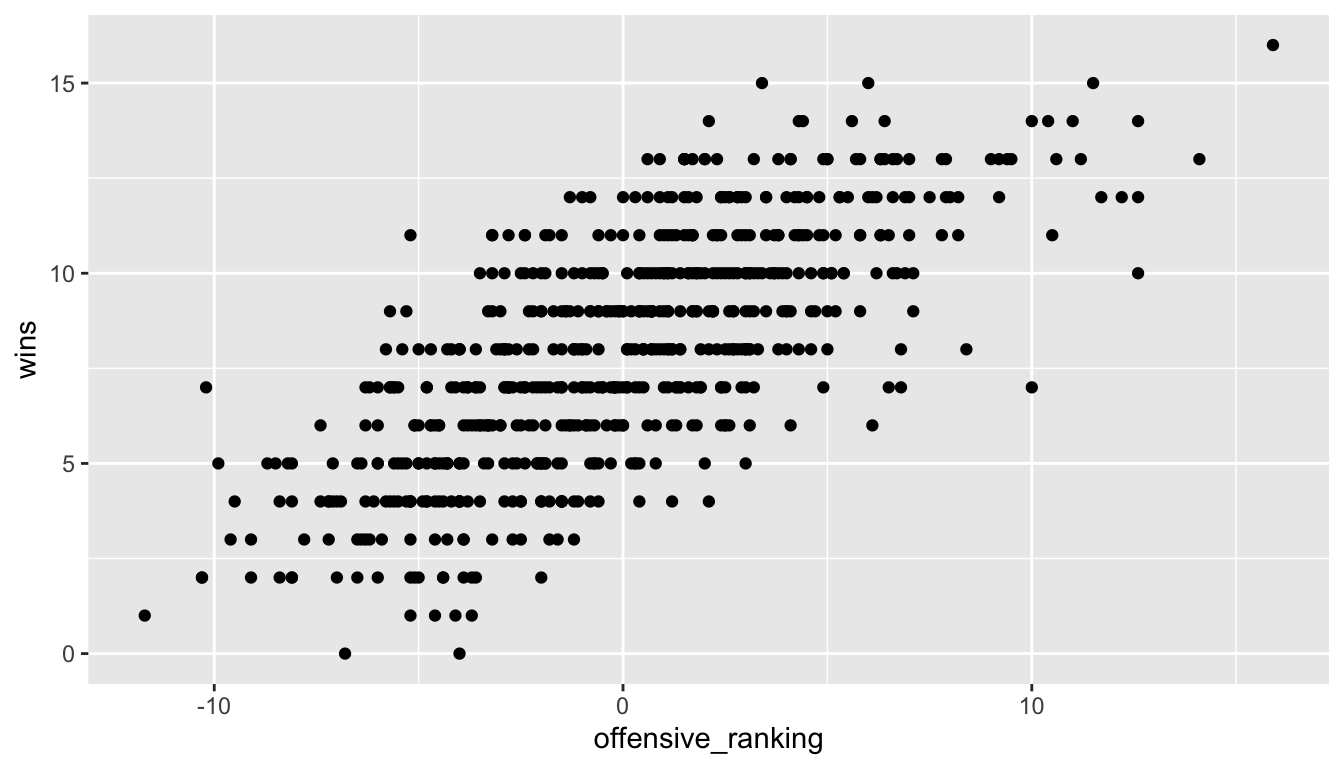
\includegraphics{02-ggplot2_files/figure-latex/unnamed-chunk-23-1.pdf}

I don't think any of the previous three plots are necessarily the ``best'' and need some work, but, part of the fun of exploratory data analysis is making trying out different plots to see what ``works.''

\textbf{Inside vs Outside \texttt{aes()}}

We've changed the colour of the points to correspond to \texttt{weekend\_ind}, but what if we just wanted to change the colour of points to all be the same colour, \texttt{"purple"}. Try running the following code chunk:

\begin{Shaded}
\begin{Highlighting}[]
\FunctionTok{ggplot}\NormalTok{(}\AttributeTok{data =}\NormalTok{ fitness) }\SpecialCharTok{+}
  \FunctionTok{geom\_point}\NormalTok{(}\FunctionTok{aes}\NormalTok{(}\AttributeTok{x =}\NormalTok{ Start, }\AttributeTok{y =}\NormalTok{ active\_cals, }\AttributeTok{colour =} \StringTok{"purple"}\NormalTok{))}
\end{Highlighting}
\end{Shaded}

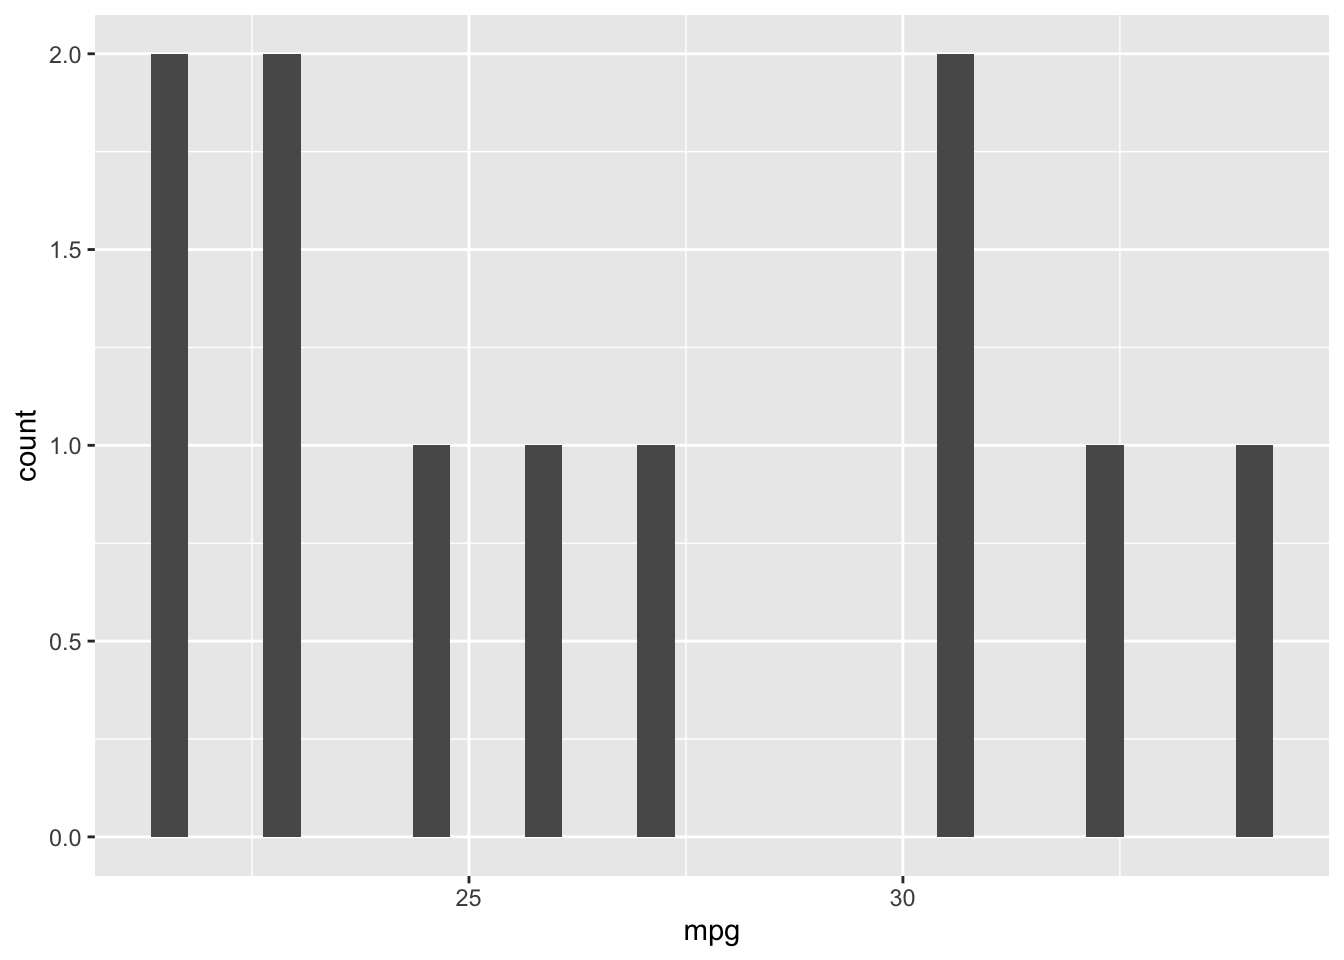
\includegraphics{02-ggplot2_files/figure-latex/unnamed-chunk-24-1.pdf}

What does the graph look like? Did it do what you expected?

Putting \texttt{colour\ =\ \_\_\_\_} inside \texttt{aes()} or outside \texttt{aes()} achieves different things. In general,

\begin{itemize}
\item
  when we want to map something in our data set (\texttt{fitness}) to something in our plot (\texttt{x}, \texttt{y}, \texttt{colour}, \texttt{size}, etc.), we put that \textbf{inside} the \texttt{aes()} as in \texttt{geom\_point(aes(colour\ =\ weekend\_ind))}.
\item
  When we assign fixed characteristics that don't come from the data, we put them \textbf{outside} the \texttt{aes()}, as in \texttt{geom\_point(colour\ =\ "purple")}.
\end{itemize}

You can also change the overall point size and shape. The standard size is \texttt{1} so the following code chunk makes the points bigger. The standard shape is \texttt{19}: you can try changing that to other integers to see what other shapes you can get.

\begin{Shaded}
\begin{Highlighting}[]
\FunctionTok{ggplot}\NormalTok{(}\AttributeTok{data =}\NormalTok{ fitness) }\SpecialCharTok{+}
  \FunctionTok{geom\_point}\NormalTok{(}\FunctionTok{aes}\NormalTok{(}\AttributeTok{x =}\NormalTok{ Start, }\AttributeTok{y =}\NormalTok{ active\_cals), }\AttributeTok{size =} \FloatTok{1.5}\NormalTok{, }\AttributeTok{shape =} \DecValTok{19}\NormalTok{)}
\end{Highlighting}
\end{Shaded}

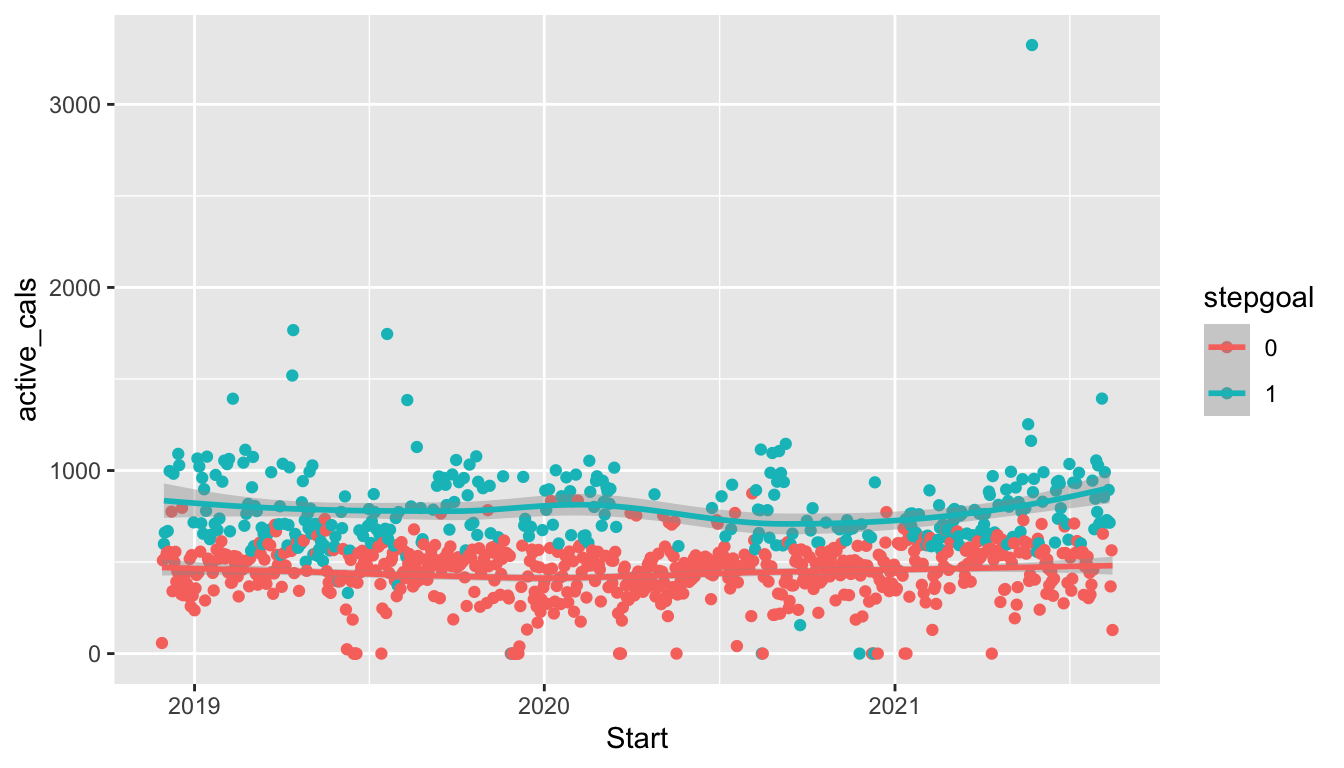
\includegraphics{02-ggplot2_files/figure-latex/unnamed-chunk-25-1.pdf}

\hypertarget{using-more-than-one-geom}{%
\subsection{\texorpdfstring{Using More Than One \texttt{geom()}}{Using More Than One geom()}}\label{using-more-than-one-geom}}

We might also be interested in fitting a smooth curve to our scatterplot. When we want to put more than one ``geom'' on our plot, we can use multiple \texttt{geoms}. Since I want the \texttt{aes()} to apply to \textbf{both} \texttt{geom\_point()} and \texttt{geom\_smooth()}, I am going to move the \texttt{aes()} command to the overall \texttt{ggplot()} line of code:

\begin{Shaded}
\begin{Highlighting}[]
\FunctionTok{ggplot}\NormalTok{(}\AttributeTok{data =}\NormalTok{ fitness, }\FunctionTok{aes}\NormalTok{(}\AttributeTok{x =}\NormalTok{ Start, }\AttributeTok{y =}\NormalTok{ active\_cals)) }\SpecialCharTok{+}
  \FunctionTok{geom\_point}\NormalTok{() }\SpecialCharTok{+}
  \FunctionTok{geom\_smooth}\NormalTok{()}
\CommentTok{\#\textgreater{} \textasciigrave{}geom\_smooth()\textasciigrave{} using method = \textquotesingle{}loess\textquotesingle{} and formula \textquotesingle{}y \textasciitilde{} x\textquotesingle{}}
\end{Highlighting}
\end{Shaded}

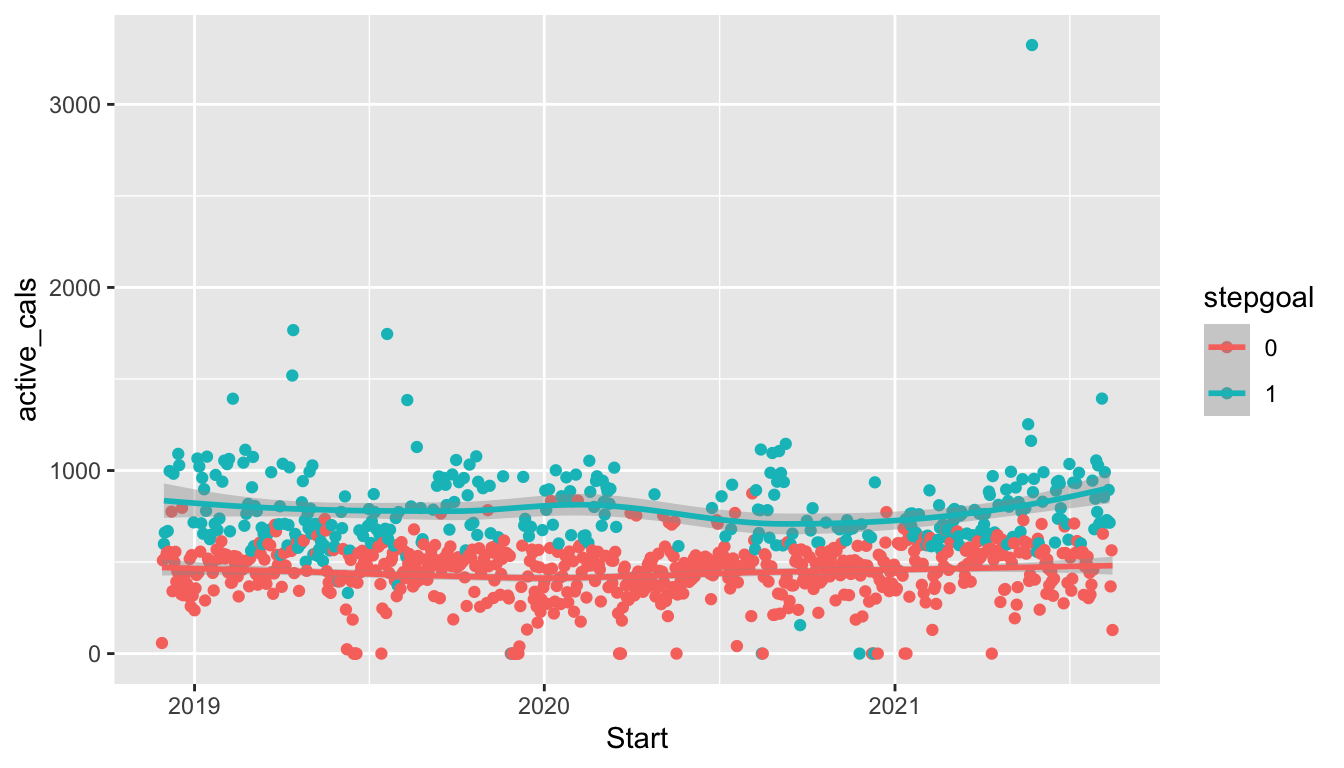
\includegraphics{02-ggplot2_files/figure-latex/unnamed-chunk-26-1.pdf}

Within \texttt{geom\_smooth()}, you can set \texttt{se\ =\ FALSE} to get rid of the grey standard errors around each of the lines, and you can set\texttt{method\ =\ "lm"} to fit straight linear regression lines instead of smooth curves:

\begin{Shaded}
\begin{Highlighting}[]
\FunctionTok{ggplot}\NormalTok{(}\AttributeTok{data =}\NormalTok{ fitness, }\FunctionTok{aes}\NormalTok{(}\AttributeTok{x =}\NormalTok{ Start, }\AttributeTok{y =}\NormalTok{ active\_cals)) }\SpecialCharTok{+}
  \FunctionTok{geom\_point}\NormalTok{() }\SpecialCharTok{+}
  \FunctionTok{geom\_smooth}\NormalTok{(}\AttributeTok{se =} \ConstantTok{FALSE}\NormalTok{, }\AttributeTok{method =} \StringTok{"lm"}\NormalTok{)}
\CommentTok{\#\textgreater{} \textasciigrave{}geom\_smooth()\textasciigrave{} using formula \textquotesingle{}y \textasciitilde{} x\textquotesingle{}}
\end{Highlighting}
\end{Shaded}

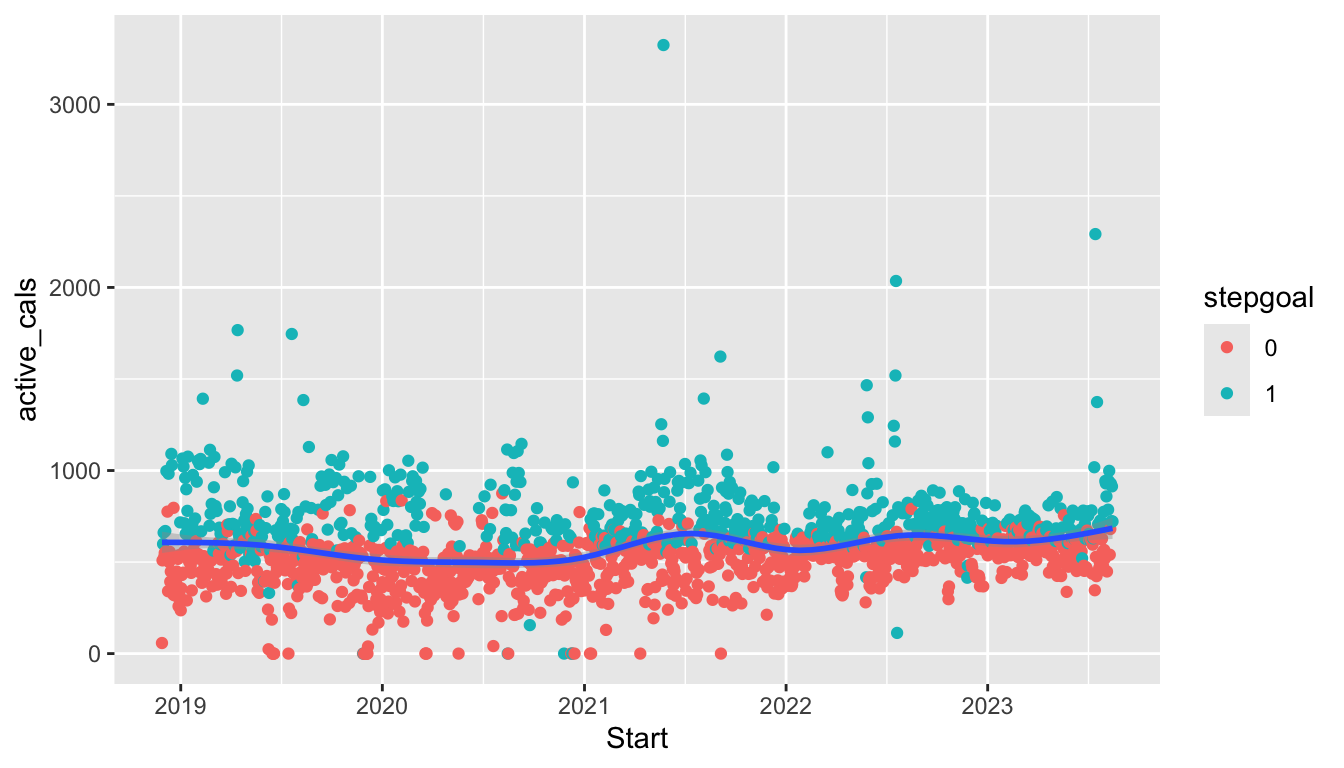
\includegraphics{02-ggplot2_files/figure-latex/unnamed-chunk-27-1.pdf}

Does it look like there is an increasing overall trend? decreasing? Does it make sense to use a line to model the relationship or did you prefer the smooth curve?

\hypertarget{line-plots-with-geom_line}{%
\subsection{\texorpdfstring{Line Plots with \texttt{geom\_line()}}{Line Plots with geom\_line()}}\label{line-plots-with-geom_line}}

Line plots are often useful when you have a quantitative variable that you'd like to explore over time. The y-axis is the quantitative variable while the x-axis is typically time. More generally, line plots are often used when the x-axis variable has one discrete value for each y-axis variable. For example, suppose we want to explore how my step count has changed through time over the past couple of years. Compare the standard scatterplot with the following line plot: which do you prefer?

\begin{Shaded}
\begin{Highlighting}[]
\FunctionTok{ggplot}\NormalTok{(}\AttributeTok{data =}\NormalTok{ fitness, }\AttributeTok{mapping =} \FunctionTok{aes}\NormalTok{(}\AttributeTok{x =}\NormalTok{ Start, }\AttributeTok{y =}\NormalTok{ steps)) }\SpecialCharTok{+}
  \FunctionTok{geom\_point}\NormalTok{() }\SpecialCharTok{+} \FunctionTok{geom\_smooth}\NormalTok{() }\SpecialCharTok{+} \FunctionTok{xlab}\NormalTok{(}\StringTok{"Date"}\NormalTok{)}
\CommentTok{\#\textgreater{} \textasciigrave{}geom\_smooth()\textasciigrave{} using method = \textquotesingle{}loess\textquotesingle{} and formula \textquotesingle{}y \textasciitilde{} x\textquotesingle{}}
\end{Highlighting}
\end{Shaded}

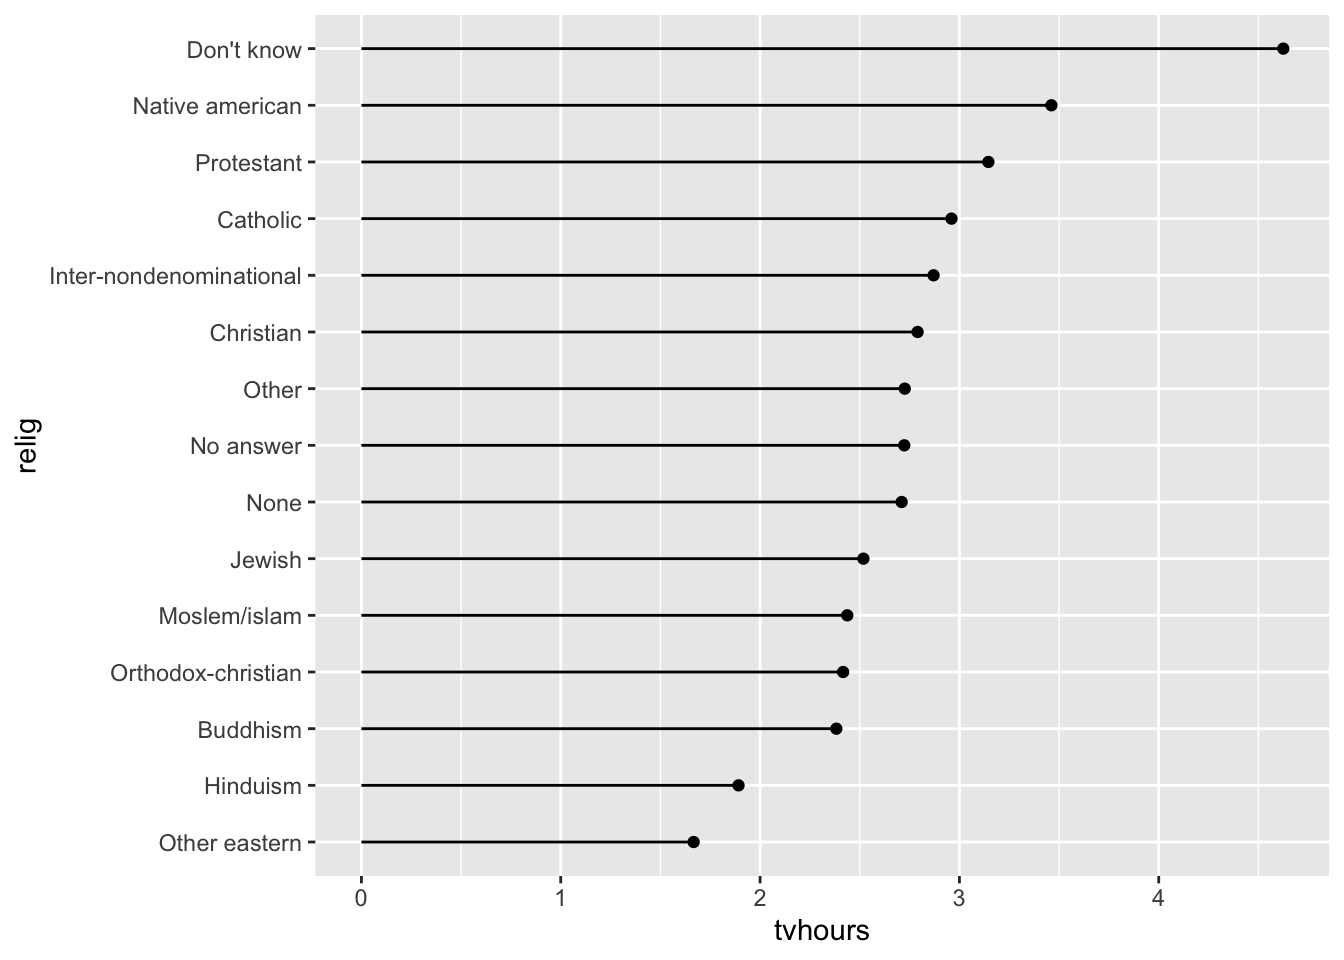
\includegraphics{02-ggplot2_files/figure-latex/unnamed-chunk-28-1.pdf}

\begin{Shaded}
\begin{Highlighting}[]
\FunctionTok{ggplot}\NormalTok{(}\AttributeTok{data =}\NormalTok{ fitness, }\AttributeTok{mapping =} \FunctionTok{aes}\NormalTok{(}\AttributeTok{x =}\NormalTok{ Start, }\AttributeTok{y =}\NormalTok{ steps)) }\SpecialCharTok{+}
  \FunctionTok{geom\_line}\NormalTok{() }\SpecialCharTok{+} \FunctionTok{geom\_smooth}\NormalTok{() }\SpecialCharTok{+} \FunctionTok{xlab}\NormalTok{(}\StringTok{"Date"}\NormalTok{)}
\CommentTok{\#\textgreater{} \textasciigrave{}geom\_smooth()\textasciigrave{} using method = \textquotesingle{}loess\textquotesingle{} and formula \textquotesingle{}y \textasciitilde{} x\textquotesingle{}}
\end{Highlighting}
\end{Shaded}

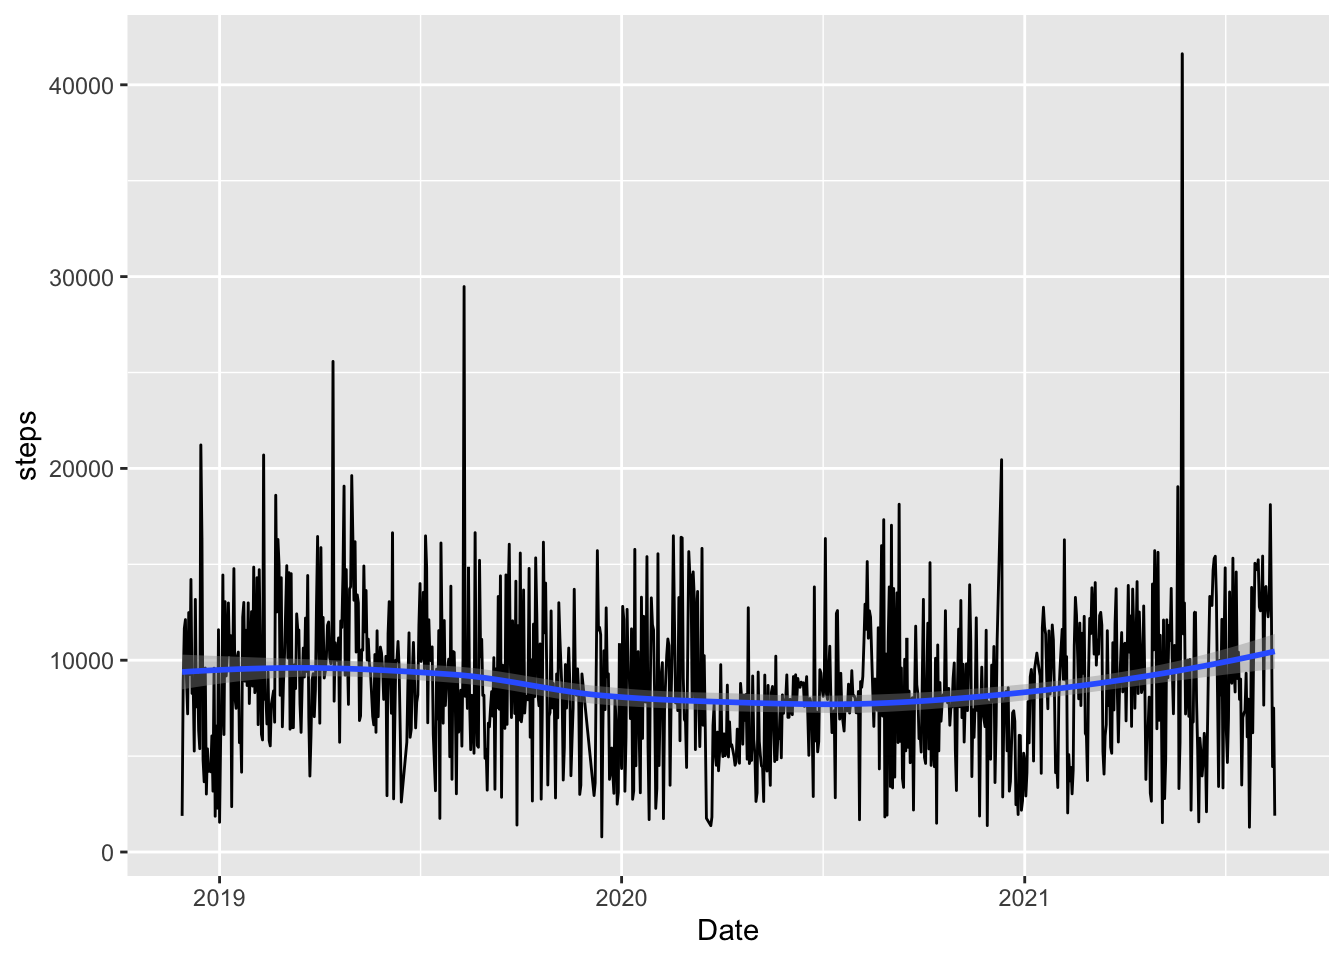
\includegraphics{02-ggplot2_files/figure-latex/unnamed-chunk-28-2.pdf}

Can you spot the start of the pandemic in the graph? What seemed to happen with the step count?

\hypertarget{faceting}{%
\subsection{Faceting}\label{faceting}}

Using colour to colour points of different levels of a categorical variable is generally fine when there are just a couple of levels and/or there is little overlap among the levels. But, what if there are a lot more than two categories to colour by. For example, let's move back to the STAT 113 survey data set and investigate the relationship between \texttt{Pulse} and \texttt{Exercise} for different class \texttt{Year}'s. We might hypothesize that students who get more exercise tend to have lower pulse rates.

\begin{Shaded}
\begin{Highlighting}[]
\FunctionTok{ggplot}\NormalTok{(}\AttributeTok{data =}\NormalTok{ stat113\_df, }\FunctionTok{aes}\NormalTok{(}\AttributeTok{x =}\NormalTok{ Exercise, }\AttributeTok{y =}\NormalTok{ Pulse,}
                           \AttributeTok{colour =}\NormalTok{ Year)) }\SpecialCharTok{+}
  \FunctionTok{geom\_point}\NormalTok{() }\SpecialCharTok{+}
  \FunctionTok{geom\_smooth}\NormalTok{(}\AttributeTok{se =} \ConstantTok{TRUE}\NormalTok{)}
\CommentTok{\#\textgreater{} \textasciigrave{}geom\_smooth()\textasciigrave{} using method = \textquotesingle{}loess\textquotesingle{} and formula \textquotesingle{}y \textasciitilde{} x\textquotesingle{}}
\CommentTok{\#\textgreater{} Warning: Removed 40 rows containing non{-}finite values}
\CommentTok{\#\textgreater{} (stat\_smooth).}
\CommentTok{\#\textgreater{} Warning: Removed 40 rows containing missing values}
\CommentTok{\#\textgreater{} (geom\_point).}
\end{Highlighting}
\end{Shaded}

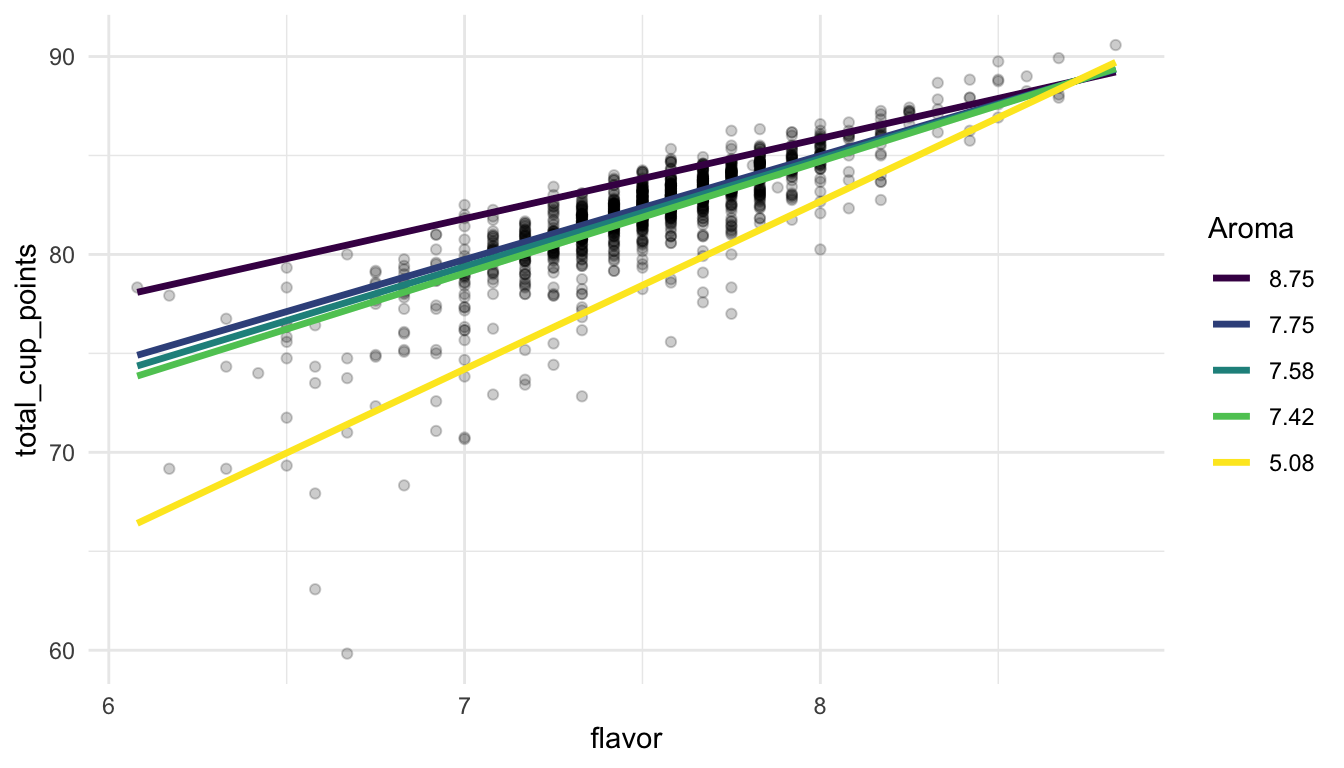
\includegraphics{02-ggplot2_files/figure-latex/unnamed-chunk-29-1.pdf}

When there are many different categories for a categorical variable (there are only 4 categories for \texttt{Year}, but this particular plot is still a bit difficult to read), it can sometimes be useful to \texttt{facet} the plot by that variable instead of trying to use different \texttt{colour}s or \texttt{shape}s.

\begin{Shaded}
\begin{Highlighting}[]
\FunctionTok{ggplot}\NormalTok{(}\AttributeTok{data =}\NormalTok{ stat113\_df, }\FunctionTok{aes}\NormalTok{(}\AttributeTok{x =}\NormalTok{ Exercise, }\AttributeTok{y =}\NormalTok{ Pulse)) }\SpecialCharTok{+}
  \FunctionTok{geom\_point}\NormalTok{() }\SpecialCharTok{+}
  \FunctionTok{geom\_smooth}\NormalTok{(}\AttributeTok{se =} \ConstantTok{TRUE}\NormalTok{) }\SpecialCharTok{+}
  \FunctionTok{facet\_wrap}\NormalTok{(}\SpecialCharTok{\textasciitilde{}}\NormalTok{ Year)}
\CommentTok{\#\textgreater{} \textasciigrave{}geom\_smooth()\textasciigrave{} using method = \textquotesingle{}loess\textquotesingle{} and formula \textquotesingle{}y \textasciitilde{} x\textquotesingle{}}
\CommentTok{\#\textgreater{} Warning: Removed 40 rows containing non{-}finite values}
\CommentTok{\#\textgreater{} (stat\_smooth).}
\CommentTok{\#\textgreater{} Warning: Removed 40 rows containing missing values}
\CommentTok{\#\textgreater{} (geom\_point).}
\end{Highlighting}
\end{Shaded}

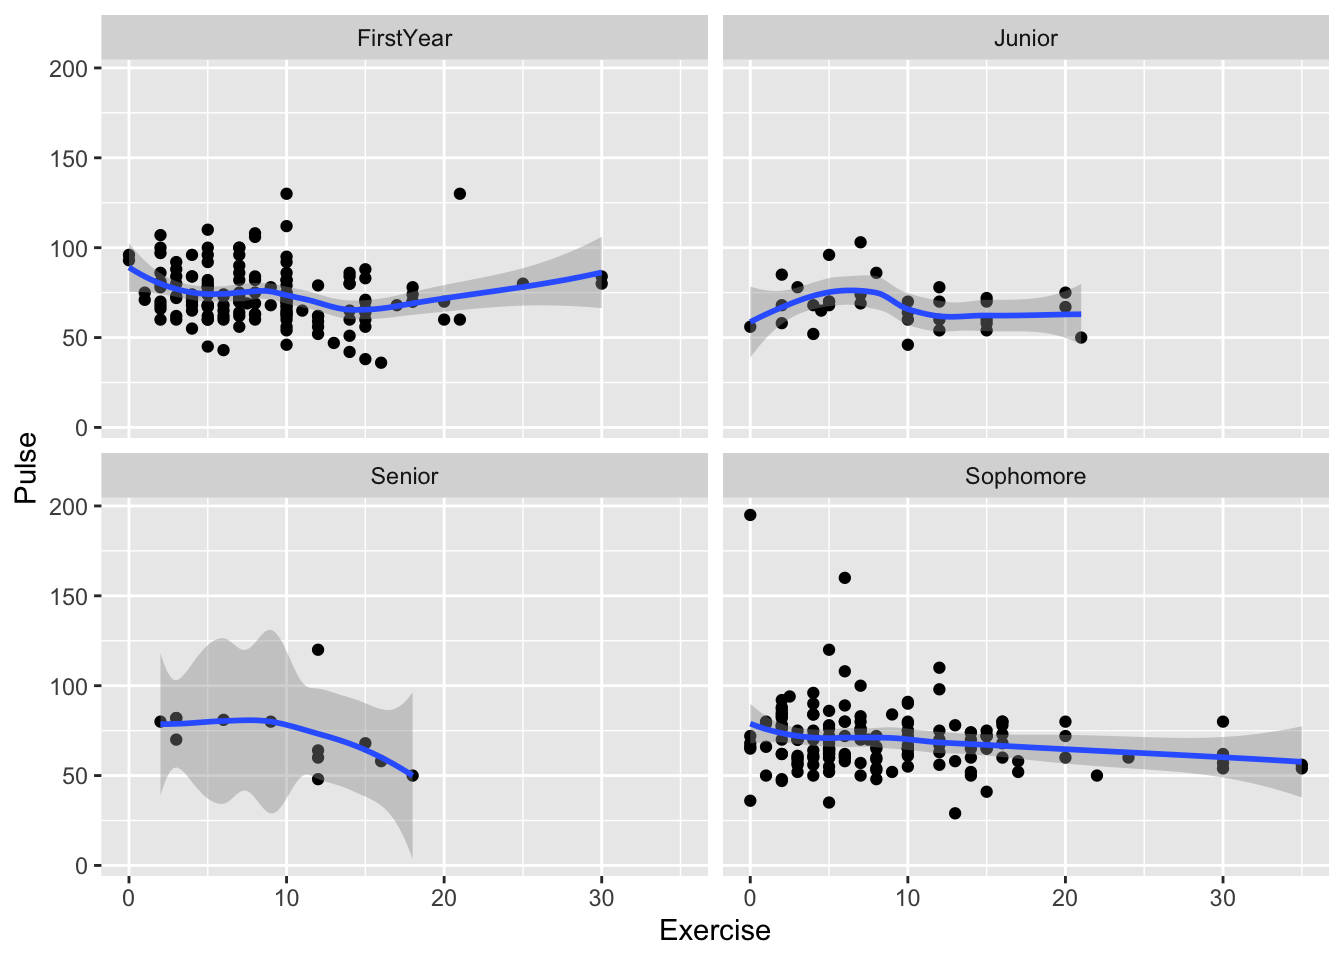
\includegraphics{02-ggplot2_files/figure-latex/unnamed-chunk-30-1.pdf}

We have eliminated the \texttt{colour\ =} argument and added \texttt{facet\_wrap(\ \textasciitilde{}\ name\_of\_facet\_variable)}. Doing so creates a different scatterplot and smooth line for each level of \texttt{name\_of\_facet\_variable}.

What can you see from this plot that was harder to see from the plot with colour?

Does the data seem to support the hypothesis that more exercise is associated with lower pulse rates in this sample of students?

\hypertarget{exercise-2-2}{%
\subsection{Exercises}\label{exercise-2-2}}

Exercises marked with an * indicate that the exercise has a solution at the end of the chapter at \ref{solutions-2}.

\begin{enumerate}
\def\labelenumi{\arabic{enumi}.}
\item
  Fix the code chunk where we tried to specify the colour of all points to be purple to actually make all of the points ``purple'' by moving \texttt{colour\ =\ "purple"} outside the parentheses in \texttt{aes()} (but still inside \texttt{geom\_point()}).
\item
  In the console (bottom-left) window, type \texttt{?geom\_smooth} and scroll down to ``Arguments.'' Find \texttt{span}, read about it, and then, within the \texttt{geom\_smooth()} argument of the line plot with steps vs.~date, add a \texttt{span} argument to make the smooth line wigglier.
\item
  Explain why it doesn't make sense to construct a line plot of \texttt{Exercise} vs.~\texttt{GPA}.
\item
  * Make a scatterplot of \texttt{Hgt} on the y-axis and \texttt{Wgt} on the x-axis, colouring by \texttt{Sport}. Add a smooth fitted curve to your scatterplot. Then, move \texttt{colour\ =\ Sport} from an \texttt{aes()} in the \texttt{ggplot()} function to an \texttt{aes()} in the \texttt{geom\_point()} function. What changes in the plot? Can you give an explanation as to why that change occurs?
\item
  * Faceting can be used for other types of plots too! Make a pair of faceted histograms for a quantitative variable of your choosing that are faceted by a categorical variable of your choosing.
\end{enumerate}

\hypertarget{boxplots-stacked-barplots-and-others}{%
\section{Boxplots, Stacked Barplots and Others}\label{boxplots-stacked-barplots-and-others}}

There are a few other common geoms that will be useful throughout the semester. These only skim the surface: we'll come back to plotting in a few weeks, after we're able to do more with data wrangling and reshaping.

\hypertarget{graphing-a-quant.-variable-vs.-a-cat.-variable}{%
\subsection{Graphing a Quant. Variable vs.~a Cat. Variable}\label{graphing-a-quant.-variable-vs.-a-cat.-variable}}

Another common plot used in Intro Stat courses is a boxplot. Side-by-side boxplots are particularly useful if you want to compare a quantitative response variable across two or more levels of a categorical variable. Let's stick with the STAT 113 survey data to examine the relationship between \texttt{Exercise} and \texttt{Award} preference.

\begin{Shaded}
\begin{Highlighting}[]
\FunctionTok{ggplot}\NormalTok{(}\AttributeTok{data =}\NormalTok{ stat113\_df, }\FunctionTok{aes}\NormalTok{(}\AttributeTok{x =}\NormalTok{ Award, }\AttributeTok{y =}\NormalTok{ Exercise)) }\SpecialCharTok{+}
  \FunctionTok{geom\_boxplot}\NormalTok{()}
\CommentTok{\#\textgreater{} Warning: Removed 7 rows containing non{-}finite values}
\CommentTok{\#\textgreater{} (stat\_boxplot).}
\end{Highlighting}
\end{Shaded}

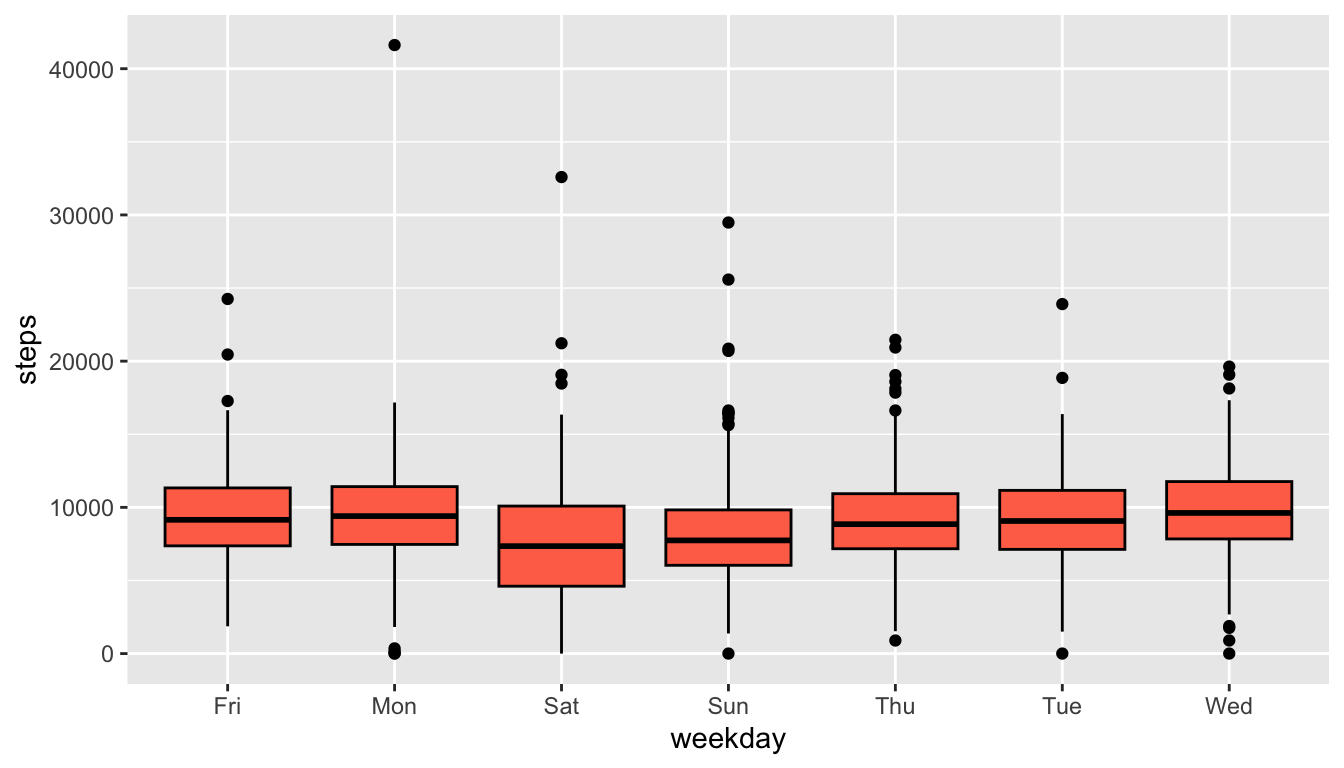
\includegraphics{02-ggplot2_files/figure-latex/unnamed-chunk-31-1.pdf}

What can you conclude from the plot?

An alternative to side-by-side boxplots are violin plots:

\begin{Shaded}
\begin{Highlighting}[]
\FunctionTok{ggplot}\NormalTok{(}\AttributeTok{data =}\NormalTok{ stat113\_df, }\FunctionTok{aes}\NormalTok{(}\AttributeTok{x =}\NormalTok{ Award, }\AttributeTok{y =}\NormalTok{ Exercise)) }\SpecialCharTok{+}
  \FunctionTok{geom\_violin}\NormalTok{()}
\CommentTok{\#\textgreater{} Warning: Removed 7 rows containing non{-}finite values}
\CommentTok{\#\textgreater{} (stat\_ydensity).}
\end{Highlighting}
\end{Shaded}

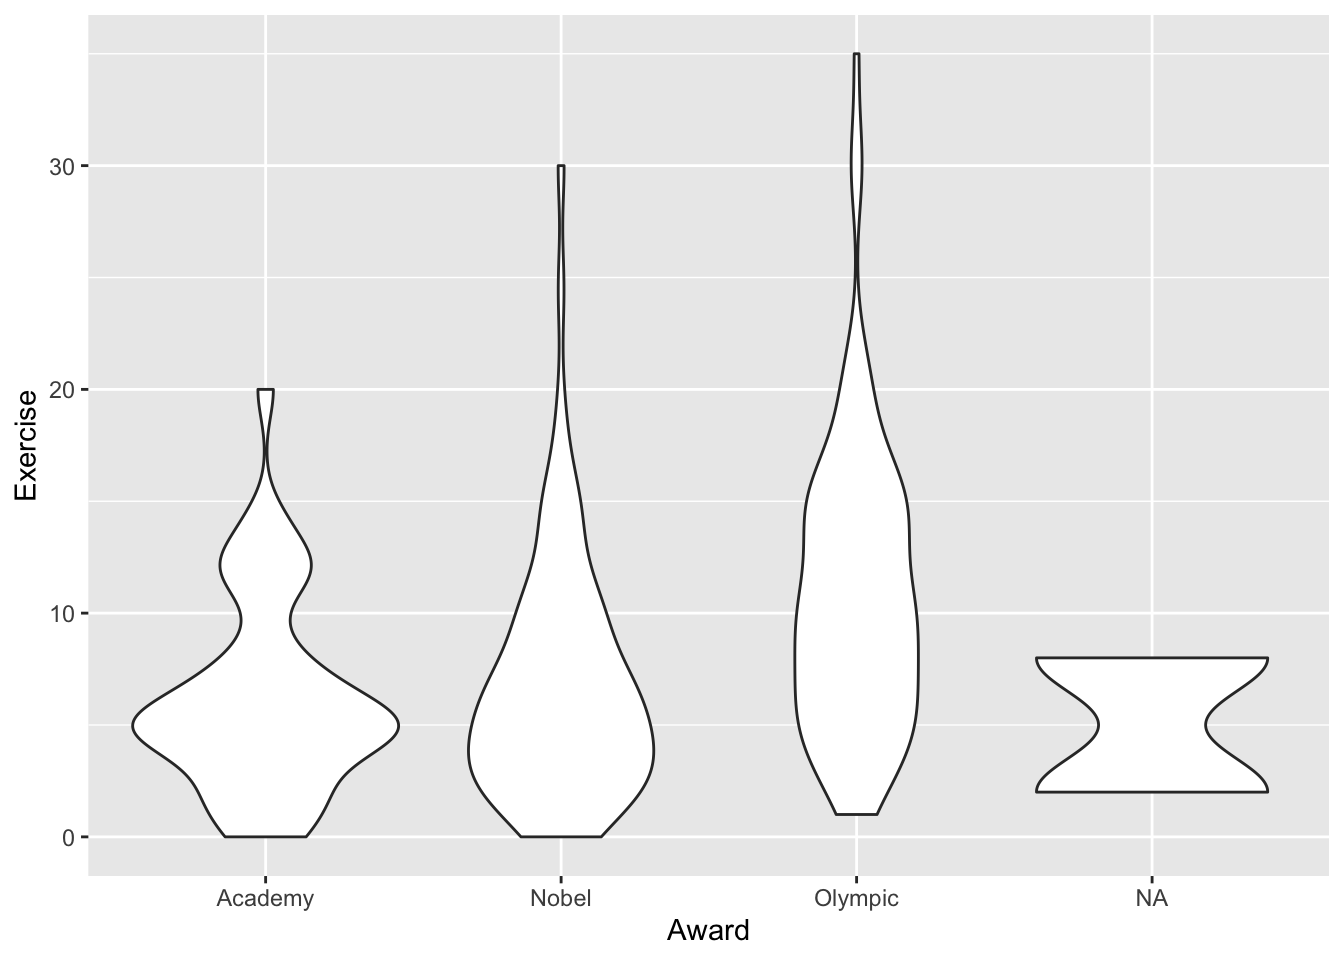
\includegraphics{02-ggplot2_files/figure-latex/unnamed-chunk-32-1.pdf}

Read about Violin plots by typing \texttt{?geom\_violin} into your console (bottom-left window). How are they different than boxplots?

\hypertarget{graphing-two-categorical-variables}{%
\subsection{Graphing Two Categorical Variables}\label{graphing-two-categorical-variables}}

The only combination of two variables that we have yet to explore are two variables that are both categorical. Let's look at the relationship between \texttt{Year} and \texttt{SocialMedia} first using a stacked bar plot.

To make the graph, we specify \texttt{position\ =\ "fill"} so that the bars are ``filled'' by \texttt{stepgoal}.

\begin{Shaded}
\begin{Highlighting}[]
\FunctionTok{ggplot}\NormalTok{(}\AttributeTok{data =}\NormalTok{ stat113\_df, }\FunctionTok{aes}\NormalTok{(}\AttributeTok{x =}\NormalTok{ Year, }\AttributeTok{fill =}\NormalTok{ SocialMedia)) }\SpecialCharTok{+}
  \FunctionTok{geom\_bar}\NormalTok{(}\AttributeTok{position =} \StringTok{"fill"}\NormalTok{) }\SpecialCharTok{+}
  \FunctionTok{ylab}\NormalTok{(}\StringTok{"Proportion"}\NormalTok{)}
\end{Highlighting}
\end{Shaded}

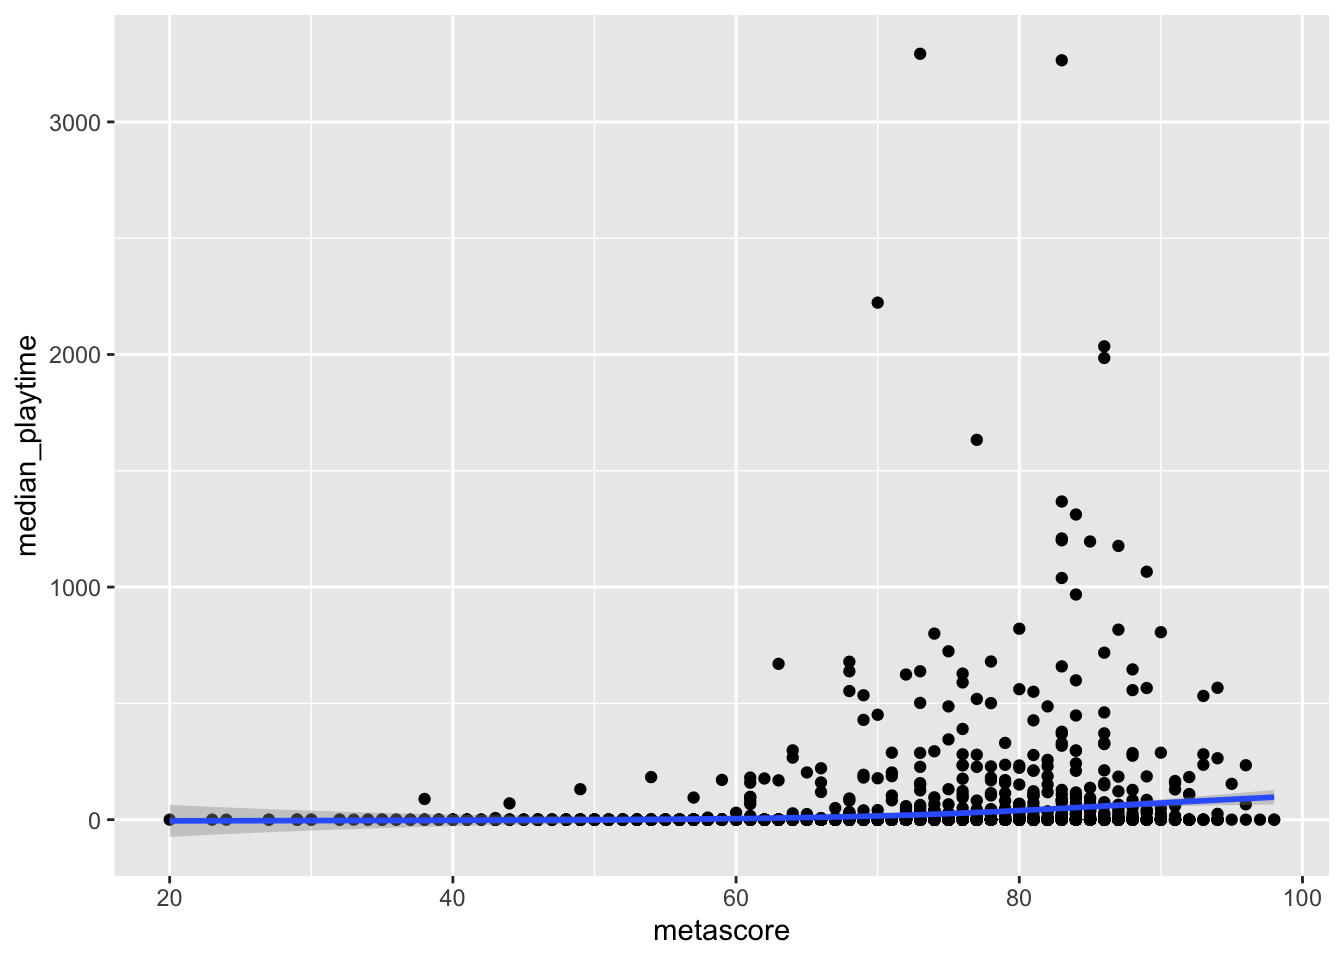
\includegraphics{02-ggplot2_files/figure-latex/unnamed-chunk-33-1.pdf}

What patterns do you notice from the plot? Is there anything about the plot that could be improved?

\hypertarget{exercise-2-3}{%
\subsection{Exercises}\label{exercise-2-3}}

Exercises marked with an * indicate that the exercise has a solution at the end of the chapter at \ref{solutions-2}.

\begin{enumerate}
\def\labelenumi{\arabic{enumi}.}
\item
  * Change the colour of the inside of the boxplots in the Exercise vs.~Award graph to be \texttt{"blue"}. Do you think you'll use \texttt{colour\ =\ "blue"} or \texttt{fill\ =\ "blue"}?
\item
  * Create a side-by-side boxplot that compares the \texttt{GPA}s of students who prefer different \texttt{Award}s. Then change the fill of the boxplot to be a colour of your choice. What do you notice in the plot?
\item
  * When making the previous plot, \texttt{R} gives us a warning message that it ``Removed 70 rows containing non-finite values''. This is \texttt{R}'s robotic way of telling us that 70 \texttt{GPA} values are missing in the data set. Use what you know about how the data was collected (Fall and Spring semester of the 2018-2019 school-year) to guess why these are missing.
\item
  * Make a stacked bar plot for two variables of your choosing in the STAT 113 data set. Comment on something that you notice in the plot.
\end{enumerate}

\hypertarget{chapexercise-2}{%
\section{Chapter Exercises}\label{chapexercise-2}}

Exercises marked with an * indicate that the exercise has a solution at the end of the chapter at \ref{solutions-2}.

\begin{enumerate}
\def\labelenumi{\arabic{enumi}.}
\item
  * The default of \texttt{geom\_smooth()} is to use LOESS (locally estimated scatterplot smoothing). Read about LOESS here: here. Write one or two sentences explaining what LOESS does.
\item
  * Thus far, we have only faceted by a single variable. Use Google to figure out how to facet by two variables to make a plot that shows the relationship between GPA (y-axis) and Exercise (x-axis) with four facets: one for male students who play a sport, one for female students who play a sport, one for male students who do not play a sport, and one for female students who do not play a sport.
\item
  * In Intro-Stat, boxplots are typically introduced using the \texttt{*} symbol to identify outliers. Using a combination of the help \texttt{?geom\_boxplot} and Googling ``R point shapes'', figure out how to modify your side-by-side boxplots so that the outliers are shown using \texttt{*}, not the default dots.
\end{enumerate}

Then, using Google, figure out how to add the mean to each boxplot as a ``darkgreen'' diamond-shaped symbol with \texttt{stat\_summary()}.

\begin{enumerate}
\def\labelenumi{\arabic{enumi}.}
\setcounter{enumi}{3}
\tightlist
\item
  A common theme that we'll see throughout the course is that it's advantageous to know as much background information as possible about the data set we are analyzing. Data sets will be easier to analyze and pose questions about if you're familiar with the subject matter.
\end{enumerate}

Give an example of something that you know about STAT 113 and the survey data set that helped you answer or pose a question that someone from another university (and therefore unfamiliar with our intro stat course) wouldn't know.

Give an example of something that you don't know about the fitness data set that the person who owns the fitness data would know. Why does that give an advantage to the person who is more familiar with the fitness data?

\hypertarget{solutions-2}{%
\section{Exercise Solutions}\label{solutions-2}}

\hypertarget{introduction-etc.-s}{%
\subsection{Introduction etc. S}\label{introduction-etc.-s}}

\hypertarget{basic-plot-structure-s}{%
\subsection{Basic Plot Structure S}\label{basic-plot-structure-s}}

\hypertarget{graphing-a-single-variable-s}{%
\subsection{Graphing a Single Variable S}\label{graphing-a-single-variable-s}}

\begin{enumerate}
\def\labelenumi{\arabic{enumi}.}
\setcounter{enumi}{3}
\tightlist
\item
  * Create a histogram of the \texttt{Exercise} variable, change the x-axis label to be ``Exercise (hours per typical week)'', change the number of \texttt{bins} to \texttt{14}, and change the \texttt{fill} of the bins to be ``lightpink2'' and the outline \texttt{colour} of the bins to be black.
\end{enumerate}

\begin{Shaded}
\begin{Highlighting}[]
\FunctionTok{ggplot}\NormalTok{(}\AttributeTok{data =}\NormalTok{ stat113\_df, }\FunctionTok{aes}\NormalTok{(}\AttributeTok{x =}\NormalTok{ Exercise)) }\SpecialCharTok{+}
  \FunctionTok{geom\_histogram}\NormalTok{(}\AttributeTok{bins =} \DecValTok{14}\NormalTok{, }\AttributeTok{fill =} \StringTok{"lightpink2"}\NormalTok{, }\AttributeTok{colour =} \StringTok{"black"}\NormalTok{) }\SpecialCharTok{+}
  \FunctionTok{xlab}\NormalTok{(}\StringTok{"Exercise (hours per typical week)"}\NormalTok{)}
\CommentTok{\#\textgreater{} Warning: Removed 7 rows containing non{-}finite values}
\CommentTok{\#\textgreater{} (stat\_bin).}
\end{Highlighting}
\end{Shaded}

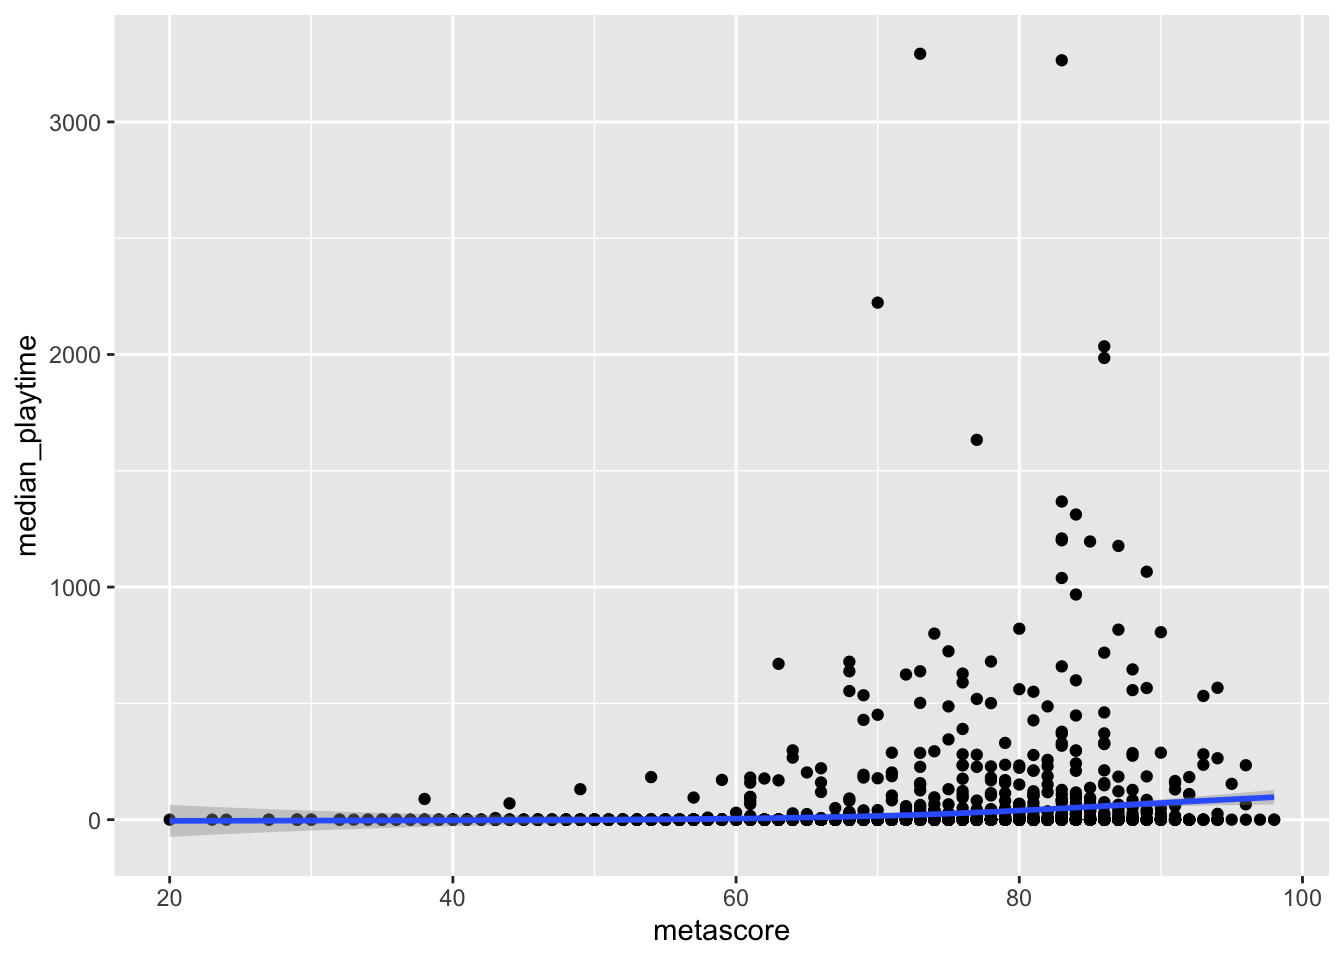
\includegraphics{02-ggplot2_files/figure-latex/unnamed-chunk-34-1.pdf}

\begin{enumerate}
\def\labelenumi{\arabic{enumi}.}
\setcounter{enumi}{4}
\tightlist
\item
  * We can change the y-axis of a histogram to be ``density'' instead of a raw count. This means that each bar shows a \textbf{proportion} of cases instead of a raw count. Google something like ``geom\_histogram with density'' to figure out how to create a y \texttt{aes()} to show density instead of count.
\end{enumerate}

\begin{Shaded}
\begin{Highlighting}[]
\FunctionTok{ggplot}\NormalTok{(}\AttributeTok{data =}\NormalTok{ stat113\_df, }\FunctionTok{aes}\NormalTok{(}\AttributeTok{x =}\NormalTok{ Exercise, }\AttributeTok{y =}\NormalTok{ ..density..)) }\SpecialCharTok{+}
  \FunctionTok{geom\_histogram}\NormalTok{(}\AttributeTok{bins =} \DecValTok{14}\NormalTok{, }\AttributeTok{fill =} \StringTok{"lightpink2"}\NormalTok{, }\AttributeTok{colour =} \StringTok{"black"}\NormalTok{) }\SpecialCharTok{+}
  \FunctionTok{xlab}\NormalTok{(}\StringTok{"Exercise (hours per typical week)"}\NormalTok{)}
\CommentTok{\#\textgreater{} Warning: Removed 7 rows containing non{-}finite values}
\CommentTok{\#\textgreater{} (stat\_bin).}
\end{Highlighting}
\end{Shaded}

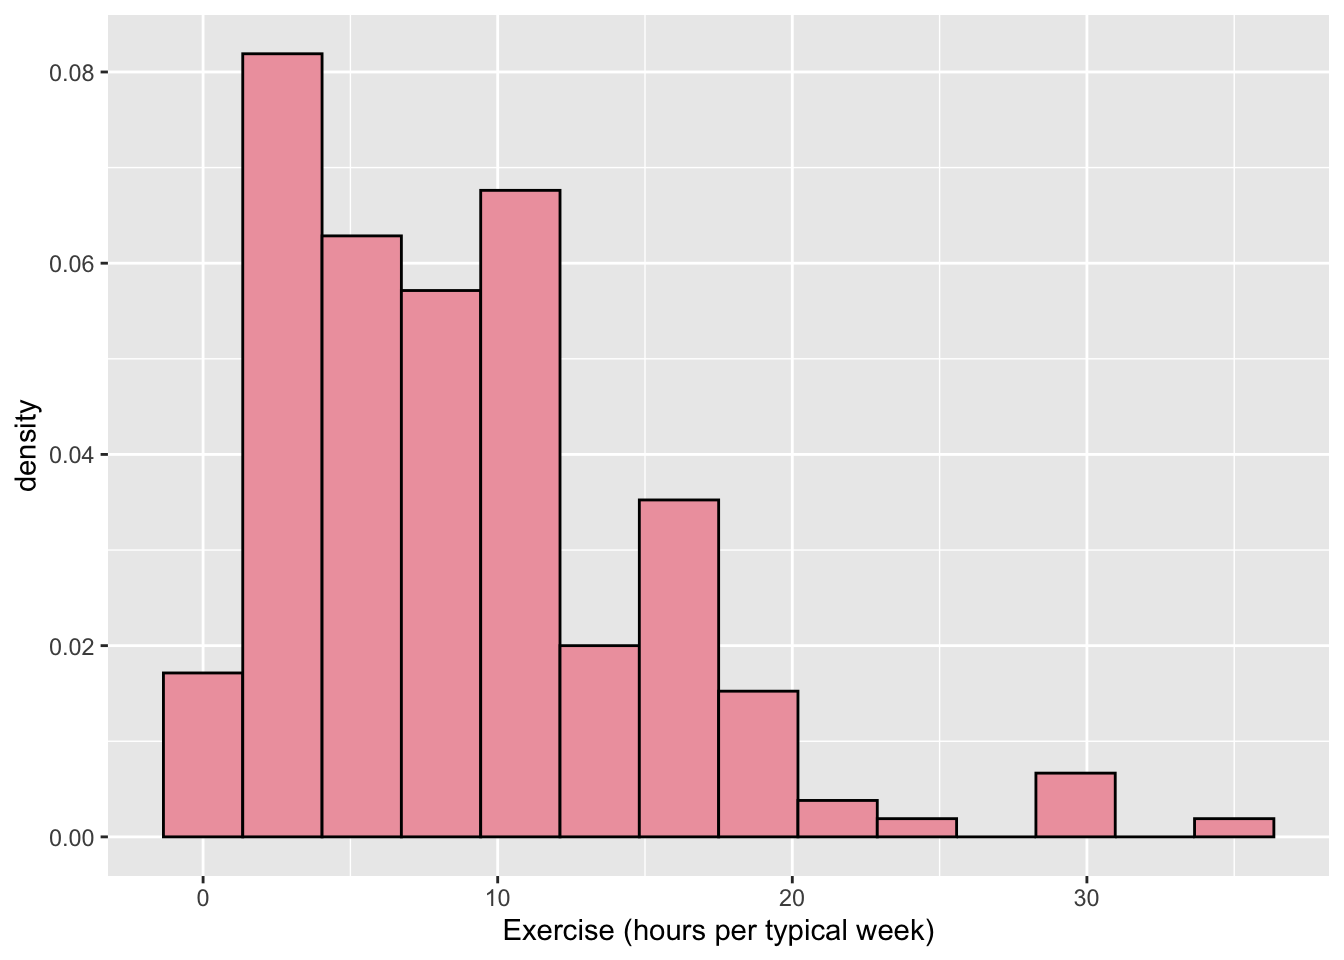
\includegraphics{02-ggplot2_files/figure-latex/unnamed-chunk-35-1.pdf}

\hypertarget{graphing-two-quant.-etc.-s}{%
\subsection{Graphing Two Quant. etc. S}\label{graphing-two-quant.-etc.-s}}

\begin{enumerate}
\def\labelenumi{\arabic{enumi}.}
\setcounter{enumi}{3}
\tightlist
\item
  * Make a scatterplot of \texttt{Hgt} on the y-axis and \texttt{Wgt} on the x-axis, colouring by \texttt{Sport}. Add a smooth fitted curve to your scatterplot. Then, move \texttt{colour\ =\ Sport} from an \texttt{aes()} in the \texttt{ggplot()} function to an \texttt{aes()} in the \texttt{geom\_point()} function. What changes in the plot? Can you give an explanation as to why that change occurs?
\end{enumerate}

\begin{Shaded}
\begin{Highlighting}[]
\FunctionTok{ggplot}\NormalTok{(}\AttributeTok{data =}\NormalTok{ stat113\_df, }\FunctionTok{aes}\NormalTok{(}\AttributeTok{x =}\NormalTok{ Wgt, }\AttributeTok{y =}\NormalTok{ Hgt, }\AttributeTok{colour =}\NormalTok{ Sport)) }\SpecialCharTok{+}
  \FunctionTok{geom\_point}\NormalTok{() }\SpecialCharTok{+}
  \FunctionTok{geom\_smooth}\NormalTok{()}
\end{Highlighting}
\end{Shaded}

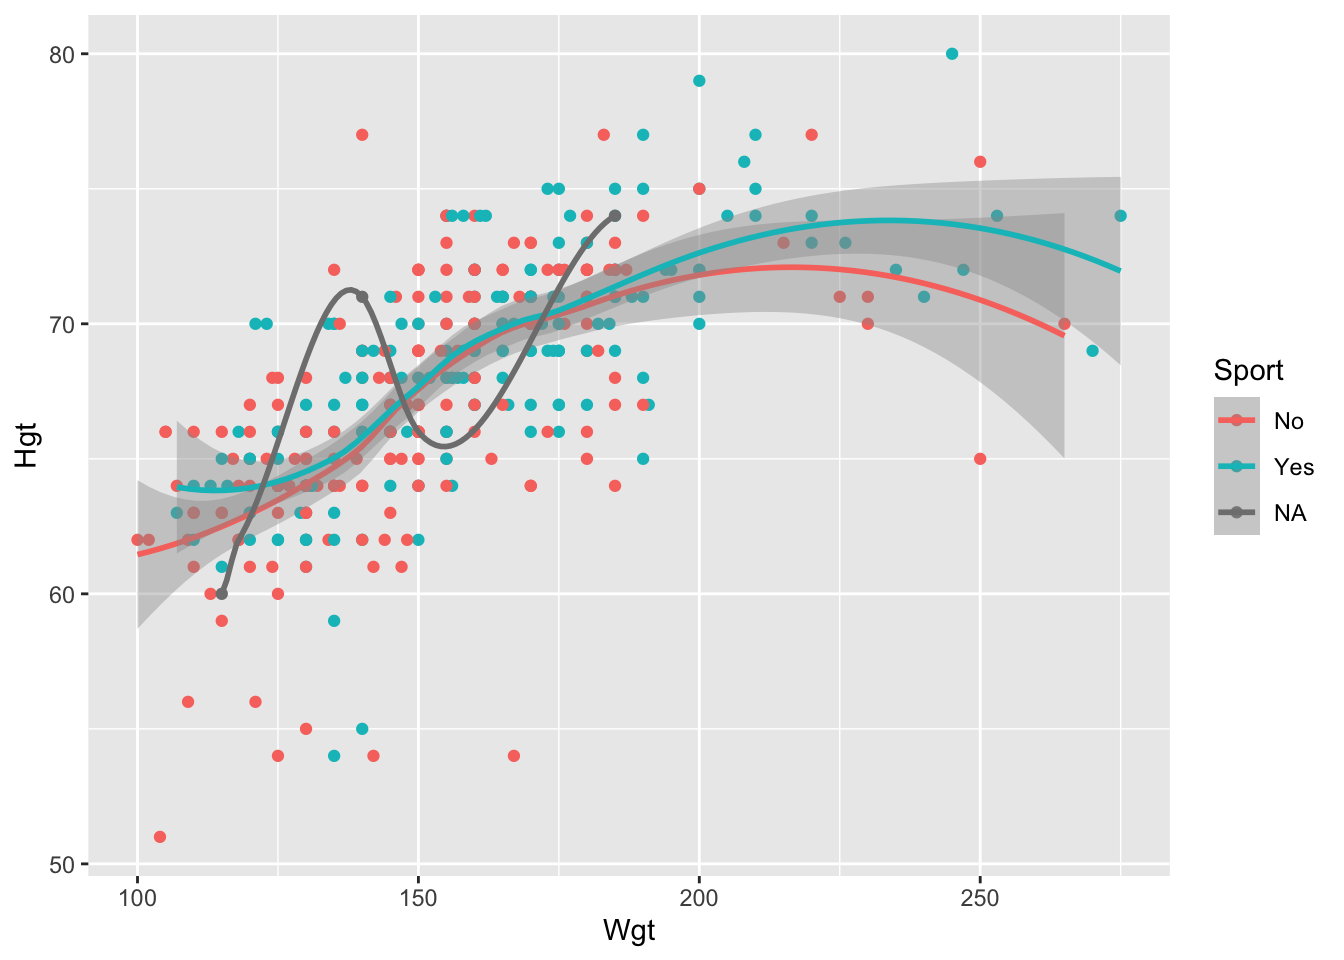
\includegraphics{02-ggplot2_files/figure-latex/unnamed-chunk-36-1.pdf}

\begin{Shaded}
\begin{Highlighting}[]

\FunctionTok{ggplot}\NormalTok{(}\AttributeTok{data =}\NormalTok{ stat113\_df, }\FunctionTok{aes}\NormalTok{(}\AttributeTok{x =}\NormalTok{ Wgt, }\AttributeTok{y =}\NormalTok{ Hgt)) }\SpecialCharTok{+}
  \FunctionTok{geom\_point}\NormalTok{(}\FunctionTok{aes}\NormalTok{(}\AttributeTok{colour =}\NormalTok{ Sport)) }\SpecialCharTok{+}
  \FunctionTok{geom\_smooth}\NormalTok{()}
\end{Highlighting}
\end{Shaded}

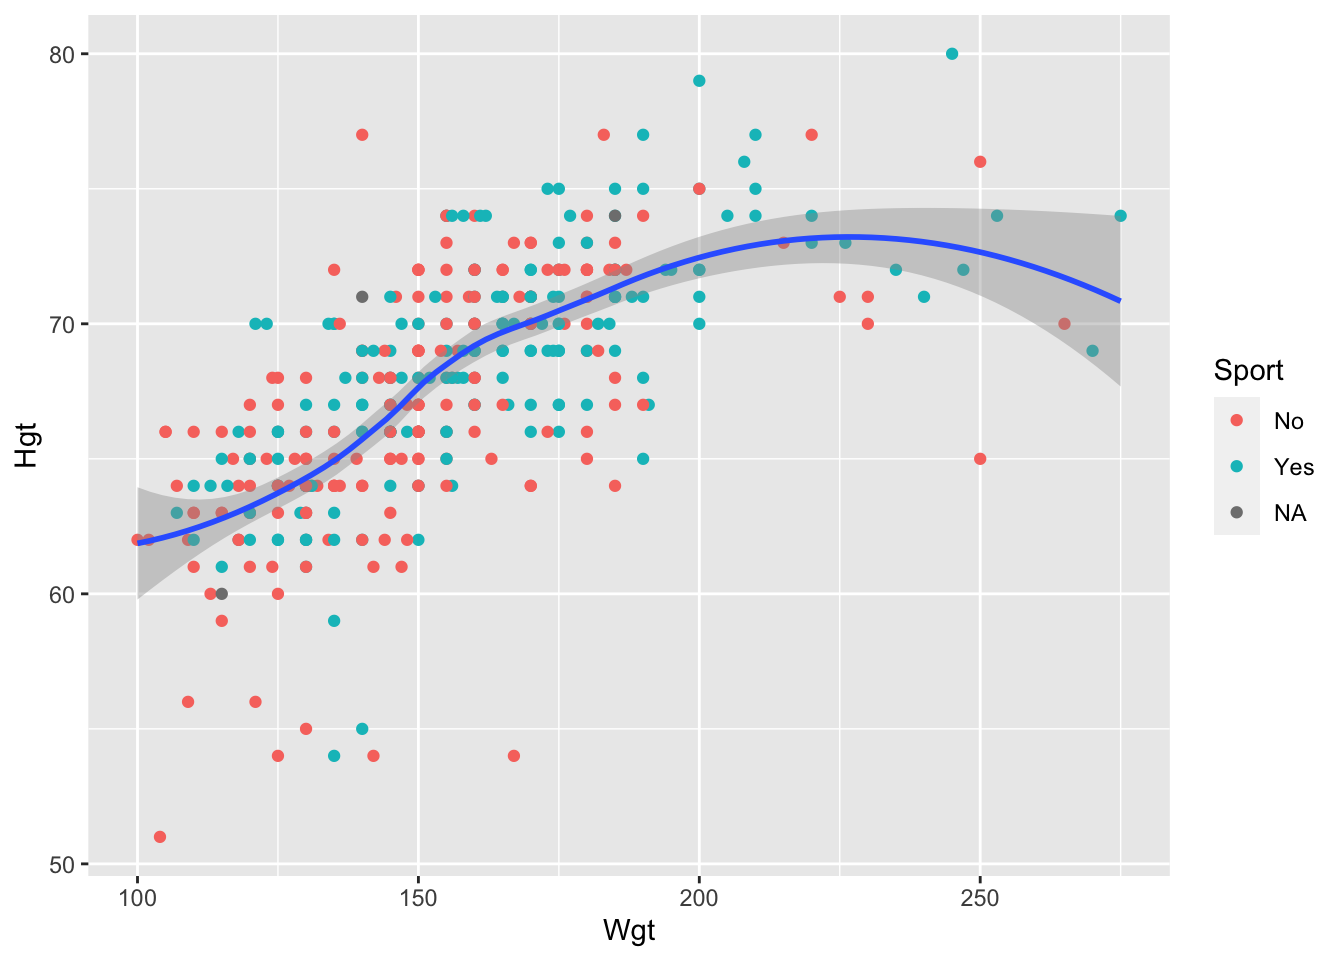
\includegraphics{02-ggplot2_files/figure-latex/unnamed-chunk-36-2.pdf}

The points are now coloured by \texttt{Sport} but there is only one smooth fitted line. This makes sense because \texttt{geom\_point()} now has the two global aesthetics x and y, as well as the colour aesthetic. \texttt{geom\_smooth()} no longer has the colour aesthetic but still inherits the two global aesthetics, x and y.

\begin{enumerate}
\def\labelenumi{\arabic{enumi}.}
\setcounter{enumi}{4}
\tightlist
\item
  * Faceting can be used for other types of plots too! Make a pair of faceted histograms for a quantitative variable of your choosing that are faceted by a categorical variable of your choosing.
\end{enumerate}

Answers will vary:

\begin{Shaded}
\begin{Highlighting}[]
\FunctionTok{ggplot}\NormalTok{(}\AttributeTok{data =}\NormalTok{ stat113\_df, }\FunctionTok{aes}\NormalTok{(}\AttributeTok{x =}\NormalTok{ GPA)) }\SpecialCharTok{+} 
  \FunctionTok{geom\_histogram}\NormalTok{(}\AttributeTok{bins =} \DecValTok{15}\NormalTok{) }\SpecialCharTok{+}
  \FunctionTok{facet\_wrap}\NormalTok{( }\SpecialCharTok{\textasciitilde{}}\NormalTok{ Sport)}
\end{Highlighting}
\end{Shaded}

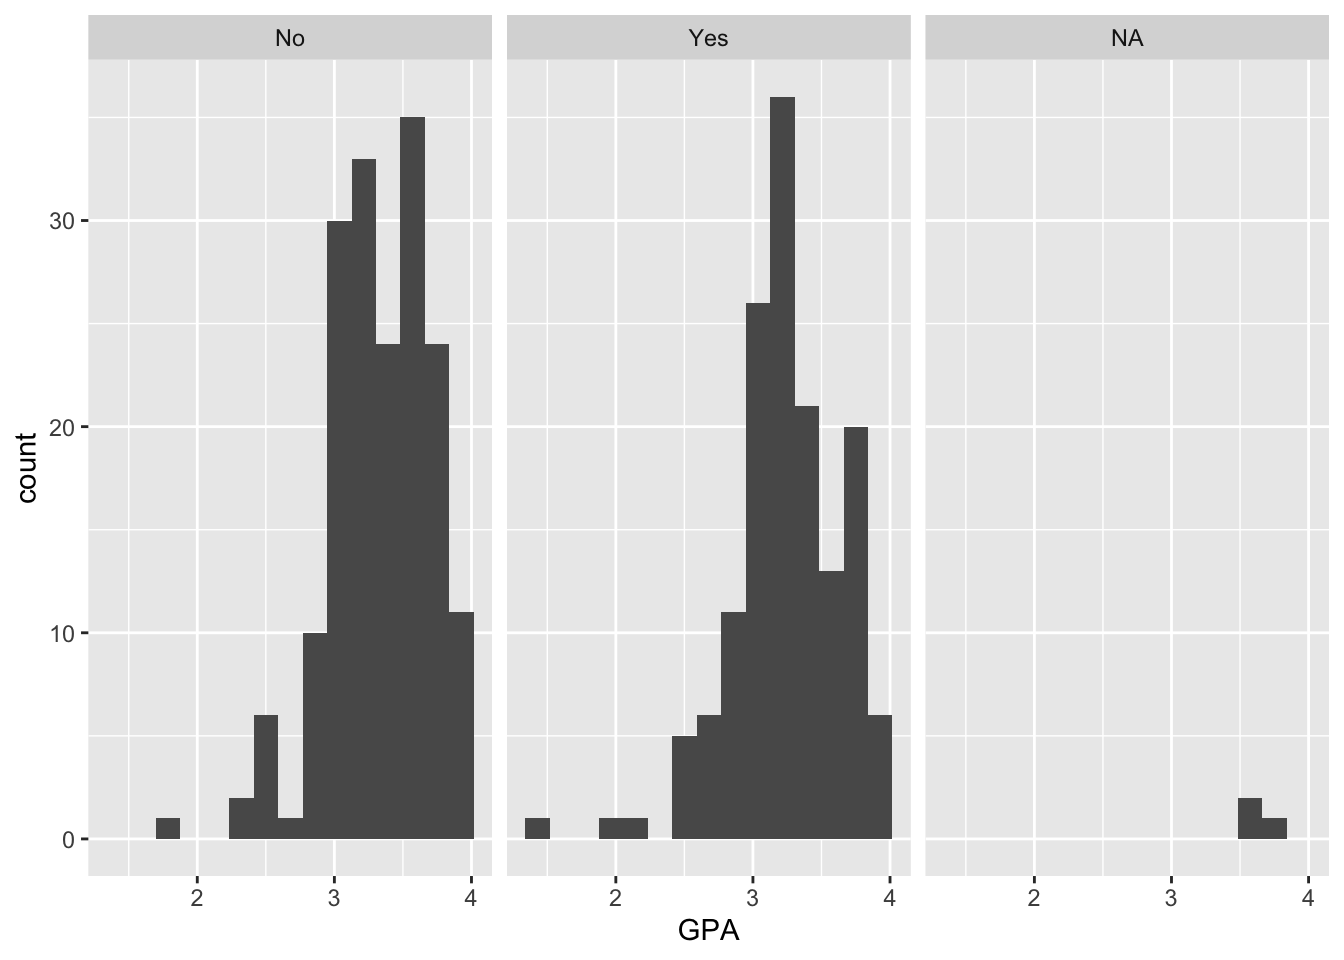
\includegraphics{02-ggplot2_files/figure-latex/unnamed-chunk-37-1.pdf}

\hypertarget{boxplots-stacked-etc.-s}{%
\subsection{Boxplots, Stacked, etc. S}\label{boxplots-stacked-etc.-s}}

\begin{enumerate}
\def\labelenumi{\arabic{enumi}.}
\tightlist
\item
  * Change the colour of the inside of the boxplots in the Exercise vs.~Award graph to be \texttt{"blue"}. Do you think you'll use \texttt{colour\ =\ "blue"} or \texttt{fill\ =\ "blue"}?
\end{enumerate}

\begin{Shaded}
\begin{Highlighting}[]
\FunctionTok{ggplot}\NormalTok{(}\AttributeTok{data =}\NormalTok{ stat113\_df, }\FunctionTok{aes}\NormalTok{(}\AttributeTok{x =}\NormalTok{ Award, }\AttributeTok{y =}\NormalTok{ Exercise)) }\SpecialCharTok{+}
  \FunctionTok{geom\_boxplot}\NormalTok{(}\AttributeTok{fill =} \StringTok{"blue"}\NormalTok{)}
\CommentTok{\#\textgreater{} Warning: Removed 7 rows containing non{-}finite values}
\CommentTok{\#\textgreater{} (stat\_boxplot).}
\end{Highlighting}
\end{Shaded}

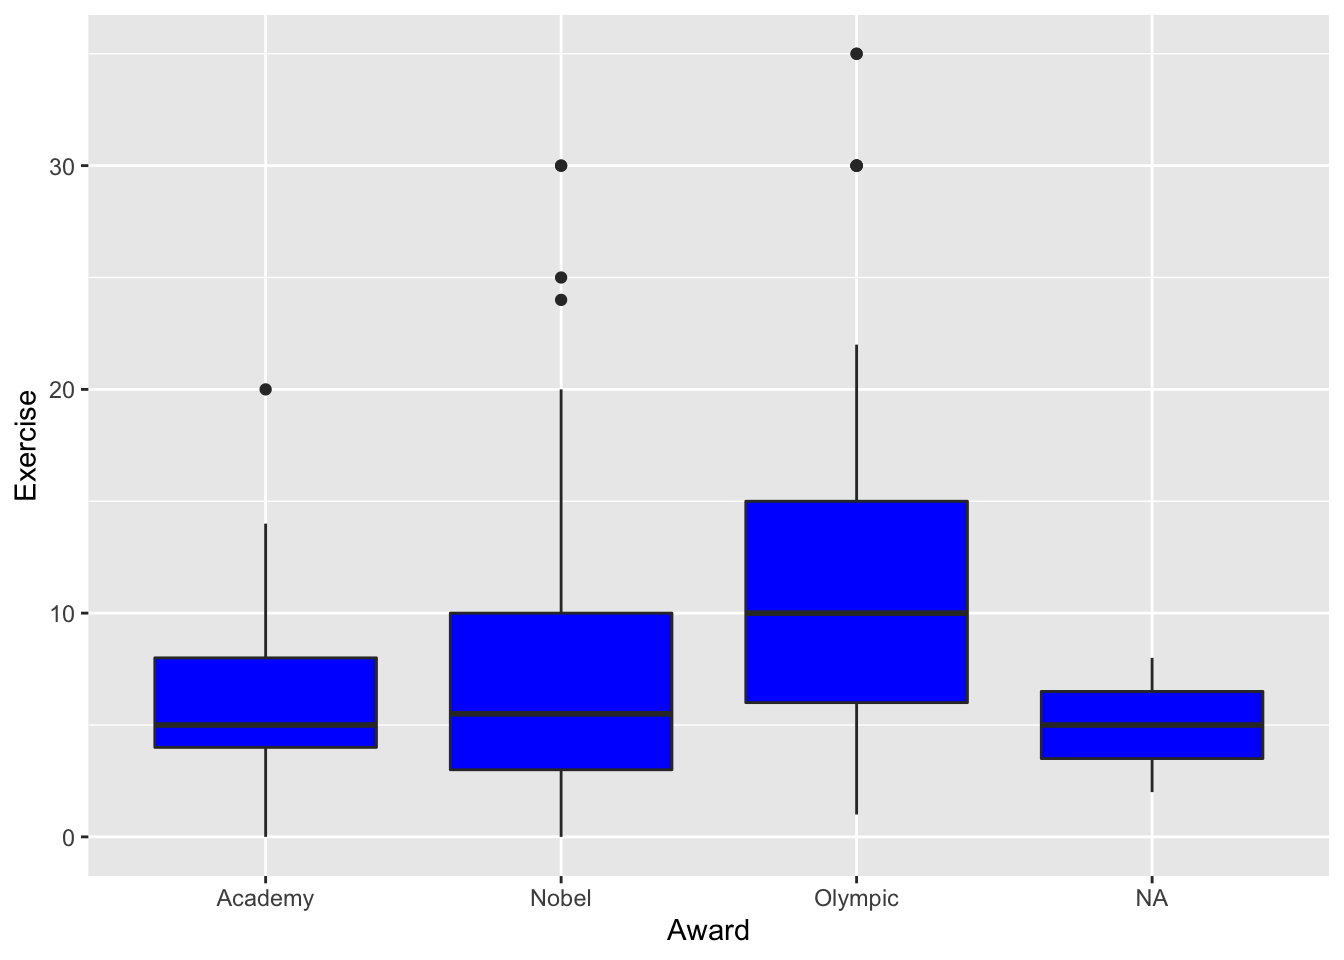
\includegraphics{02-ggplot2_files/figure-latex/unnamed-chunk-38-1.pdf}

\texttt{fill} because it's the inside of the boxplots that we want to modify. \texttt{colour} will modify the outline colour.

\begin{enumerate}
\def\labelenumi{\arabic{enumi}.}
\setcounter{enumi}{1}
\tightlist
\item
  * Create a side-by-side boxplot that compares the \texttt{GPA}s of students who prefer different \texttt{Award}s. Then change the fill of the boxplot to be a colour of your choice. What do you notice in the plot?
\end{enumerate}

\begin{Shaded}
\begin{Highlighting}[]
\FunctionTok{ggplot}\NormalTok{(}\AttributeTok{data =}\NormalTok{ stat113\_df, }\FunctionTok{aes}\NormalTok{(}\AttributeTok{x =}\NormalTok{ Award, }\AttributeTok{y =}\NormalTok{ GPA)) }\SpecialCharTok{+}
  \FunctionTok{geom\_boxplot}\NormalTok{(}\AttributeTok{fill =} \StringTok{"lightpink1"}\NormalTok{)}
\CommentTok{\#\textgreater{} Warning: Removed 70 rows containing non{-}finite values}
\CommentTok{\#\textgreater{} (stat\_boxplot).}
\end{Highlighting}
\end{Shaded}

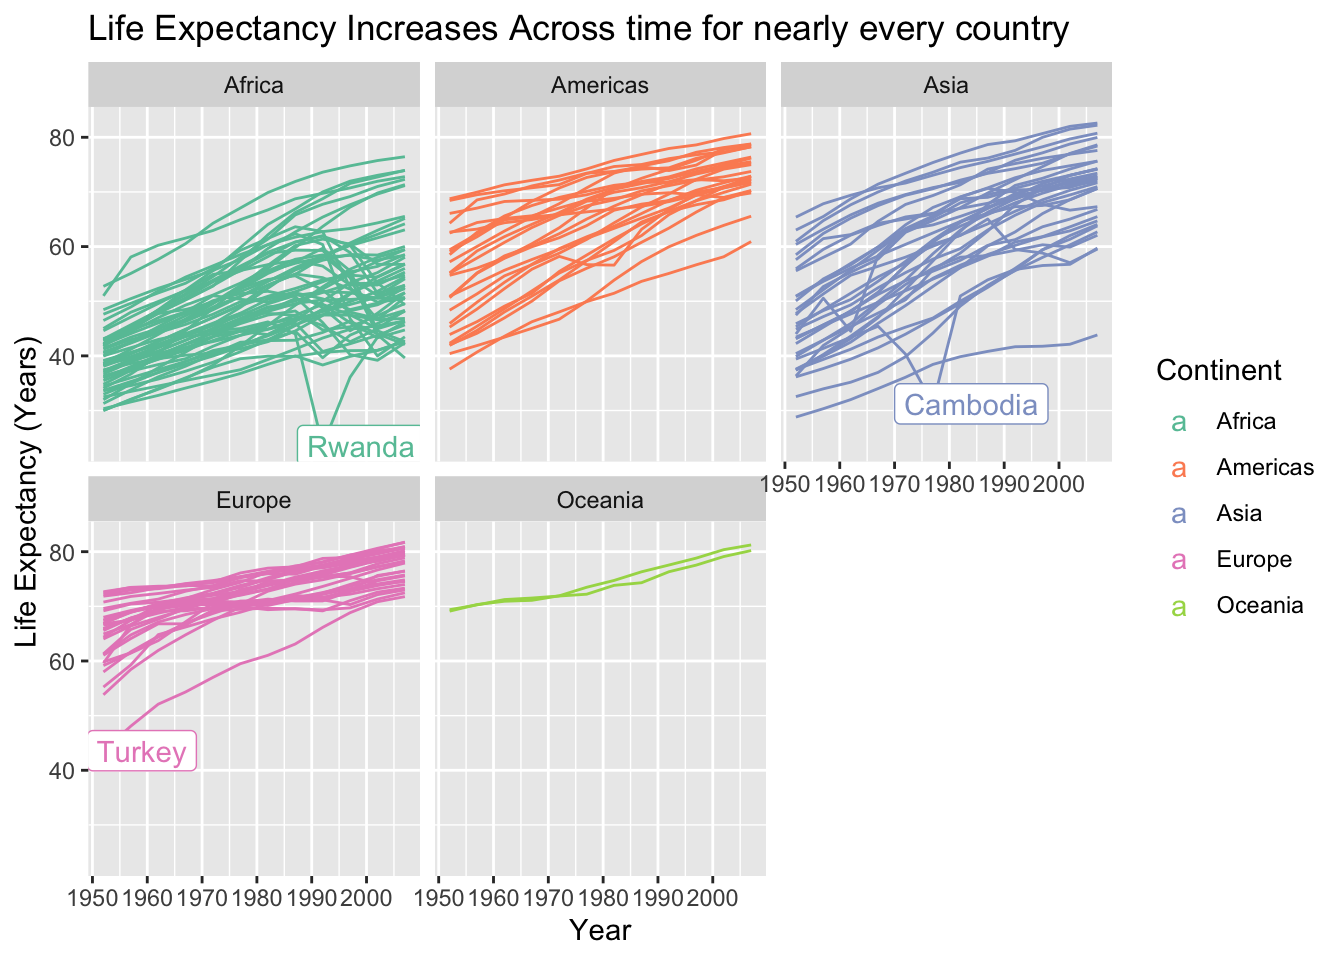
\includegraphics{02-ggplot2_files/figure-latex/unnamed-chunk-39-1.pdf}

There are a few outlier students, but the three groups overall seem to have similar GPAs.

\begin{enumerate}
\def\labelenumi{\arabic{enumi}.}
\setcounter{enumi}{2}
\tightlist
\item
  * When making the previous plot, \texttt{R} gives us a warning message that it ``Removed 70 rows containing non-finite values''. This is \texttt{R}'s robotic way of telling us that 70 \texttt{GPA} values are missing in the data set. Use what you know about how the data was collected (Fall and Spring semeseter of the 2018-2019 school-year) to guess why these are missing.
\end{enumerate}

STAT 113 has first-year students: first-years taking the course in the fall would not have a GPA to report. Additionally, another reason might be that a student chose not to report his or her GPA.

\begin{enumerate}
\def\labelenumi{\arabic{enumi}.}
\setcounter{enumi}{3}
\tightlist
\item
  * Make a stacked bar plot for two variables of your choosing in the STAT 113 data set. Comment on something that you notice in the plot.
\end{enumerate}

Answers will vary.

\begin{Shaded}
\begin{Highlighting}[]
\FunctionTok{ggplot}\NormalTok{(}\AttributeTok{data =}\NormalTok{ stat113\_df, }\FunctionTok{aes}\NormalTok{(}\AttributeTok{x =}\NormalTok{ Sport, }\AttributeTok{fill =}\NormalTok{ Award)) }\SpecialCharTok{+}
  \FunctionTok{geom\_bar}\NormalTok{(}\AttributeTok{position =} \StringTok{"fill"}\NormalTok{)}
\end{Highlighting}
\end{Shaded}

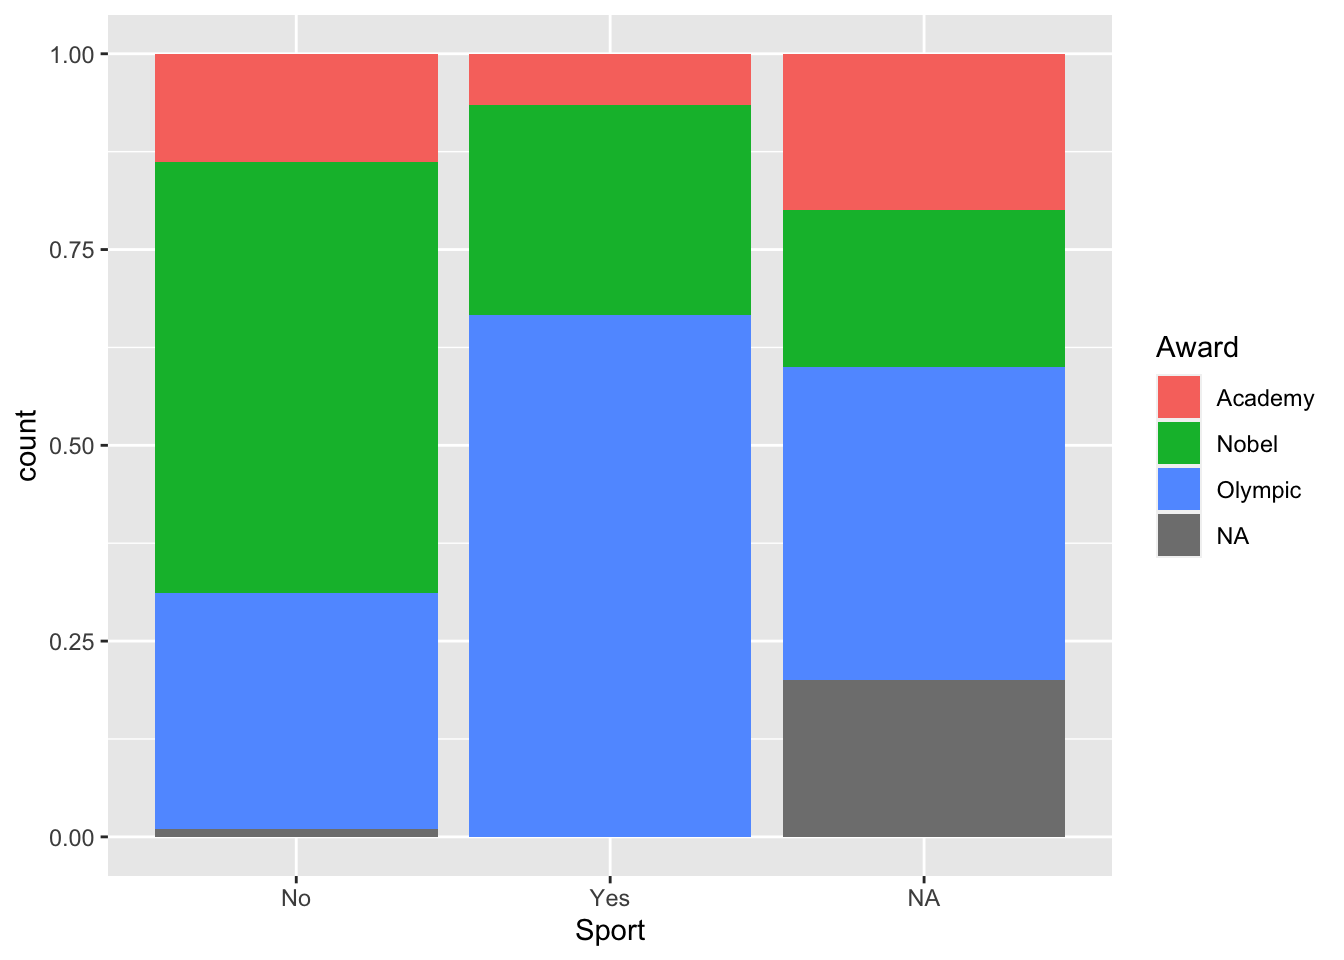
\includegraphics{02-ggplot2_files/figure-latex/unnamed-chunk-40-1.pdf}

As we might expect, it does seem like a higher proportion of students who play a sport would prefer to win an Olympic medal, compared with students who do not play a sport.

\hypertarget{chapexercise-2-S}{%
\subsection{Chapter Exercises S}\label{chapexercise-2-S}}

\begin{enumerate}
\def\labelenumi{\arabic{enumi}.}
\tightlist
\item
  * The default of \texttt{geom\_smooth()} is to use LOESS (locally estimated scatterplot smoothing). Read about LOESS here: here. Write one or two sentences explaining what LOESS does.
\end{enumerate}

Loess uses a bunch of local regressions to predict the y-variable at each point, giving more weight to observations near the point of interest on the x-axis. Once this is done for every point, the predictions are connected with a smooth curve.

\begin{enumerate}
\def\labelenumi{\arabic{enumi}.}
\setcounter{enumi}{1}
\tightlist
\item
  * Thus far, we have only faceted by a single variable. Use Google to figure out how to facet by two variables to make a plot that shows the relationship between GPA (y-axis) and Exercise (x-axis) with four facets: one for male students who play a sport, one for female students who play a sport, one for male students who do not play a sport, and one for female students who do not play a sport.
\end{enumerate}

\begin{Shaded}
\begin{Highlighting}[]
\FunctionTok{ggplot}\NormalTok{(}\AttributeTok{data =}\NormalTok{ stat113\_df }\SpecialCharTok{\%\textgreater{}\%} \FunctionTok{filter}\NormalTok{(}\SpecialCharTok{!}\FunctionTok{is.na}\NormalTok{(Sport) }\SpecialCharTok{\&} \SpecialCharTok{!}\FunctionTok{is.na}\NormalTok{(Sex)),}
  \FunctionTok{aes}\NormalTok{(}\AttributeTok{x =}\NormalTok{ Exercise, }\AttributeTok{y =}\NormalTok{ GPA)) }\SpecialCharTok{+} 
  \FunctionTok{geom\_point}\NormalTok{() }\SpecialCharTok{+} \FunctionTok{geom\_smooth}\NormalTok{() }\SpecialCharTok{+}
  \FunctionTok{facet\_grid}\NormalTok{(Sex }\SpecialCharTok{\textasciitilde{}}\NormalTok{ Sport)}
\CommentTok{\#\textgreater{} \textasciigrave{}geom\_smooth()\textasciigrave{} using method = \textquotesingle{}loess\textquotesingle{} and formula \textquotesingle{}y \textasciitilde{} x\textquotesingle{}}
\CommentTok{\#\textgreater{} Warning: Removed 71 rows containing non{-}finite values}
\CommentTok{\#\textgreater{} (stat\_smooth).}
\CommentTok{\#\textgreater{} Warning: Removed 71 rows containing missing values}
\CommentTok{\#\textgreater{} (geom\_point).}
\end{Highlighting}
\end{Shaded}

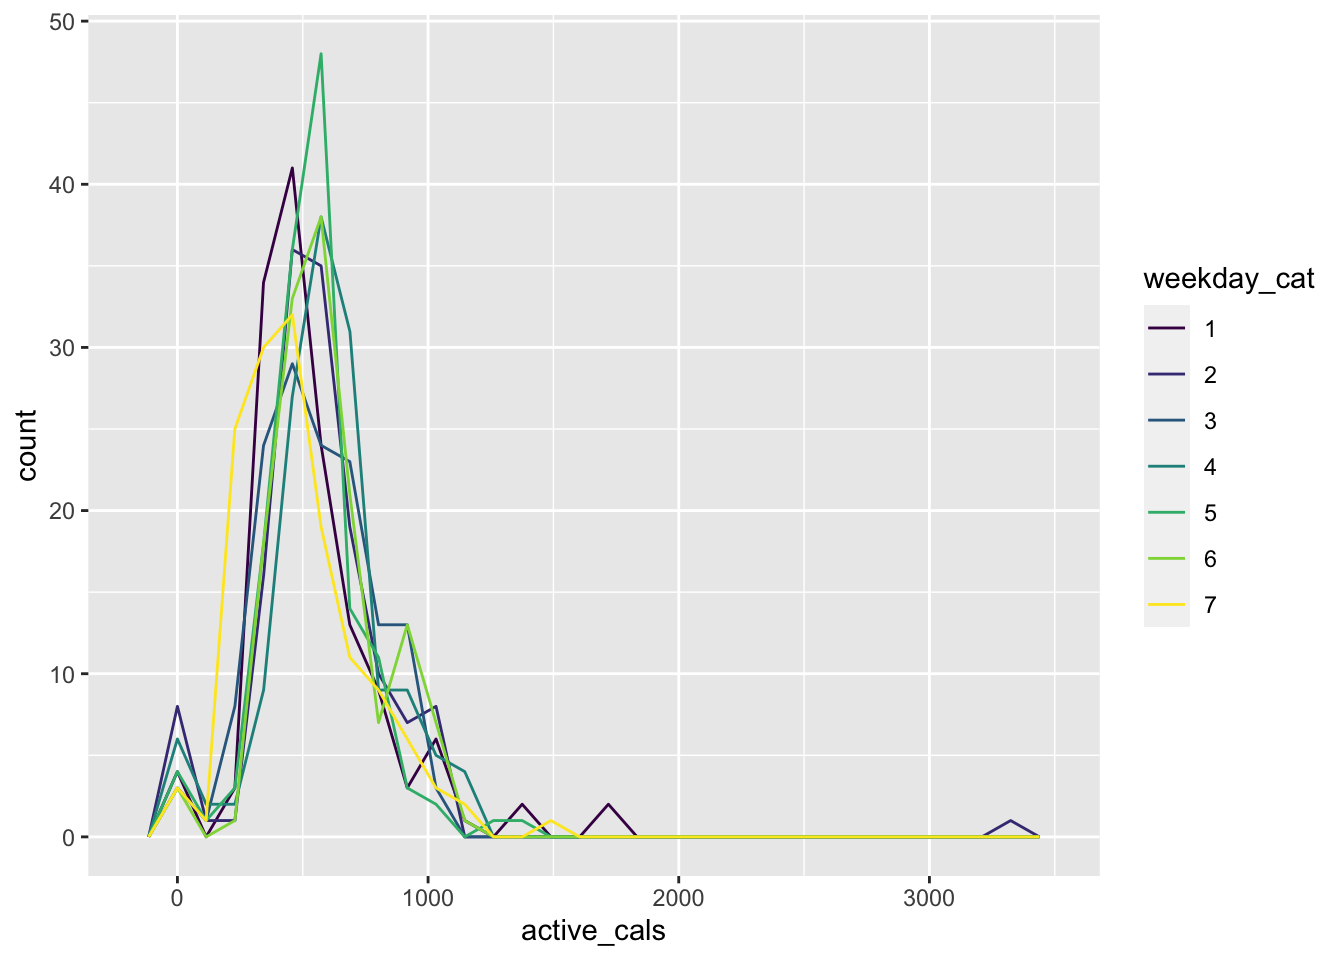
\includegraphics{02-ggplot2_files/figure-latex/unnamed-chunk-41-1.pdf}

\begin{enumerate}
\def\labelenumi{\arabic{enumi}.}
\setcounter{enumi}{2}
\tightlist
\item
  * In Intro-Stat, boxplots are typically introduced using the \texttt{*} symbol to identify outliers. Using a combination of the help \texttt{?geom\_boxplot} and Googling ``R point shapes'', figure out how to modify your side-by-side boxplots so that the outliers are shown using \texttt{*}, not the default dots.
\end{enumerate}

Then, using Google, figure out how to add the mean to each boxplot as a ``darkgreen'' diamond-shaped symbol with \texttt{stat\_summary()}.

\begin{Shaded}
\begin{Highlighting}[]
\FunctionTok{ggplot}\NormalTok{(}\AttributeTok{data =}\NormalTok{ stat113\_df, }\FunctionTok{aes}\NormalTok{(}\AttributeTok{x =}\NormalTok{ Sex, }\AttributeTok{y =}\NormalTok{ GPA)) }\SpecialCharTok{+}
  \FunctionTok{geom\_boxplot}\NormalTok{(}\AttributeTok{fill =} \StringTok{"lightpink1"}\NormalTok{, }\AttributeTok{outlier.shape =} \DecValTok{8}\NormalTok{) }\SpecialCharTok{+}
  \FunctionTok{stat\_summary}\NormalTok{(}\AttributeTok{fun =}\NormalTok{ mean, }\AttributeTok{shape =} \DecValTok{18}\NormalTok{, }\AttributeTok{colour =} \StringTok{"darkgreen"}\NormalTok{)}
\CommentTok{\#\textgreater{} Warning: Removed 70 rows containing non{-}finite values}
\CommentTok{\#\textgreater{} (stat\_boxplot).}
\CommentTok{\#\textgreater{} Warning: Removed 70 rows containing non{-}finite values}
\CommentTok{\#\textgreater{} (stat\_summary).}
\CommentTok{\#\textgreater{} Warning: Removed 3 rows containing missing values}
\CommentTok{\#\textgreater{} (geom\_segment).}
\end{Highlighting}
\end{Shaded}

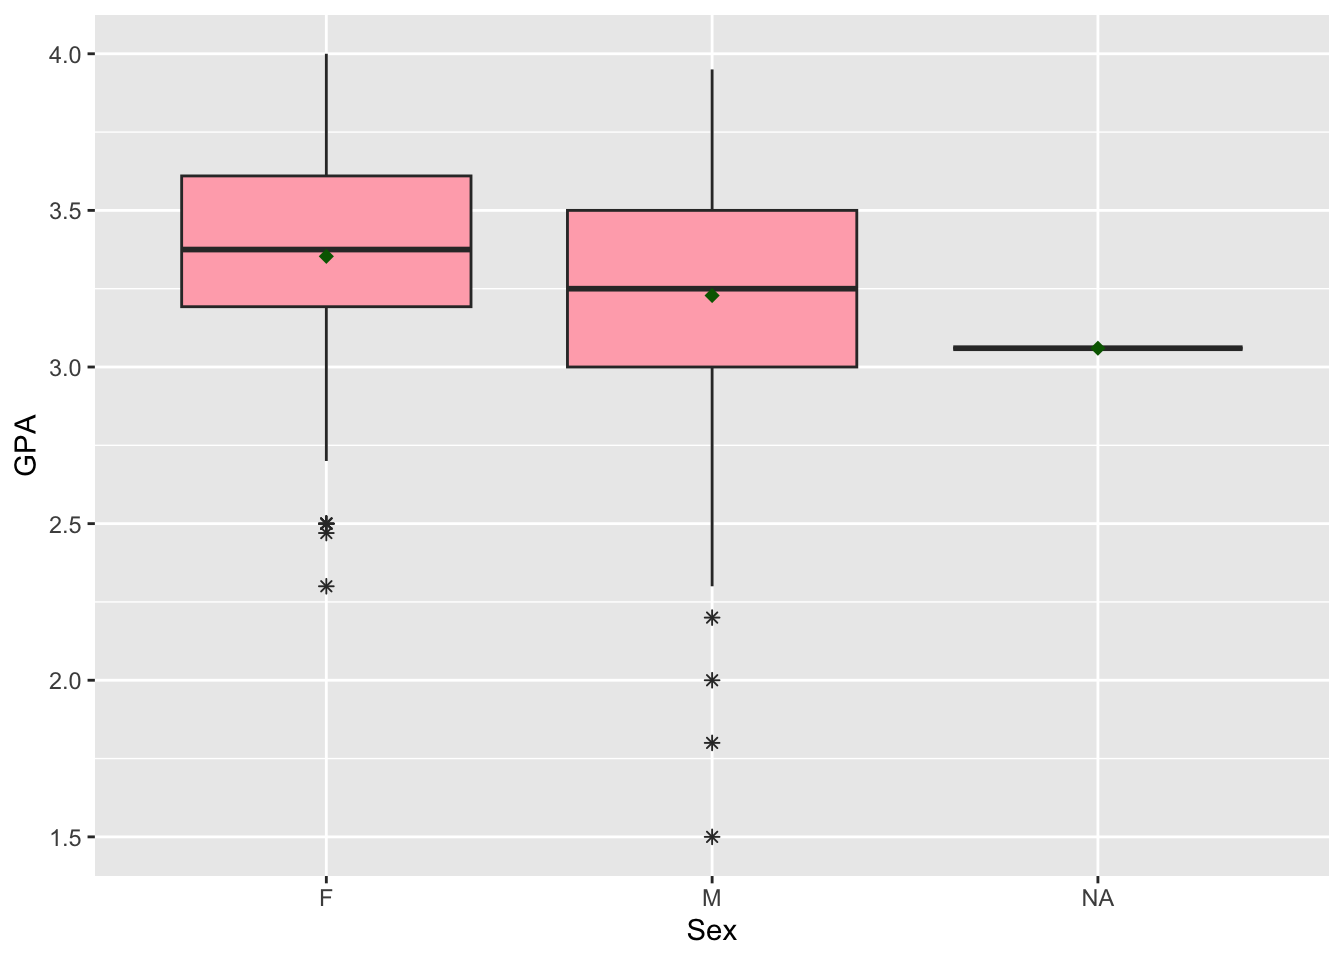
\includegraphics{02-ggplot2_files/figure-latex/unnamed-chunk-42-1.pdf}

\hypertarget{rcode-2}{%
\section{\texorpdfstring{Non-Exercise \texttt{R} Code}{Non-Exercise R Code}}\label{rcode-2}}

\begin{Shaded}
\begin{Highlighting}[]
\FunctionTok{library}\NormalTok{(tidyverse)}
\NormalTok{pres\_df }\OtherTok{\textless{}{-}} \FunctionTok{read\_table}\NormalTok{(}\StringTok{"data/PRES2000.txt"}\NormalTok{) }
\DocumentationTok{\#\# don\textquotesingle{}t worry about the \textasciigrave{}read\_table\textasciigrave{} function....yet}
\FunctionTok{head}\NormalTok{(pres\_df)}
\FunctionTok{ggplot}\NormalTok{(}\AttributeTok{data =}\NormalTok{ pres\_df, }\AttributeTok{mapping =} \FunctionTok{aes}\NormalTok{(}\AttributeTok{x =}\NormalTok{ Gore)) }\SpecialCharTok{+}
  \FunctionTok{geom\_histogram}\NormalTok{(}\AttributeTok{colour =} \StringTok{"black"}\NormalTok{, }\AttributeTok{fill =} \StringTok{"white"}\NormalTok{) }\SpecialCharTok{+}
  \FunctionTok{xlab}\NormalTok{(}\StringTok{"Votes for Gore in Florida"}\NormalTok{)}
\FunctionTok{ggplot}\NormalTok{(}\AttributeTok{data =}\NormalTok{ pres\_df, }\AttributeTok{mapping =} \FunctionTok{aes}\NormalTok{(}\AttributeTok{x =}\NormalTok{ Gore)) }\SpecialCharTok{+}
  \FunctionTok{geom\_freqpoly}\NormalTok{(}\AttributeTok{colour =} \StringTok{"black"}\NormalTok{) }\SpecialCharTok{+}
  \FunctionTok{xlab}\NormalTok{(}\StringTok{"Votes for Gore in Florida"}\NormalTok{) }
\FunctionTok{ggplot}\NormalTok{(}\AttributeTok{data =}\NormalTok{ pres\_df, }\AttributeTok{mapping =} \FunctionTok{aes}\NormalTok{(}\AttributeTok{x =}\NormalTok{ Gore)) }\SpecialCharTok{+}
  \FunctionTok{geom\_freqpoly}\NormalTok{(}\AttributeTok{colour =} \StringTok{"black"}\NormalTok{) }\SpecialCharTok{+}
  \FunctionTok{xlab}\NormalTok{(}\StringTok{"Votes for Gore in Florida"}\NormalTok{) }\SpecialCharTok{+}
  \FunctionTok{geom\_histogram}\NormalTok{() }
\NormalTok{pres\_cat }\OtherTok{\textless{}{-}}\NormalTok{ pres\_df }\SpecialCharTok{\%\textgreater{}\%} \FunctionTok{mutate}\NormalTok{(}\AttributeTok{winner =} \FunctionTok{if\_else}\NormalTok{(Gore }\SpecialCharTok{\textgreater{}}\NormalTok{ Bush,}
                                                \AttributeTok{true =} \StringTok{"Gore"}\NormalTok{,}
                                                \AttributeTok{false =} \StringTok{"Bush"}\NormalTok{))}
\NormalTok{pres\_cat}
\FunctionTok{ggplot}\NormalTok{(}\AttributeTok{data =}\NormalTok{ pres\_cat, }\FunctionTok{aes}\NormalTok{(}\AttributeTok{x =}\NormalTok{ winner)) }\SpecialCharTok{+}
  \FunctionTok{geom\_bar}\NormalTok{()}
\NormalTok{pres\_cat2 }\OtherTok{\textless{}{-}}\NormalTok{ pres\_cat }\SpecialCharTok{\%\textgreater{}\%} \FunctionTok{group\_by}\NormalTok{(winner) }\SpecialCharTok{\%\textgreater{}\%}
  \FunctionTok{summarise}\NormalTok{(}\AttributeTok{nwins =} \FunctionTok{n}\NormalTok{())}
\NormalTok{pres\_cat2}
\FunctionTok{ggplot}\NormalTok{(pres\_cat2, }\FunctionTok{aes}\NormalTok{(}\AttributeTok{x =}\NormalTok{ winner)) }\SpecialCharTok{+}
  \FunctionTok{geom\_bar}\NormalTok{()}
\FunctionTok{ggplot}\NormalTok{(pres\_cat2, }\FunctionTok{aes}\NormalTok{(}\AttributeTok{x =}\NormalTok{ winner, }\AttributeTok{y =}\NormalTok{ nwins)) }\SpecialCharTok{+}
  \FunctionTok{geom\_col}\NormalTok{()}
\FunctionTok{ggplot}\NormalTok{(}\AttributeTok{data =}\NormalTok{ pres\_df, }\AttributeTok{mapping =} \FunctionTok{aes}\NormalTok{(}\AttributeTok{x =}\NormalTok{ Gore, }\AttributeTok{y =}\NormalTok{ Bush)) }\SpecialCharTok{+}
  \FunctionTok{geom\_point}\NormalTok{()}
\FunctionTok{library}\NormalTok{(tidyverse)}
\NormalTok{fitness\_full }\OtherTok{\textless{}{-}} \FunctionTok{read\_csv}\NormalTok{(}\StringTok{"data/higham\_fitness\_clean.csv"}\NormalTok{) }\SpecialCharTok{\%\textgreater{}\%} \FunctionTok{mutate}\NormalTok{(}\AttributeTok{weekend\_ind =} \FunctionTok{case\_when}\NormalTok{(weekday }\SpecialCharTok{==} \StringTok{"Sat"} \SpecialCharTok{|}\NormalTok{ weekday }\SpecialCharTok{==} \StringTok{"Sun"} \SpecialCharTok{\textasciitilde{}} \StringTok{"weekend"}\NormalTok{,}
  \ConstantTok{TRUE} \SpecialCharTok{\textasciitilde{}} \StringTok{"weekday"}\NormalTok{))}
\FunctionTok{ggplot}\NormalTok{(}\AttributeTok{data =}\NormalTok{ fitness\_full, }\FunctionTok{aes}\NormalTok{(}\AttributeTok{x =}\NormalTok{ distance, }\AttributeTok{y =}\NormalTok{ active\_cals)) }\SpecialCharTok{+}
  \FunctionTok{geom\_point}\NormalTok{()}
\DocumentationTok{\#\# drop observations that have active calories \textless{} 50. }
\DocumentationTok{\#\# assuming that these are data errors or }
\DocumentationTok{\#\# days where the Apple Watch wasn\textquotesingle{}t worn.}
\NormalTok{fitness }\OtherTok{\textless{}{-}}\NormalTok{ fitness\_full }\SpecialCharTok{\%\textgreater{}\%}
  \FunctionTok{filter}\NormalTok{(active\_cals }\SpecialCharTok{\textgreater{}} \DecValTok{50}\NormalTok{)}
\FunctionTok{ggplot}\NormalTok{(}\AttributeTok{data =}\NormalTok{ fitness) }\SpecialCharTok{+}
  \FunctionTok{geom\_point}\NormalTok{(}\FunctionTok{aes}\NormalTok{(}\AttributeTok{x =}\NormalTok{ distance, }\AttributeTok{y =}\NormalTok{ active\_cals))}
\FunctionTok{ggplot}\NormalTok{(}\AttributeTok{data =}\NormalTok{ fitness) }\SpecialCharTok{+}
  \FunctionTok{geom\_point}\NormalTok{(}\FunctionTok{aes}\NormalTok{(}\AttributeTok{x =}\NormalTok{ Start, }\AttributeTok{y =}\NormalTok{ active\_cals, }\AttributeTok{colour =}\NormalTok{ weekend\_ind))}
\FunctionTok{ggplot}\NormalTok{(}\AttributeTok{data =}\NormalTok{ fitness) }\SpecialCharTok{+}
  \FunctionTok{geom\_point}\NormalTok{(}\FunctionTok{aes}\NormalTok{(}\AttributeTok{x =}\NormalTok{ Start, }\AttributeTok{y =}\NormalTok{ active\_cals, }\AttributeTok{shape =}\NormalTok{ weekend\_ind))}
\FunctionTok{ggplot}\NormalTok{(}\AttributeTok{data =}\NormalTok{ fitness) }\SpecialCharTok{+}
  \FunctionTok{geom\_point}\NormalTok{(}\FunctionTok{aes}\NormalTok{(}\AttributeTok{x =}\NormalTok{ Start, }\AttributeTok{y =}\NormalTok{ active\_cals, }\AttributeTok{size =}\NormalTok{ flights))}
\FunctionTok{ggplot}\NormalTok{(}\AttributeTok{data =}\NormalTok{ fitness) }\SpecialCharTok{+}
  \FunctionTok{geom\_point}\NormalTok{(}\FunctionTok{aes}\NormalTok{(}\AttributeTok{x =}\NormalTok{ Start, }\AttributeTok{y =}\NormalTok{ active\_cals, }\AttributeTok{colour =} \StringTok{"purple"}\NormalTok{))}
\FunctionTok{ggplot}\NormalTok{(}\AttributeTok{data =}\NormalTok{ fitness) }\SpecialCharTok{+}
  \FunctionTok{geom\_point}\NormalTok{(}\FunctionTok{aes}\NormalTok{(}\AttributeTok{x =}\NormalTok{ Start, }\AttributeTok{y =}\NormalTok{ active\_cals), }\AttributeTok{size =} \FloatTok{1.5}\NormalTok{, }\AttributeTok{shape =} \DecValTok{19}\NormalTok{)}
\FunctionTok{ggplot}\NormalTok{(}\AttributeTok{data =}\NormalTok{ fitness, }\FunctionTok{aes}\NormalTok{(}\AttributeTok{x =}\NormalTok{ Start, }\AttributeTok{y =}\NormalTok{ active\_cals)) }\SpecialCharTok{+}
  \FunctionTok{geom\_point}\NormalTok{() }\SpecialCharTok{+}
  \FunctionTok{geom\_smooth}\NormalTok{()}
\FunctionTok{ggplot}\NormalTok{(}\AttributeTok{data =}\NormalTok{ fitness, }\FunctionTok{aes}\NormalTok{(}\AttributeTok{x =}\NormalTok{ Start, }\AttributeTok{y =}\NormalTok{ active\_cals)) }\SpecialCharTok{+}
  \FunctionTok{geom\_point}\NormalTok{() }\SpecialCharTok{+}
  \FunctionTok{geom\_smooth}\NormalTok{(}\AttributeTok{se =} \ConstantTok{FALSE}\NormalTok{, }\AttributeTok{method =} \StringTok{"lm"}\NormalTok{)}
\FunctionTok{ggplot}\NormalTok{(}\AttributeTok{data =}\NormalTok{ fitness, }\AttributeTok{mapping =} \FunctionTok{aes}\NormalTok{(}\AttributeTok{x =}\NormalTok{ Start, }\AttributeTok{y =}\NormalTok{ steps)) }\SpecialCharTok{+}
  \FunctionTok{geom\_point}\NormalTok{() }\SpecialCharTok{+} \FunctionTok{geom\_smooth}\NormalTok{() }\SpecialCharTok{+} \FunctionTok{xlab}\NormalTok{(}\StringTok{"Date"}\NormalTok{)}
\FunctionTok{ggplot}\NormalTok{(}\AttributeTok{data =}\NormalTok{ fitness, }\AttributeTok{mapping =} \FunctionTok{aes}\NormalTok{(}\AttributeTok{x =}\NormalTok{ Start, }\AttributeTok{y =}\NormalTok{ steps)) }\SpecialCharTok{+}
  \FunctionTok{geom\_line}\NormalTok{() }\SpecialCharTok{+} \FunctionTok{geom\_smooth}\NormalTok{() }\SpecialCharTok{+} \FunctionTok{xlab}\NormalTok{(}\StringTok{"Date"}\NormalTok{)}
\FunctionTok{ggplot}\NormalTok{(}\AttributeTok{data =}\NormalTok{ stat113\_df, }\FunctionTok{aes}\NormalTok{(}\AttributeTok{x =}\NormalTok{ Exercise, }\AttributeTok{y =}\NormalTok{ Pulse,}
                           \AttributeTok{colour =}\NormalTok{ Year)) }\SpecialCharTok{+}
  \FunctionTok{geom\_point}\NormalTok{() }\SpecialCharTok{+}
  \FunctionTok{geom\_smooth}\NormalTok{(}\AttributeTok{se =} \ConstantTok{TRUE}\NormalTok{)}
\FunctionTok{ggplot}\NormalTok{(}\AttributeTok{data =}\NormalTok{ stat113\_df, }\FunctionTok{aes}\NormalTok{(}\AttributeTok{x =}\NormalTok{ Exercise, }\AttributeTok{y =}\NormalTok{ Pulse)) }\SpecialCharTok{+}
  \FunctionTok{geom\_point}\NormalTok{() }\SpecialCharTok{+}
  \FunctionTok{geom\_smooth}\NormalTok{(}\AttributeTok{se =} \ConstantTok{TRUE}\NormalTok{) }\SpecialCharTok{+}
  \FunctionTok{facet\_wrap}\NormalTok{(}\SpecialCharTok{\textasciitilde{}}\NormalTok{ Year)}
\FunctionTok{ggplot}\NormalTok{(}\AttributeTok{data =}\NormalTok{ stat113\_df, }\FunctionTok{aes}\NormalTok{(}\AttributeTok{x =}\NormalTok{ Award, }\AttributeTok{y =}\NormalTok{ Exercise)) }\SpecialCharTok{+}
  \FunctionTok{geom\_boxplot}\NormalTok{()}
\FunctionTok{ggplot}\NormalTok{(}\AttributeTok{data =}\NormalTok{ stat113\_df, }\FunctionTok{aes}\NormalTok{(}\AttributeTok{x =}\NormalTok{ Award, }\AttributeTok{y =}\NormalTok{ Exercise)) }\SpecialCharTok{+}
  \FunctionTok{geom\_violin}\NormalTok{()}
\FunctionTok{ggplot}\NormalTok{(}\AttributeTok{data =}\NormalTok{ stat113\_df, }\FunctionTok{aes}\NormalTok{(}\AttributeTok{x =}\NormalTok{ Year, }\AttributeTok{fill =}\NormalTok{ SocialMedia)) }\SpecialCharTok{+}
  \FunctionTok{geom\_bar}\NormalTok{(}\AttributeTok{position =} \StringTok{"fill"}\NormalTok{) }\SpecialCharTok{+}
  \FunctionTok{ylab}\NormalTok{(}\StringTok{"Proportion"}\NormalTok{)}
\end{Highlighting}
\end{Shaded}

\hypertarget{dplyr}{%
\chapter{\texorpdfstring{Wrangling with \texttt{dplyr}}{Wrangling with dplyr}}\label{dplyr}}

\textbf{Goals:}

\begin{itemize}
\item
  Use the \texttt{mutate()}, \texttt{if\_else()}, and \texttt{case\_when()} functions to create new variables.
\item
  Use the \texttt{filter()}, \texttt{select()}, and \texttt{arrange()} functions in \texttt{dplyr} to choose certain rows to keep or get rid of, choose certain columns to keep or get rid of, and to sort the data, respectively.
\item
  Use \texttt{group\_by()} and \texttt{summarise()} to create useful summaries of a data set.
\item
  Combine the above goals with plotting to explore the \texttt{babynames} data set and a data set on SLU majors.
\end{itemize}

Throughout this chapter, we will use the \texttt{babynames} data set in the \texttt{babynames} \texttt{R} package. To begin, read about the data set, by running

\begin{Shaded}
\begin{Highlighting}[]
\FunctionTok{library}\NormalTok{(babynames)}
\end{Highlighting}
\end{Shaded}

and then typing \texttt{?babynames} in your bottom-left window of \texttt{R\ Studio}. We see that this data set contains baby name data provided by the SSA in the United States dating back to 1880:

\begin{Shaded}
\begin{Highlighting}[]
\FunctionTok{head}\NormalTok{(babynames)}
\CommentTok{\#\textgreater{} \# A tibble: 6 x 5}
\CommentTok{\#\textgreater{}    year sex   name          n   prop}
\CommentTok{\#\textgreater{}   \textless{}dbl\textgreater{} \textless{}chr\textgreater{} \textless{}chr\textgreater{}     \textless{}int\textgreater{}  \textless{}dbl\textgreater{}}
\CommentTok{\#\textgreater{} 1  1880 F     Mary       7065 0.0724}
\CommentTok{\#\textgreater{} 2  1880 F     Anna       2604 0.0267}
\CommentTok{\#\textgreater{} 3  1880 F     Emma       2003 0.0205}
\CommentTok{\#\textgreater{} 4  1880 F     Elizabeth  1939 0.0199}
\CommentTok{\#\textgreater{} 5  1880 F     Minnie     1746 0.0179}
\CommentTok{\#\textgreater{} 6  1880 F     Margaret   1578 0.0162}
\end{Highlighting}
\end{Shaded}

The second data set that we will use has 27 observations, one for each of SLU's majors and contains 3 variables:

\begin{itemize}
\tightlist
\item
  \texttt{Major}, the name of the major.
\item
  \texttt{nfemales}, the number of female graduates in that major from 2015 - 2019.
\item
  \texttt{nmales}, the number of male graduates in that major from 2015 - 2019.
\end{itemize}

The data has kindly been provided by Dr.~Ramler. With your Notes \texttt{R\ Project} open, you can read in the data set with

\begin{Shaded}
\begin{Highlighting}[]
\FunctionTok{library}\NormalTok{(tidyverse)}
\NormalTok{slumajors\_df }\OtherTok{\textless{}{-}} \FunctionTok{read\_csv}\NormalTok{(}\StringTok{"data/SLU\_Majors\_15\_19.csv"}\NormalTok{)}
\NormalTok{slumajors\_df}
\CommentTok{\#\textgreater{} \# A tibble: 27 x 3}
\CommentTok{\#\textgreater{}    Major                        nfemales nmales}
\CommentTok{\#\textgreater{}    \textless{}chr\textgreater{}                           \textless{}dbl\textgreater{}  \textless{}dbl\textgreater{}}
\CommentTok{\#\textgreater{}  1 Anthropology                       34     15}
\CommentTok{\#\textgreater{}  2 Art \& Art History                  65     11}
\CommentTok{\#\textgreater{}  3 Biochemistry                       14     11}
\CommentTok{\#\textgreater{}  4 Biology                           162     67}
\CommentTok{\#\textgreater{}  5 Business in the Liberal Arts      135    251}
\CommentTok{\#\textgreater{}  6 Chemistry                          26     14}
\CommentTok{\#\textgreater{}  7 Computer Science                   21     47}
\CommentTok{\#\textgreater{}  8 Conservation Biology               38     20}
\CommentTok{\#\textgreater{}  9 Economics                         128    349}
\CommentTok{\#\textgreater{} 10 English                           131     54}
\CommentTok{\#\textgreater{} \# ... with 17 more rows}
\end{Highlighting}
\end{Shaded}

There are many interesting and informative plots that we could make with either data set, but most require some data wrangling first. This chapter will provide the foundation for such wrangling skills.

\hypertarget{mutate-create-variables}{%
\section{\texorpdfstring{\texttt{mutate()}: Create Variables}{mutate(): Create Variables}}\label{mutate-create-variables}}

Sometimes, we will want to create a new variable that's not in the data set, oftentimes using \texttt{if\_else()}, \texttt{case\_when()}, or basic algebraic operations on one or more of the columns already present in the data set.

\texttt{R} understands the following symbols:

\begin{itemize}
\tightlist
\item
  \texttt{+} for addition, \texttt{-} for subtraction
\item
  \texttt{*} for multiplication, \texttt{/} for division
\item
  \texttt{\^{}} for raising something to a power (\texttt{3\ \^{}\ 2} is equal to \texttt{9})
\end{itemize}

\texttt{R} also does the same order of operations as usual: parentheses, then exponents, then multiplication and division, then addition and subtraction.

For example, suppose that we want to create a variable in \texttt{slumajors\_df} that has the total number of students graduating in each major. We can do this with \texttt{mutate()}:

\begin{Shaded}
\begin{Highlighting}[]
\NormalTok{slumajors\_df }\SpecialCharTok{\%\textgreater{}\%} \FunctionTok{mutate}\NormalTok{(}\AttributeTok{ntotal =}\NormalTok{ nfemales }\SpecialCharTok{+}\NormalTok{ nmales)}
\CommentTok{\#\textgreater{} \# A tibble: 27 x 4}
\CommentTok{\#\textgreater{}    Major                        nfemales nmales ntotal}
\CommentTok{\#\textgreater{}    \textless{}chr\textgreater{}                           \textless{}dbl\textgreater{}  \textless{}dbl\textgreater{}  \textless{}dbl\textgreater{}}
\CommentTok{\#\textgreater{}  1 Anthropology                       34     15     49}
\CommentTok{\#\textgreater{}  2 Art \& Art History                  65     11     76}
\CommentTok{\#\textgreater{}  3 Biochemistry                       14     11     25}
\CommentTok{\#\textgreater{}  4 Biology                           162     67    229}
\CommentTok{\#\textgreater{}  5 Business in the Liberal Arts      135    251    386}
\CommentTok{\#\textgreater{}  6 Chemistry                          26     14     40}
\CommentTok{\#\textgreater{}  7 Computer Science                   21     47     68}
\CommentTok{\#\textgreater{}  8 Conservation Biology               38     20     58}
\CommentTok{\#\textgreater{}  9 Economics                         128    349    477}
\CommentTok{\#\textgreater{} 10 English                           131     54    185}
\CommentTok{\#\textgreater{} \# ... with 17 more rows}
\end{Highlighting}
\end{Shaded}

There's a lot to break down in that code chunk: most importantly, we're seeing our first of many, many, many, many, many, many, many instances of using \texttt{\%\textgreater{}\%} to pipe! The \texttt{\%\textgreater{}\%} operator approximately reads take \texttt{slumajors\_df} ``and then'' \texttt{mutate()} it.

Piping is a really convenient, easy-to-read way to build a sequence of commands. How you can read the above code is:

\begin{enumerate}
\def\labelenumi{\arabic{enumi}.}
\item
  Take \texttt{slumajors\_df} and with \texttt{slumajors\_df},
\item
  perform a \texttt{mutate()} step to create the new variable called \texttt{ntotal}, which is \texttt{nfemales} plus \texttt{nmales}.
\end{enumerate}

Since this is our first time using \texttt{mutate()}, let's also delve into what the function is doing. In general, \texttt{mutate()} reads:

\texttt{mutate(name\_of\_new\_variable\ =\ operations\_on\_old\_variables)}.

\texttt{R} just automatically assumes that you want to do the operation for every single row in the data set, which is often quite convenient!

We might also want to create a variable that is the percentage of students identifying as female for each major:

\begin{Shaded}
\begin{Highlighting}[]
\NormalTok{slumajors\_df }\SpecialCharTok{\%\textgreater{}\%}
  \FunctionTok{mutate}\NormalTok{(}\AttributeTok{percfemale =} \DecValTok{100} \SpecialCharTok{*}\NormalTok{ nfemales }\SpecialCharTok{/}\NormalTok{ (nfemales }\SpecialCharTok{+}\NormalTok{ nmales))}
\CommentTok{\#\textgreater{} \# A tibble: 27 x 4}
\CommentTok{\#\textgreater{}    Major                        nfemales nmales percfemale}
\CommentTok{\#\textgreater{}    \textless{}chr\textgreater{}                           \textless{}dbl\textgreater{}  \textless{}dbl\textgreater{}      \textless{}dbl\textgreater{}}
\CommentTok{\#\textgreater{}  1 Anthropology                       34     15       69.4}
\CommentTok{\#\textgreater{}  2 Art \& Art History                  65     11       85.5}
\CommentTok{\#\textgreater{}  3 Biochemistry                       14     11       56  }
\CommentTok{\#\textgreater{}  4 Biology                           162     67       70.7}
\CommentTok{\#\textgreater{}  5 Business in the Liberal Arts      135    251       35.0}
\CommentTok{\#\textgreater{}  6 Chemistry                          26     14       65  }
\CommentTok{\#\textgreater{}  7 Computer Science                   21     47       30.9}
\CommentTok{\#\textgreater{}  8 Conservation Biology               38     20       65.5}
\CommentTok{\#\textgreater{}  9 Economics                         128    349       26.8}
\CommentTok{\#\textgreater{} 10 English                           131     54       70.8}
\CommentTok{\#\textgreater{} \# ... with 17 more rows}
\end{Highlighting}
\end{Shaded}

But what happened to \texttt{ntotal}? Is it still in the printout? It's not: when we created the variable \texttt{ntotal}, we didn't actually \textbf{save} the new data set as anything. So \texttt{R} makes and prints the new variable, but it doesn't get saved to any data set. If we want to save the new data set, then we can use the \texttt{\textless{}-} operator. Here, we're saving the new data set with the same name as the old data set: \texttt{slumajors\_df}. Then, we're doing the same thing for the \texttt{percfemale} variable. We won't always want to give the new data set the same name as the old one: we'll talk about this more in the chapter exercises.

\begin{Shaded}
\begin{Highlighting}[]
\NormalTok{slumajors\_df }\OtherTok{\textless{}{-}}\NormalTok{ slumajors\_df }\SpecialCharTok{\%\textgreater{}\%}
  \FunctionTok{mutate}\NormalTok{(}\AttributeTok{percfemale =} \DecValTok{100} \SpecialCharTok{*}\NormalTok{ nfemales }\SpecialCharTok{/}\NormalTok{ (nfemales }\SpecialCharTok{+}\NormalTok{ nmales))}
\end{Highlighting}
\end{Shaded}

\begin{Shaded}
\begin{Highlighting}[]
\NormalTok{slumajors\_df }\OtherTok{\textless{}{-}}\NormalTok{ slumajors\_df }\SpecialCharTok{\%\textgreater{}\%} \FunctionTok{mutate}\NormalTok{(}\AttributeTok{ntotal =}\NormalTok{ nfemales }\SpecialCharTok{+}\NormalTok{ nmales)}
\end{Highlighting}
\end{Shaded}

But, you can pipe as many things together as you want to, so it's probably easier to just create both variables in one go. The following chunk says to ``Take \texttt{slumajors\_df} and create a new variable \texttt{ntotal}. With that new data set, create a new variable called \texttt{percfemale}.'' Finally, the \texttt{slumajors\_df\ \textless{}-} at the beginning says to ``save this new data set as a data set with the same name, \texttt{slumajors\_df}.''

\begin{Shaded}
\begin{Highlighting}[]
\NormalTok{slumajors\_df }\OtherTok{\textless{}{-}}\NormalTok{ slumajors\_df }\SpecialCharTok{\%\textgreater{}\%}
  \FunctionTok{mutate}\NormalTok{(}\AttributeTok{ntotal =}\NormalTok{ nfemales }\SpecialCharTok{+}\NormalTok{ nmales) }\SpecialCharTok{\%\textgreater{}\%}
  \FunctionTok{mutate}\NormalTok{(}\AttributeTok{percfemale =} \DecValTok{100} \SpecialCharTok{*}\NormalTok{ nfemales }\SpecialCharTok{/}\NormalTok{ (nfemales }\SpecialCharTok{+}\NormalTok{ nmales))}
\end{Highlighting}
\end{Shaded}

\hypertarget{a-little-more-on-piping}{%
\subsection{A Little More on Piping}\label{a-little-more-on-piping}}

We are jumping straight into using piping, but we do want to have an appreciation on how terrible life would be without it. What piping does is make whatever is given before the \texttt{\%\textgreater{}\%} pipe the first argument of whatever function follows the \texttt{\%\textgreater{}\%}. So

\begin{Shaded}
\begin{Highlighting}[]
\NormalTok{df }\SpecialCharTok{\%\textgreater{}\%} \FunctionTok{mutate}\NormalTok{(}\AttributeTok{x =}\NormalTok{ y }\SpecialCharTok{+} \DecValTok{4}\NormalTok{)}
\end{Highlighting}
\end{Shaded}

is equivalent to

\begin{Shaded}
\begin{Highlighting}[]
\FunctionTok{mutate}\NormalTok{(df, }\AttributeTok{x =}\NormalTok{ y }\SpecialCharTok{+} \DecValTok{4}\NormalTok{)}
\end{Highlighting}
\end{Shaded}

Piping really isn't that useful if you just have something that can be done with a single \texttt{\%\textgreater{}\%}. But, doing our previous example without piping might look like:

\begin{Shaded}
\begin{Highlighting}[]
\FunctionTok{mutate}\NormalTok{(}\FunctionTok{mutate}\NormalTok{(slumajors\_df, }\AttributeTok{ntotal =}\NormalTok{ nfemales }\SpecialCharTok{+}\NormalTok{ nmales), }\AttributeTok{percfemale =} \DecValTok{100} \SpecialCharTok{*}\NormalTok{ nfemales }\SpecialCharTok{/}\NormalTok{ (nfemales }\SpecialCharTok{+}\NormalTok{ nmales))}
\CommentTok{\#\textgreater{} \# A tibble: 27 x 5}
\CommentTok{\#\textgreater{}    Major                   nfemales nmales percfemale ntotal}
\CommentTok{\#\textgreater{}    \textless{}chr\textgreater{}                      \textless{}dbl\textgreater{}  \textless{}dbl\textgreater{}      \textless{}dbl\textgreater{}  \textless{}dbl\textgreater{}}
\CommentTok{\#\textgreater{}  1 Anthropology                  34     15       69.4     49}
\CommentTok{\#\textgreater{}  2 Art \& Art History             65     11       85.5     76}
\CommentTok{\#\textgreater{}  3 Biochemistry                  14     11       56       25}
\CommentTok{\#\textgreater{}  4 Biology                      162     67       70.7    229}
\CommentTok{\#\textgreater{}  5 Business in the Libera\textasciitilde{}      135    251       35.0    386}
\CommentTok{\#\textgreater{}  6 Chemistry                     26     14       65       40}
\CommentTok{\#\textgreater{}  7 Computer Science              21     47       30.9     68}
\CommentTok{\#\textgreater{}  8 Conservation Biology          38     20       65.5     58}
\CommentTok{\#\textgreater{}  9 Economics                    128    349       26.8    477}
\CommentTok{\#\textgreater{} 10 English                      131     54       70.8    185}
\CommentTok{\#\textgreater{} \# ... with 17 more rows}
\end{Highlighting}
\end{Shaded}

It's still not \textbf{that} bad here because we aren't doing \textbf{that} many operations to the data set, but it's already much harder to read. But we will get to examples where you are using 5+ pipes.

It might also help to use an analogy when thinking about piping. Consider the Ke\$ha's morning routine in the opening of the song Tik Tok. If we were to write her morning routine in terms of piping,

\begin{Shaded}
\begin{Highlighting}[]
\NormalTok{kesha }\SpecialCharTok{\%\textgreater{}\%} \FunctionTok{wake\_up}\NormalTok{(}\AttributeTok{time =} \StringTok{"morning"}\NormalTok{, }\AttributeTok{feels\_like =} \StringTok{"P{-}Diddy"}\NormalTok{) }\SpecialCharTok{\%\textgreater{}\%}
  \FunctionTok{grab}\NormalTok{(glasses) }\SpecialCharTok{\%\textgreater{}\%}
  \FunctionTok{brush}\NormalTok{(teeth, }\AttributeTok{item =} \StringTok{"jack"}\NormalTok{, }\AttributeTok{unit =} \StringTok{"bottle"}\NormalTok{) }\SpecialCharTok{\%\textgreater{}\%}\NormalTok{ ....}
\end{Highlighting}
\end{Shaded}

Kesha first wakes up in the morning, \emph{and then} the Kesha that has woken up grabs her glasses, \emph{and then} the Kesha who has woken up and has her glasses brushes her teeth, etc.

\hypertarget{if_else-and-case_when}{%
\subsection{\texorpdfstring{\texttt{if\_else()} and \texttt{case\_when()}}{if\_else() and case\_when()}}\label{if_else-and-case_when}}

Suppose that you want to make a new variable that is conditional on another variable (or more than one variable) in the data set. Then we would typically use \texttt{mutate()} coupled with

\begin{itemize}
\tightlist
\item
  \texttt{if\_else()} if your new variable is created on only one condition
\item
  \texttt{case\_when()} if your new variable is created on more than one condition
\end{itemize}

Suppose we want to create a new variable that tells us whether or not the \texttt{Major} has a majority of Women. That is, we want this new variable, \texttt{morewomen} to be \texttt{"Yes"} if the \texttt{Major} has more than 50\% women and \texttt{"No"} if it has 50\% or less.

\begin{Shaded}
\begin{Highlighting}[]
\NormalTok{slumajors\_df }\SpecialCharTok{\%\textgreater{}\%} \FunctionTok{mutate}\NormalTok{(}\AttributeTok{morewomen =} \FunctionTok{if\_else}\NormalTok{(percfemale }\SpecialCharTok{\textgreater{}} \DecValTok{50}\NormalTok{,}
                                            \AttributeTok{true =} \StringTok{"Yes"}\NormalTok{,}
                                            \AttributeTok{false =} \StringTok{"No"}\NormalTok{))}
\CommentTok{\#\textgreater{} \# A tibble: 27 x 6}
\CommentTok{\#\textgreater{}    Major         nfemales nmales percfemale ntotal morewomen}
\CommentTok{\#\textgreater{}    \textless{}chr\textgreater{}            \textless{}dbl\textgreater{}  \textless{}dbl\textgreater{}      \textless{}dbl\textgreater{}  \textless{}dbl\textgreater{} \textless{}chr\textgreater{}    }
\CommentTok{\#\textgreater{}  1 Anthropology        34     15       69.4     49 Yes      }
\CommentTok{\#\textgreater{}  2 Art \& Art Hi\textasciitilde{}       65     11       85.5     76 Yes      }
\CommentTok{\#\textgreater{}  3 Biochemistry        14     11       56       25 Yes      }
\CommentTok{\#\textgreater{}  4 Biology            162     67       70.7    229 Yes      }
\CommentTok{\#\textgreater{}  5 Business in \textasciitilde{}      135    251       35.0    386 No       }
\CommentTok{\#\textgreater{}  6 Chemistry           26     14       65       40 Yes      }
\CommentTok{\#\textgreater{}  7 Computer Sci\textasciitilde{}       21     47       30.9     68 No       }
\CommentTok{\#\textgreater{}  8 Conservation\textasciitilde{}       38     20       65.5     58 Yes      }
\CommentTok{\#\textgreater{}  9 Economics          128    349       26.8    477 No       }
\CommentTok{\#\textgreater{} 10 English            131     54       70.8    185 Yes      }
\CommentTok{\#\textgreater{} \# ... with 17 more rows}
\end{Highlighting}
\end{Shaded}

The \texttt{mutate()} statement reads: create a new variable called \texttt{morewomen} that is equal to \texttt{"Yes"} if \texttt{percfemale} \textgreater{} \texttt{50} is true and is equal to \texttt{"No"} if \texttt{perfemale} is not \textgreater{} \texttt{0.5}. The first argument is the condition, the second is what to name the new variable when the condition holds, and the third is what to name the variable if the condition does not hold.

We use \textbf{conditions} all of the time in every day life. For example, New York had a quarantine order stating that people coming from 22 states in July 2020 would need to quarantine. In terms of a condition, this would read ``if you are traveling to New York from one of the 22 states, then you need to quarantine for 2 weeks. Else, if not, then you don't need to quarantine.'' The trick in using these conditions in \texttt{R} is getting used to the syntax of the code.

We can see from the above set up that if we had more than one condition, then we'd need to use a different function (or use nested \texttt{if\_else()} statements, which can be a nightmare to read). If we have more than one condition for creating the new variable, we will use \texttt{case\_when()}.

For example, when looking at the output, we see that \texttt{Biochemistry} has 56\% female graduates. That's ``about'' a 50/50 split, so suppose we want a variable called \texttt{large\_majority} that is ``female'' when the percent women is 70 or more, ``male'' when the percent women is 30 or less, and ``none'' when the percent female is between 30 and 70.

\begin{Shaded}
\begin{Highlighting}[]
\NormalTok{slumajors\_df }\SpecialCharTok{\%\textgreater{}\%} \FunctionTok{mutate}\NormalTok{(}\AttributeTok{large\_majority =}
                          \FunctionTok{case\_when}\NormalTok{(percfemale }\SpecialCharTok{\textgreater{}=} \DecValTok{70} \SpecialCharTok{\textasciitilde{}} \StringTok{"female"}\NormalTok{,}
\NormalTok{                                    percfemale }\SpecialCharTok{\textless{}=} \DecValTok{30} \SpecialCharTok{\textasciitilde{}} \StringTok{"male"}\NormalTok{,}
\NormalTok{                                    percfemale }\SpecialCharTok{\textgreater{}} \DecValTok{30} \SpecialCharTok{\&}\NormalTok{ percfemale }\SpecialCharTok{\textless{}} \DecValTok{70} \SpecialCharTok{\textasciitilde{}} \StringTok{"none"}\NormalTok{)) }
\CommentTok{\#\textgreater{} \# A tibble: 27 x 6}
\CommentTok{\#\textgreater{}    Major    nfemales nmales percfemale ntotal large\_majority}
\CommentTok{\#\textgreater{}    \textless{}chr\textgreater{}       \textless{}dbl\textgreater{}  \textless{}dbl\textgreater{}      \textless{}dbl\textgreater{}  \textless{}dbl\textgreater{} \textless{}chr\textgreater{}         }
\CommentTok{\#\textgreater{}  1 Anthrop\textasciitilde{}       34     15       69.4     49 none          }
\CommentTok{\#\textgreater{}  2 Art \& A\textasciitilde{}       65     11       85.5     76 female        }
\CommentTok{\#\textgreater{}  3 Biochem\textasciitilde{}       14     11       56       25 none          }
\CommentTok{\#\textgreater{}  4 Biology       162     67       70.7    229 female        }
\CommentTok{\#\textgreater{}  5 Busines\textasciitilde{}      135    251       35.0    386 none          }
\CommentTok{\#\textgreater{}  6 Chemist\textasciitilde{}       26     14       65       40 none          }
\CommentTok{\#\textgreater{}  7 Compute\textasciitilde{}       21     47       30.9     68 none          }
\CommentTok{\#\textgreater{}  8 Conserv\textasciitilde{}       38     20       65.5     58 none          }
\CommentTok{\#\textgreater{}  9 Economi\textasciitilde{}      128    349       26.8    477 male          }
\CommentTok{\#\textgreater{} 10 English       131     54       70.8    185 female        }
\CommentTok{\#\textgreater{} \# ... with 17 more rows}
\end{Highlighting}
\end{Shaded}

The \texttt{case\_when()} function reads ``When the percent female is more than or equal to 70, assign the new variable \texttt{large\_majority} the value of''female``, when it's less or equal to 30, assign the more than 30 and less than 70, assign the variable the value of''none" ." The \texttt{\&} is a boolean operator: we'll talk more about that later so don't worry too much about that for now.

Let's save these two new variables to the \texttt{slumajors\_df}:

\begin{Shaded}
\begin{Highlighting}[]
\NormalTok{slumajors\_df }\OtherTok{\textless{}{-}}\NormalTok{ slumajors\_df }\SpecialCharTok{\%\textgreater{}\%}
  \FunctionTok{mutate}\NormalTok{(}\AttributeTok{morewomen =} \FunctionTok{if\_else}\NormalTok{(percfemale }\SpecialCharTok{\textgreater{}} \DecValTok{50}\NormalTok{,}
                             \AttributeTok{true =} \StringTok{"Yes"}\NormalTok{,}
                             \AttributeTok{false =} \StringTok{"No"}\NormalTok{)) }\SpecialCharTok{\%\textgreater{}\%}
  \FunctionTok{mutate}\NormalTok{(}\AttributeTok{large\_majority =}
           \FunctionTok{case\_when}\NormalTok{(percfemale }\SpecialCharTok{\textgreater{}=} \DecValTok{70} \SpecialCharTok{\textasciitilde{}} \StringTok{"female"}\NormalTok{,}
\NormalTok{                     percfemale }\SpecialCharTok{\textless{}=} \DecValTok{30} \SpecialCharTok{\textasciitilde{}} \StringTok{"male"}\NormalTok{,}
\NormalTok{                     percfemale }\SpecialCharTok{\textgreater{}} \DecValTok{30} \SpecialCharTok{\&}\NormalTok{ percfemale }\SpecialCharTok{\textless{}} \DecValTok{70} \SpecialCharTok{\textasciitilde{}} \StringTok{"none"}\NormalTok{)) }
\end{Highlighting}
\end{Shaded}

\hypertarget{exercise-3-1}{%
\subsection{Exercises}\label{exercise-3-1}}

Exercises marked with an * indicate that the exercise has a solution at the end of the chapter at \ref{solutions-3}.

\begin{enumerate}
\def\labelenumi{\arabic{enumi}.}
\item
  Do you think it is ethical to exclude non-binary genders from analyses and graphs in the slumajors data set? Why or why not?
\item
  * Create a new variable that is called \texttt{major\_size} and is ``large'' when the total number of majors is 100 or more and ``small'' when the total number of majors is less than 100.
\item
  Create a new variable that is called \texttt{major\_size2} and is ``large when the total number of majors is 150 or more,''medium" when the total number of majors is between 41 and 149, and ``small'' when the total number of majors is 40 or fewer.
\item
  About 55\% of SLU students identify as female. So, in the definition of the \texttt{morewomen} variable, does it make more sense to use 55\% as the cutoff or 50\%?
\item
  * Investigate what happens with \texttt{case\_when()} when you give overlapping conditions and when you give conditions that don't cover all observations. For overlapping conditions, create a variable \texttt{testcase} that is \texttt{"Yes"} when \texttt{percfemale} is greater than or equal to 40 and \texttt{"No"} when \texttt{percfemale} is greater than 60 For conditions that don't cover all observations, create a variable \texttt{testcase2} that is \texttt{"Yes"} when \texttt{percefemale} is greater than or equal to 55 and \texttt{"No"} when \texttt{percfemale} is less than 35.
\item
  With one or two of the newly created variables from \texttt{mutate()}, create a plot that investigates a question of interest you might have about the data.
\end{enumerate}

\hypertarget{arrange-select-and-slice-and-filter}{%
\section{\texorpdfstring{\texttt{arrange()}, \texttt{select()}, and \texttt{slice()}, and \texttt{filter()}}{arrange(), select(), and slice(), and filter()}}\label{arrange-select-and-slice-and-filter}}

\texttt{arrange()} is used to order rows in the data set according to some variable, \texttt{select()} is used to choose columns to keep (or get rid of) and \texttt{filter()} is used to keep (or get rid of) only some of the observations (rows).

\hypertarget{arrange-ordering-rows}{%
\subsection{\texorpdfstring{\texttt{arrange()}: Ordering Rows}{arrange(): Ordering Rows}}\label{arrange-ordering-rows}}

The \texttt{arrange()} function allows us to order rows in the data set using one or more variables. The function is very straightforward. Suppose that we want to order the rows so that the majors with the lowest \texttt{percfemale} are first:

\begin{Shaded}
\begin{Highlighting}[]
\NormalTok{slumajors\_df }\SpecialCharTok{\%\textgreater{}\%} \FunctionTok{arrange}\NormalTok{(percfemale)}
\CommentTok{\#\textgreater{} \# A tibble: 27 x 7}
\CommentTok{\#\textgreater{}    Major         nfemales nmales percfemale ntotal morewomen}
\CommentTok{\#\textgreater{}    \textless{}chr\textgreater{}            \textless{}dbl\textgreater{}  \textless{}dbl\textgreater{}      \textless{}dbl\textgreater{}  \textless{}dbl\textgreater{} \textless{}chr\textgreater{}    }
\CommentTok{\#\textgreater{}  1 Economics          128    349       26.8    477 No       }
\CommentTok{\#\textgreater{}  2 Physics              6     14       30       20 No       }
\CommentTok{\#\textgreater{}  3 Computer Sci\textasciitilde{}       21     47       30.9     68 No       }
\CommentTok{\#\textgreater{}  4 Business in \textasciitilde{}      135    251       35.0    386 No       }
\CommentTok{\#\textgreater{}  5 Music               13     21       38.2     34 No       }
\CommentTok{\#\textgreater{}  6 Geology             28     41       40.6     69 No       }
\CommentTok{\#\textgreater{}  7 History             62     82       43.1    144 No       }
\CommentTok{\#\textgreater{}  8 Philosophy          24     29       45.3     53 No       }
\CommentTok{\#\textgreater{}  9 Mathematics         74     83       47.1    157 No       }
\CommentTok{\#\textgreater{} 10 Government         127    116       52.3    243 Yes      }
\CommentTok{\#\textgreater{} \# ... with 17 more rows, and 1 more variable:}
\CommentTok{\#\textgreater{} \#   large\_majority \textless{}chr\textgreater{}}
\end{Highlighting}
\end{Shaded}

Which major has the lowest percentage of female graduates?

We see that, by default, \texttt{arrange()} orders the rows from low to high. To order from high to low so that the majors with the highest \texttt{percfemale} are first, use \texttt{desc()} around the variable that you are ordering by:

\begin{Shaded}
\begin{Highlighting}[]
\NormalTok{slumajors\_df }\SpecialCharTok{\%\textgreater{}\%} \FunctionTok{arrange}\NormalTok{(}\FunctionTok{desc}\NormalTok{(percfemale))}
\CommentTok{\#\textgreater{} \# A tibble: 27 x 7}
\CommentTok{\#\textgreater{}    Major         nfemales nmales percfemale ntotal morewomen}
\CommentTok{\#\textgreater{}    \textless{}chr\textgreater{}            \textless{}dbl\textgreater{}  \textless{}dbl\textgreater{}      \textless{}dbl\textgreater{}  \textless{}dbl\textgreater{} \textless{}chr\textgreater{}    }
\CommentTok{\#\textgreater{}  1 Art \& Art Hi\textasciitilde{}       65     11       85.5     76 Yes      }
\CommentTok{\#\textgreater{}  2 Psychology         278     61       82.0    339 Yes      }
\CommentTok{\#\textgreater{}  3 French              27      7       79.4     34 Yes      }
\CommentTok{\#\textgreater{}  4 Spanish             35     10       77.8     45 Yes      }
\CommentTok{\#\textgreater{}  5 Statistics          28      9       75.7     37 Yes      }
\CommentTok{\#\textgreater{}  6 Global Studi\textasciitilde{}       69     27       71.9     96 Yes      }
\CommentTok{\#\textgreater{}  7 Neuroscience        61     24       71.8     85 Yes      }
\CommentTok{\#\textgreater{}  8 Performance \textasciitilde{}      144     57       71.6    201 Yes      }
\CommentTok{\#\textgreater{}  9 Religious St\textasciitilde{}       10      4       71.4     14 Yes      }
\CommentTok{\#\textgreater{} 10 English            131     54       70.8    185 Yes      }
\CommentTok{\#\textgreater{} \# ... with 17 more rows, and 1 more variable:}
\CommentTok{\#\textgreater{} \#   large\_majority \textless{}chr\textgreater{}}
\end{Highlighting}
\end{Shaded}

What is the major with the highest percentage of women graduates?

\hypertarget{select-choose-columns}{%
\subsection{\texorpdfstring{\texttt{select()} Choose Columns}{select() Choose Columns}}\label{select-choose-columns}}

We might also be interested in getting rid of some of the columns in a data set. One reason to do this is if there are an overwhelming (30+) columns in a data set, but we know that we just need a few of them. The easiest way to use \texttt{select()} is to just input the names of the columns that you want to keep. For example, if we were only interested in majors and their totals, we could do

\begin{Shaded}
\begin{Highlighting}[]
\NormalTok{slumajors\_df }\SpecialCharTok{\%\textgreater{}\%} \FunctionTok{select}\NormalTok{(Major, ntotal)}
\CommentTok{\#\textgreater{} \# A tibble: 27 x 2}
\CommentTok{\#\textgreater{}    Major                        ntotal}
\CommentTok{\#\textgreater{}    \textless{}chr\textgreater{}                         \textless{}dbl\textgreater{}}
\CommentTok{\#\textgreater{}  1 Anthropology                     49}
\CommentTok{\#\textgreater{}  2 Art \& Art History                76}
\CommentTok{\#\textgreater{}  3 Biochemistry                     25}
\CommentTok{\#\textgreater{}  4 Biology                         229}
\CommentTok{\#\textgreater{}  5 Business in the Liberal Arts    386}
\CommentTok{\#\textgreater{}  6 Chemistry                        40}
\CommentTok{\#\textgreater{}  7 Computer Science                 68}
\CommentTok{\#\textgreater{}  8 Conservation Biology             58}
\CommentTok{\#\textgreater{}  9 Economics                       477}
\CommentTok{\#\textgreater{} 10 English                         185}
\CommentTok{\#\textgreater{} \# ... with 17 more rows}
\end{Highlighting}
\end{Shaded}

If I wanted to use this data set for anything else, I'd also need to name, or rename, it with \texttt{\textless{}-}. We would probably want to name it something other than \texttt{slumajors\_df} so as to not overwrite the original data set, in case we want to use those other variables again later!

We might also want to use \texttt{select()} to get rid of one or two columns. If this is the case, we denote any column you want to get rid of with \texttt{-}. For example, we might want to get rid of the \texttt{ntotal} column that we made and get rid of the \texttt{nmales} and \texttt{nfemales} columns:

\begin{Shaded}
\begin{Highlighting}[]
\NormalTok{slumajors\_df }\SpecialCharTok{\%\textgreater{}\%} \FunctionTok{select}\NormalTok{(}\SpecialCharTok{{-}}\NormalTok{ntotal, }\SpecialCharTok{{-}}\NormalTok{nfemales, }\SpecialCharTok{{-}}\NormalTok{nmales)}
\CommentTok{\#\textgreater{} \# A tibble: 27 x 4}
\CommentTok{\#\textgreater{}    Major                 percfemale morewomen large\_majority}
\CommentTok{\#\textgreater{}    \textless{}chr\textgreater{}                      \textless{}dbl\textgreater{} \textless{}chr\textgreater{}     \textless{}chr\textgreater{}         }
\CommentTok{\#\textgreater{}  1 Anthropology                69.4 Yes       none          }
\CommentTok{\#\textgreater{}  2 Art \& Art History           85.5 Yes       female        }
\CommentTok{\#\textgreater{}  3 Biochemistry                56   Yes       none          }
\CommentTok{\#\textgreater{}  4 Biology                     70.7 Yes       female        }
\CommentTok{\#\textgreater{}  5 Business in the Libe\textasciitilde{}       35.0 No        none          }
\CommentTok{\#\textgreater{}  6 Chemistry                   65   Yes       none          }
\CommentTok{\#\textgreater{}  7 Computer Science            30.9 No        none          }
\CommentTok{\#\textgreater{}  8 Conservation Biology        65.5 Yes       none          }
\CommentTok{\#\textgreater{}  9 Economics                   26.8 No        male          }
\CommentTok{\#\textgreater{} 10 English                     70.8 Yes       female        }
\CommentTok{\#\textgreater{} \# ... with 17 more rows}
\end{Highlighting}
\end{Shaded}

\texttt{select()} comes with many useful helper functions, but these are oftentimes not needed. One of the helper functions that \textbf{is} actually often useful is \texttt{everything()}. We can, for example, use this after using \texttt{mutate()} to put the variable that was just created at the front of the data set to make sure there weren't any unexpected issues:

\begin{Shaded}
\begin{Highlighting}[]
\NormalTok{slumajors\_df }\SpecialCharTok{\%\textgreater{}\%} \FunctionTok{mutate}\NormalTok{(}\AttributeTok{propfemale =}\NormalTok{ percfemale }\SpecialCharTok{/} \DecValTok{100}\NormalTok{) }\SpecialCharTok{\%\textgreater{}\%}
  \FunctionTok{select}\NormalTok{(propfemale, }\FunctionTok{everything}\NormalTok{())}
\CommentTok{\#\textgreater{} \# A tibble: 27 x 8}
\CommentTok{\#\textgreater{}    propfemale Major        nfemales nmales percfemale ntotal}
\CommentTok{\#\textgreater{}         \textless{}dbl\textgreater{} \textless{}chr\textgreater{}           \textless{}dbl\textgreater{}  \textless{}dbl\textgreater{}      \textless{}dbl\textgreater{}  \textless{}dbl\textgreater{}}
\CommentTok{\#\textgreater{}  1      0.694 Anthropology       34     15       69.4     49}
\CommentTok{\#\textgreater{}  2      0.855 Art \& Art H\textasciitilde{}       65     11       85.5     76}
\CommentTok{\#\textgreater{}  3      0.56  Biochemistry       14     11       56       25}
\CommentTok{\#\textgreater{}  4      0.707 Biology           162     67       70.7    229}
\CommentTok{\#\textgreater{}  5      0.350 Business in\textasciitilde{}      135    251       35.0    386}
\CommentTok{\#\textgreater{}  6      0.65  Chemistry          26     14       65       40}
\CommentTok{\#\textgreater{}  7      0.309 Computer Sc\textasciitilde{}       21     47       30.9     68}
\CommentTok{\#\textgreater{}  8      0.655 Conservatio\textasciitilde{}       38     20       65.5     58}
\CommentTok{\#\textgreater{}  9      0.268 Economics         128    349       26.8    477}
\CommentTok{\#\textgreater{} 10      0.708 English           131     54       70.8    185}
\CommentTok{\#\textgreater{} \# ... with 17 more rows, and 2 more variables:}
\CommentTok{\#\textgreater{} \#   morewomen \textless{}chr\textgreater{}, large\_majority \textless{}chr\textgreater{}}
\end{Highlighting}
\end{Shaded}

Verify that \texttt{propfemale} now appears first in the data set. \texttt{everything()} tacks on all of the remaining variables after \texttt{propfemale}. So, in this case, it's a useful way to re-order the columns so that what you might be most interested in appears first.

\hypertarget{slice-and-filter-choose-rows}{%
\subsection{\texorpdfstring{\texttt{slice()} and \texttt{filter()}: Choose Rows}{slice() and filter(): Choose Rows}}\label{slice-and-filter-choose-rows}}

Instead of choosing which columns to keep, we can also choose certain rows to keep using either \texttt{slice()} or \texttt{filter()}.

\texttt{slice()} allows you to specify the \textbf{row numbers} corresponding to rows that you want to keep. For example, suppose that we only want to keep the rows with the five most popular majors:

\begin{Shaded}
\begin{Highlighting}[]
\NormalTok{slumajors\_df }\SpecialCharTok{\%\textgreater{}\%} \FunctionTok{arrange}\NormalTok{(}\FunctionTok{desc}\NormalTok{(ntotal)) }\SpecialCharTok{\%\textgreater{}\%}
  \FunctionTok{slice}\NormalTok{(}\DecValTok{1}\NormalTok{, }\DecValTok{2}\NormalTok{, }\DecValTok{3}\NormalTok{, }\DecValTok{4}\NormalTok{, }\DecValTok{5}\NormalTok{)}
\CommentTok{\#\textgreater{} \# A tibble: 5 x 7}
\CommentTok{\#\textgreater{}   Major          nfemales nmales percfemale ntotal morewomen}
\CommentTok{\#\textgreater{}   \textless{}chr\textgreater{}             \textless{}dbl\textgreater{}  \textless{}dbl\textgreater{}      \textless{}dbl\textgreater{}  \textless{}dbl\textgreater{} \textless{}chr\textgreater{}    }
\CommentTok{\#\textgreater{} 1 Economics           128    349       26.8    477 No       }
\CommentTok{\#\textgreater{} 2 Business in t\textasciitilde{}      135    251       35.0    386 No       }
\CommentTok{\#\textgreater{} 3 Psychology          278     61       82.0    339 Yes      }
\CommentTok{\#\textgreater{} 4 Government          127    116       52.3    243 Yes      }
\CommentTok{\#\textgreater{} 5 Biology             162     67       70.7    229 Yes      }
\CommentTok{\#\textgreater{} \# ... with 1 more variable: large\_majority \textless{}chr\textgreater{}}
\end{Highlighting}
\end{Shaded}

We can alternatively use \texttt{slice(1:5)}, which is shorthand for \texttt{slice(1,\ 2,\ 3,\ 4,\ 5)}. While \texttt{slice()} is useful, it is relatively simple. We'll come back to it again in a few weeks as well when we discuss subsetting in base \texttt{R}.

\texttt{filter()} is a way to keep rows by specifying a \textbf{condition} related to one or more of the variables in the data set. We've already seen conditions in \texttt{if\_else()} and \texttt{case\_when()} statements, but they'll now be used to ``filter'' the rows in our data set.

We can keep rows based on a categorical variable or a quantitative variable or a combination of any number of categorical and quantitative variables. \texttt{R} uses the following symbols to make comparisons. We've already been using the more intuitive symbols (like \texttt{\textless{}} and \texttt{\textgreater{}}):

\begin{itemize}
\tightlist
\item
  \texttt{\textless{}} and \texttt{\textless{}=} for less than and less than or equal to, respectively
\item
  \texttt{\textgreater{}} and \texttt{\textgreater{}=} for greater than and greater than or equal to, respectively
\item
  \texttt{==} for equal to (careful: equal to is a double equal sign \texttt{==})
\item
  \texttt{!=} for not equal to (in general, \texttt{!} denotes ``not'')
\end{itemize}

It's probably time for a change of data set too! We'll be working with the \texttt{babynames} data set for the rest of this chapter:

\begin{Shaded}
\begin{Highlighting}[]
\FunctionTok{library}\NormalTok{(babynames)}
\NormalTok{babynames}
\CommentTok{\#\textgreater{} \# A tibble: 1,924,665 x 5}
\CommentTok{\#\textgreater{}     year sex   name          n   prop}
\CommentTok{\#\textgreater{}    \textless{}dbl\textgreater{} \textless{}chr\textgreater{} \textless{}chr\textgreater{}     \textless{}int\textgreater{}  \textless{}dbl\textgreater{}}
\CommentTok{\#\textgreater{}  1  1880 F     Mary       7065 0.0724}
\CommentTok{\#\textgreater{}  2  1880 F     Anna       2604 0.0267}
\CommentTok{\#\textgreater{}  3  1880 F     Emma       2003 0.0205}
\CommentTok{\#\textgreater{}  4  1880 F     Elizabeth  1939 0.0199}
\CommentTok{\#\textgreater{}  5  1880 F     Minnie     1746 0.0179}
\CommentTok{\#\textgreater{}  6  1880 F     Margaret   1578 0.0162}
\CommentTok{\#\textgreater{}  7  1880 F     Ida        1472 0.0151}
\CommentTok{\#\textgreater{}  8  1880 F     Alice      1414 0.0145}
\CommentTok{\#\textgreater{}  9  1880 F     Bertha     1320 0.0135}
\CommentTok{\#\textgreater{} 10  1880 F     Sarah      1288 0.0132}
\CommentTok{\#\textgreater{} \# ... with 1,924,655 more rows}
\end{Highlighting}
\end{Shaded}

If needed, we can remind ourselves what is in the \texttt{babynames} data set by typing \texttt{?babynames} in the console window.

What do the following statements do? See if you can guess before running the code.

\begin{Shaded}
\begin{Highlighting}[]
\NormalTok{babynames }\SpecialCharTok{\%\textgreater{}\%} \FunctionTok{filter}\NormalTok{(name }\SpecialCharTok{==} \StringTok{"Matthew"}\NormalTok{)}
\NormalTok{babynames }\SpecialCharTok{\%\textgreater{}\%} \FunctionTok{filter}\NormalTok{(year }\SpecialCharTok{\textgreater{}=} \DecValTok{2000}\NormalTok{)}
\NormalTok{babynames }\SpecialCharTok{\%\textgreater{}\%} \FunctionTok{filter}\NormalTok{(sex }\SpecialCharTok{!=} \StringTok{"M"}\NormalTok{)}
\NormalTok{babynames }\SpecialCharTok{\%\textgreater{}\%} \FunctionTok{filter}\NormalTok{(prop }\SpecialCharTok{\textgreater{}} \FloatTok{0.05}\NormalTok{)}
\NormalTok{babynames }\SpecialCharTok{\%\textgreater{}\%} \FunctionTok{filter}\NormalTok{(year }\SpecialCharTok{==} \FunctionTok{max}\NormalTok{(year))}
\end{Highlighting}
\end{Shaded}

Why are some things put in quotes, like \texttt{"Matthew"} while some things aren't, like \texttt{2000}? Can you make out a pattern?

We can also combine conditions on multiple variables in \texttt{filter()} using Boolean operators. We've already seen one of these in the \texttt{case\_when()} statement above: \texttt{\&} means ``and''.

Look at the Venn diagrams in \texttt{R} for Data Science to learn about the various Boolean operators you can use in \texttt{R}: https://r4ds.had.co.nz/transform.html\#logical-operators. The Boolean operators can be used in other functions in \texttt{R} as well, as we've already seen with \texttt{if\_else()} and \texttt{case\_when()}.

The following gives some examples. See if you can figure out what each line of code is doing before running it.

\begin{Shaded}
\begin{Highlighting}[]
\NormalTok{babynames }\SpecialCharTok{\%\textgreater{}\%} \FunctionTok{filter}\NormalTok{(n }\SpecialCharTok{\textgreater{}} \DecValTok{20000} \SpecialCharTok{|}\NormalTok{ prop }\SpecialCharTok{\textgreater{}} \FloatTok{0.05}\NormalTok{)}
\NormalTok{babynames }\SpecialCharTok{\%\textgreater{}\%} \FunctionTok{filter}\NormalTok{(sex }\SpecialCharTok{==} \StringTok{"F"} \SpecialCharTok{\&}\NormalTok{ name }\SpecialCharTok{==} \StringTok{"Mary"}\NormalTok{)}
\NormalTok{babynames }\SpecialCharTok{\%\textgreater{}\%} \FunctionTok{filter}\NormalTok{(sex }\SpecialCharTok{==} \StringTok{"F"} \SpecialCharTok{\&}\NormalTok{ name }\SpecialCharTok{==} \StringTok{"Mary"} \SpecialCharTok{\&}\NormalTok{ prop }\SpecialCharTok{\textgreater{}} \FloatTok{0.05}\NormalTok{)}
\end{Highlighting}
\end{Shaded}

\hypertarget{exercise-3-2}{%
\subsection{Exercises}\label{exercise-3-2}}

Exercises marked with an * indicate that the exercise has a solution at the end of the chapter at \ref{solutions-3}.

\begin{enumerate}
\def\labelenumi{\arabic{enumi}.}
\item
  What happens when you \texttt{arrange()} by one of the categorical variables in the \texttt{slumajors\_df} data set?
\item
  * Use \texttt{select()} and \texttt{everything()} to put the \texttt{large\_majority} variable as the first column in the \texttt{slumajors\_df} data set.
\item
  * In the \texttt{babynames} data set, use \texttt{filter()}, \texttt{mutate()} with \texttt{rank()}, and \texttt{arrange()} to print the 10 most popular Male babynames in 2017.
\item
  In the \texttt{babynames} data set, use \texttt{filter()} to keep only the rows with your name (or, another name that interests you) and one sex (either \texttt{"M"} or \texttt{"F"}). Name the new data set something and then construct a line plot that looks at the either the \texttt{n} or \texttt{prop} of your chosen name through \texttt{year}.
\end{enumerate}

\hypertarget{summarise-and-group_by-create-summaries}{%
\section{\texorpdfstring{\texttt{summarise()} and \texttt{group\_by()}: Create Summaries}{summarise() and group\_by(): Create Summaries}}\label{summarise-and-group_by-create-summaries}}

The \texttt{summarise()} function is useful to get summaries from the data. For example, suppose that we want to know the average major size at SLU across the five year span or the total number of majors across those five years. Then we can use \texttt{summarise()} and a summary function, like \texttt{mean()}, \texttt{sum()}, \texttt{median()}, \texttt{max()}, \texttt{min()}, \texttt{n()}, etc. You'll notice that the format of \texttt{summarise()} is extremely similar to the format of \texttt{mutate()}. Using the \texttt{slumajors\_df} data again just for one quick example,

\begin{Shaded}
\begin{Highlighting}[]
\NormalTok{slumajors\_df }\SpecialCharTok{\%\textgreater{}\%}
  \FunctionTok{summarise}\NormalTok{(}\AttributeTok{meantotalmajor =} \FunctionTok{mean}\NormalTok{(ntotal),}
            \AttributeTok{totalgrad =} \FunctionTok{sum}\NormalTok{(ntotal))}
\CommentTok{\#\textgreater{} \# A tibble: 1 x 2}
\CommentTok{\#\textgreater{}   meantotalmajor totalgrad}
\CommentTok{\#\textgreater{}            \textless{}dbl\textgreater{}     \textless{}dbl\textgreater{}}
\CommentTok{\#\textgreater{} 1           124.      3347}
\end{Highlighting}
\end{Shaded}

\hypertarget{group_by-groups}{%
\subsection{\texorpdfstring{\texttt{group\_by()}: Groups}{group\_by(): Groups}}\label{group_by-groups}}

\texttt{summarise()} is often most useful when paired with a \texttt{group\_by()} statement. Doing so allows us to get summaries across different groups.

For example, suppose that you wanted the total number of registered births per year in the \texttt{babynames} data set:

\begin{Shaded}
\begin{Highlighting}[]
\NormalTok{babynames }\SpecialCharTok{\%\textgreater{}\%} \FunctionTok{group\_by}\NormalTok{(year) }\SpecialCharTok{\%\textgreater{}\%}
  \FunctionTok{summarise}\NormalTok{(}\AttributeTok{totalbirths =} \FunctionTok{sum}\NormalTok{(n))}
\CommentTok{\#\textgreater{} \# A tibble: 138 x 2}
\CommentTok{\#\textgreater{}     year totalbirths}
\CommentTok{\#\textgreater{}    \textless{}dbl\textgreater{}       \textless{}int\textgreater{}}
\CommentTok{\#\textgreater{}  1  1880      201484}
\CommentTok{\#\textgreater{}  2  1881      192696}
\CommentTok{\#\textgreater{}  3  1882      221533}
\CommentTok{\#\textgreater{}  4  1883      216946}
\CommentTok{\#\textgreater{}  5  1884      243462}
\CommentTok{\#\textgreater{}  6  1885      240854}
\CommentTok{\#\textgreater{}  7  1886      255317}
\CommentTok{\#\textgreater{}  8  1887      247394}
\CommentTok{\#\textgreater{}  9  1888      299473}
\CommentTok{\#\textgreater{} 10  1889      288946}
\CommentTok{\#\textgreater{} \# ... with 128 more rows}
\end{Highlighting}
\end{Shaded}

\texttt{group\_by()} takes a grouping variable, and then, using \texttt{summarise()} computes the given summary function on each group.

Most summary functions are intuitive if you've had intro stat. But, if you're not sure whether the summary for getting the maximum is \texttt{maximum()} or \texttt{max()}, just try both!

The \texttt{n()} function can be used within \texttt{summarise()} to obtain the number of observations. It will give you the total number of rows, if used without \texttt{group\_by()}

\begin{Shaded}
\begin{Highlighting}[]
\NormalTok{babynames }\SpecialCharTok{\%\textgreater{}\%} \FunctionTok{summarise}\NormalTok{(}\AttributeTok{totalobs =} \FunctionTok{n}\NormalTok{())}
\CommentTok{\#\textgreater{} \# A tibble: 1 x 1}
\CommentTok{\#\textgreater{}   totalobs}
\CommentTok{\#\textgreater{}      \textless{}int\textgreater{}}
\CommentTok{\#\textgreater{} 1  1924665}
\end{Highlighting}
\end{Shaded}

Note that \texttt{n()} typically doesn't have any inputs. It's typically more useful when paired with \texttt{group\_by()}: this allows us to see the number of observations within each \texttt{year}, for instance:

\begin{Shaded}
\begin{Highlighting}[]
\NormalTok{babynames }\SpecialCharTok{\%\textgreater{}\%} \FunctionTok{group\_by}\NormalTok{(year) }\SpecialCharTok{\%\textgreater{}\%}
  \FunctionTok{summarise}\NormalTok{(}\AttributeTok{ngroup =} \FunctionTok{n}\NormalTok{())}
\CommentTok{\#\textgreater{} \# A tibble: 138 x 2}
\CommentTok{\#\textgreater{}     year ngroup}
\CommentTok{\#\textgreater{}    \textless{}dbl\textgreater{}  \textless{}int\textgreater{}}
\CommentTok{\#\textgreater{}  1  1880   2000}
\CommentTok{\#\textgreater{}  2  1881   1935}
\CommentTok{\#\textgreater{}  3  1882   2127}
\CommentTok{\#\textgreater{}  4  1883   2084}
\CommentTok{\#\textgreater{}  5  1884   2297}
\CommentTok{\#\textgreater{}  6  1885   2294}
\CommentTok{\#\textgreater{}  7  1886   2392}
\CommentTok{\#\textgreater{}  8  1887   2373}
\CommentTok{\#\textgreater{}  9  1888   2651}
\CommentTok{\#\textgreater{} 10  1889   2590}
\CommentTok{\#\textgreater{} \# ... with 128 more rows}
\end{Highlighting}
\end{Shaded}

\hypertarget{exercise-3-3}{%
\subsection{Exercises}\label{exercise-3-3}}

Exercises marked with an * indicate that the exercise has a solution at the end of the chapter at \ref{solutions-3}.

\begin{enumerate}
\def\labelenumi{\arabic{enumi}.}
\tightlist
\item
  Compare \texttt{summarise()} with \texttt{mutate()} using the following code. What's the difference between the two functions?
\end{enumerate}

\begin{Shaded}
\begin{Highlighting}[]
\NormalTok{slumajors\_df }\SpecialCharTok{\%\textgreater{}\%}
  \FunctionTok{summarise}\NormalTok{(}\AttributeTok{meantotalmajor =} \FunctionTok{mean}\NormalTok{(ntotal),}
            \AttributeTok{totalgrad =} \FunctionTok{sum}\NormalTok{(ntotal)) }
\NormalTok{slumajors\_df }\SpecialCharTok{\%\textgreater{}\%}
  \FunctionTok{mutate}\NormalTok{(}\AttributeTok{meantotalmajor =} \FunctionTok{mean}\NormalTok{(ntotal),}
            \AttributeTok{totalgrad =} \FunctionTok{sum}\NormalTok{(ntotal)) }\SpecialCharTok{\%\textgreater{}\%}
  \FunctionTok{select}\NormalTok{(meantotalmajor, totalgrad, }\FunctionTok{everything}\NormalTok{())}
\end{Highlighting}
\end{Shaded}

\begin{enumerate}
\def\labelenumi{\arabic{enumi}.}
\setcounter{enumi}{1}
\tightlist
\item
  Using the data set from the \texttt{group\_by()} and \texttt{n()} combination,
\end{enumerate}

\begin{Shaded}
\begin{Highlighting}[]
\NormalTok{babynames }\SpecialCharTok{\%\textgreater{}\%} \FunctionTok{group\_by}\NormalTok{(year) }\SpecialCharTok{\%\textgreater{}\%}
  \FunctionTok{summarise}\NormalTok{(}\AttributeTok{ngroup =} \FunctionTok{n}\NormalTok{())}
\CommentTok{\#\textgreater{} \# A tibble: 138 x 2}
\CommentTok{\#\textgreater{}     year ngroup}
\CommentTok{\#\textgreater{}    \textless{}dbl\textgreater{}  \textless{}int\textgreater{}}
\CommentTok{\#\textgreater{}  1  1880   2000}
\CommentTok{\#\textgreater{}  2  1881   1935}
\CommentTok{\#\textgreater{}  3  1882   2127}
\CommentTok{\#\textgreater{}  4  1883   2084}
\CommentTok{\#\textgreater{}  5  1884   2297}
\CommentTok{\#\textgreater{}  6  1885   2294}
\CommentTok{\#\textgreater{}  7  1886   2392}
\CommentTok{\#\textgreater{}  8  1887   2373}
\CommentTok{\#\textgreater{}  9  1888   2651}
\CommentTok{\#\textgreater{} 10  1889   2590}
\CommentTok{\#\textgreater{} \# ... with 128 more rows}
\end{Highlighting}
\end{Shaded}

make a line plot with \texttt{ngroup} on the x-axis and \texttt{year} on the y-axis. How would you interpret the plot?

\begin{enumerate}
\def\labelenumi{\arabic{enumi}.}
\setcounter{enumi}{2}
\item
  * Create a data set that has a column for \texttt{name} and a column that shows the total number of births for that name across all years and both sexes.
\item
  * \texttt{group\_by()} can also be used with other functions, including \texttt{mutate()}. Use \texttt{group\_by()} and \texttt{mutate()} to rank the names from most to least popular in each year-sex combination.
\item
  * From the data set in 4, \texttt{filter()} the data to keep only the most popular name in each year-sex combination and then construct a summary table showing how many times each name appears as the most popular name.
\item
  * Run the following code. Intuitively, a \texttt{slice(1,\ 2,\ 3,\ 4,\ 5)} should grab the first five rows of the data set, but, when we try to run that, we get 1380 rows. Try to figure out what the issue is by using Google to search something like ``\texttt{dplyr} not slicing correctly after using group by.'' What do you find?
\end{enumerate}

\begin{Shaded}
\begin{Highlighting}[]
\NormalTok{babynames\_test }\OtherTok{\textless{}{-}}\NormalTok{ babynames }\SpecialCharTok{\%\textgreater{}\%}
  \FunctionTok{group\_by}\NormalTok{(year, sex) }\SpecialCharTok{\%\textgreater{}\%} \FunctionTok{mutate}\NormalTok{(}\AttributeTok{ntest =}\NormalTok{ n }\SpecialCharTok{/}\NormalTok{ prop)}
\NormalTok{babynames\_test }\SpecialCharTok{\%\textgreater{}\%} \FunctionTok{slice}\NormalTok{(}\DecValTok{1}\NormalTok{, }\DecValTok{2}\NormalTok{, }\DecValTok{3}\NormalTok{, }\DecValTok{4}\NormalTok{, }\DecValTok{5}\NormalTok{)}
\CommentTok{\#\textgreater{} \# A tibble: 1,380 x 6}
\CommentTok{\#\textgreater{} \# Groups:   year, sex [276]}
\CommentTok{\#\textgreater{}     year sex   name          n   prop   ntest}
\CommentTok{\#\textgreater{}    \textless{}dbl\textgreater{} \textless{}chr\textgreater{} \textless{}chr\textgreater{}     \textless{}int\textgreater{}  \textless{}dbl\textgreater{}   \textless{}dbl\textgreater{}}
\CommentTok{\#\textgreater{}  1  1880 F     Mary       7065 0.0724  97605.}
\CommentTok{\#\textgreater{}  2  1880 F     Anna       2604 0.0267  97605.}
\CommentTok{\#\textgreater{}  3  1880 F     Emma       2003 0.0205  97605.}
\CommentTok{\#\textgreater{}  4  1880 F     Elizabeth  1939 0.0199  97605.}
\CommentTok{\#\textgreater{}  5  1880 F     Minnie     1746 0.0179  97605.}
\CommentTok{\#\textgreater{}  6  1880 M     John       9655 0.0815 118400.}
\CommentTok{\#\textgreater{}  7  1880 M     William    9532 0.0805 118400.}
\CommentTok{\#\textgreater{}  8  1880 M     James      5927 0.0501 118400.}
\CommentTok{\#\textgreater{}  9  1880 M     Charles    5348 0.0452 118400.}
\CommentTok{\#\textgreater{} 10  1880 M     George     5126 0.0433 118400.}
\CommentTok{\#\textgreater{} \# ... with 1,370 more rows}
\end{Highlighting}
\end{Shaded}

\hypertarget{missing-values}{%
\section{Missing Values}\label{missing-values}}

Both of the data sets that we've worked with are nice in that they do not have any missing values. We'll see plenty of examples of data sets with missing values later, so we should examine how the various functions that we've talked about so far tackle missing values.

Missing values in \texttt{R} are denoted with \texttt{NA} for ``Not Available.'' Run the following code to create a toy data set with some missing values so that we can see how the various functions we've used so far deal with \texttt{NA} values.

\begin{Shaded}
\begin{Highlighting}[]
\NormalTok{toy\_df }\OtherTok{\textless{}{-}} \FunctionTok{tibble}\NormalTok{(}\AttributeTok{x =} \FunctionTok{c}\NormalTok{(}\ConstantTok{NA}\NormalTok{, }\DecValTok{3}\NormalTok{, }\DecValTok{4}\NormalTok{, }\DecValTok{7}\NormalTok{),}
                 \AttributeTok{y =} \FunctionTok{c}\NormalTok{(}\DecValTok{1}\NormalTok{, }\DecValTok{4}\NormalTok{, }\DecValTok{3}\NormalTok{, }\DecValTok{2}\NormalTok{),}
                 \AttributeTok{z =} \FunctionTok{c}\NormalTok{(}\StringTok{"A"}\NormalTok{, }\StringTok{"A"}\NormalTok{, }\StringTok{"B"}\NormalTok{, }\ConstantTok{NA}\NormalTok{))}
\NormalTok{toy\_df}
\CommentTok{\#\textgreater{} \# A tibble: 4 x 3}
\CommentTok{\#\textgreater{}       x     y z    }
\CommentTok{\#\textgreater{}   \textless{}dbl\textgreater{} \textless{}dbl\textgreater{} \textless{}chr\textgreater{}}
\CommentTok{\#\textgreater{} 1    NA     1 A    }
\CommentTok{\#\textgreater{} 2     3     4 A    }
\CommentTok{\#\textgreater{} 3     4     3 B    }
\CommentTok{\#\textgreater{} 4     7     2 \textless{}NA\textgreater{}}
\end{Highlighting}
\end{Shaded}

\hypertarget{exercise-3-4}{%
\subsection{Exercises}\label{exercise-3-4}}

Exercises marked with an * indicate that the exercise has a solution at the end of the chapter at \ref{solutions-3}.

\begin{enumerate}
\def\labelenumi{\arabic{enumi}.}
\item
  * \texttt{mutate()}. Try to create a new variable with \texttt{mutate()} involving \texttt{x}. What does \texttt{R} do with the missing value?
\item
  \texttt{arrange()}. Try arranging the data set by \texttt{x}. What does \texttt{R} do with the missing value?
\item
  \texttt{filter()}. Try filtering so that only observations where x is less than 5 are kept. What does \texttt{R} do with the missing value?
\item
  \texttt{summarise()}. Try using \texttt{summarise()} with a function involving x. What does \texttt{R} return?
\item
  \texttt{group\_by()} and \texttt{summarise()}. To your statement in 4, add a \texttt{group\_by(z)} statement before your \texttt{summarise()}. What does \texttt{R} return now?
\end{enumerate}

\hypertarget{removing-missing-values}{%
\subsection{Removing Missing Values}\label{removing-missing-values}}

Missing values should not be removed without carefully examination and a note of what the consequences might be (e.g.~why are these values missing?). We have a toy data set that is meaningless, so we aren't asking those questions now, but we will for any data set that does have missing values!

\textbf{If} we have investigated the missing values and are comfortable with removing them, many functions that we would use in \texttt{summarise()} have an \texttt{na.rm} argument that we can set to \texttt{TRUE} to tell \texttt{summarise()} to remove any \texttt{NA}s before taking the \texttt{mean()}, \texttt{median()}, \texttt{max()}, etc.

\begin{Shaded}
\begin{Highlighting}[]
\NormalTok{toy\_df }\SpecialCharTok{\%\textgreater{}\%} \FunctionTok{summarise}\NormalTok{(}\AttributeTok{meanx =} \FunctionTok{mean}\NormalTok{(x, }\AttributeTok{na.rm =} \ConstantTok{TRUE}\NormalTok{))}
\CommentTok{\#\textgreater{} \# A tibble: 1 x 1}
\CommentTok{\#\textgreater{}   meanx}
\CommentTok{\#\textgreater{}   \textless{}dbl\textgreater{}}
\CommentTok{\#\textgreater{} 1  4.67}
\end{Highlighting}
\end{Shaded}

If we want to remove the missing values more directly, we can use the \texttt{is.na()} function in combination with \texttt{filter()}. If the variable is \texttt{NA} (Not Available) for an observation, \texttt{is.na()} evaluates to \texttt{TRUE}; if not, \texttt{is.na()} evaluates to \texttt{FALSE}. Test this out using \texttt{mutate()} to create a new variable for whether \texttt{Median} is missing:

\begin{Shaded}
\begin{Highlighting}[]
\NormalTok{toy\_df }\SpecialCharTok{\%\textgreater{}\%} \FunctionTok{mutate}\NormalTok{(}\AttributeTok{missingx =} \FunctionTok{is.na}\NormalTok{(x))}
\CommentTok{\#\textgreater{} \# A tibble: 4 x 4}
\CommentTok{\#\textgreater{}       x     y z     missingx}
\CommentTok{\#\textgreater{}   \textless{}dbl\textgreater{} \textless{}dbl\textgreater{} \textless{}chr\textgreater{} \textless{}lgl\textgreater{}   }
\CommentTok{\#\textgreater{} 1    NA     1 A     TRUE    }
\CommentTok{\#\textgreater{} 2     3     4 A     FALSE   }
\CommentTok{\#\textgreater{} 3     4     3 B     FALSE   }
\CommentTok{\#\textgreater{} 4     7     2 \textless{}NA\textgreater{}  FALSE}
\end{Highlighting}
\end{Shaded}

\texttt{missingx} is \texttt{TRUE} only for the the first observation. We can use this to our advantage with \texttt{filter()} to filter it out of the data set, without going through the extra step of actually making a new variable \texttt{missingx}:

\begin{Shaded}
\begin{Highlighting}[]
\NormalTok{toy\_df }\SpecialCharTok{\%\textgreater{}\%} \FunctionTok{filter}\NormalTok{(}\FunctionTok{is.na}\NormalTok{(x) }\SpecialCharTok{!=} \ConstantTok{TRUE}\NormalTok{)}
\CommentTok{\#\textgreater{} \# A tibble: 3 x 3}
\CommentTok{\#\textgreater{}       x     y z    }
\CommentTok{\#\textgreater{}   \textless{}dbl\textgreater{} \textless{}dbl\textgreater{} \textless{}chr\textgreater{}}
\CommentTok{\#\textgreater{} 1     3     4 A    }
\CommentTok{\#\textgreater{} 2     4     3 B    }
\CommentTok{\#\textgreater{} 3     7     2 \textless{}NA\textgreater{}}
\end{Highlighting}
\end{Shaded}

You'll commonly see this written as short-hand in people's code you may come across as:

\begin{Shaded}
\begin{Highlighting}[]
\NormalTok{toy\_df }\SpecialCharTok{\%\textgreater{}\%} \FunctionTok{filter}\NormalTok{(}\SpecialCharTok{!}\FunctionTok{is.na}\NormalTok{(x))}
\CommentTok{\#\textgreater{} \# A tibble: 3 x 3}
\CommentTok{\#\textgreater{}       x     y z    }
\CommentTok{\#\textgreater{}   \textless{}dbl\textgreater{} \textless{}dbl\textgreater{} \textless{}chr\textgreater{}}
\CommentTok{\#\textgreater{} 1     3     4 A    }
\CommentTok{\#\textgreater{} 2     4     3 B    }
\CommentTok{\#\textgreater{} 3     7     2 \textless{}NA\textgreater{}}
\end{Highlighting}
\end{Shaded}

which says to ``keep anything that does not have a missing x value'' (recall that the \texttt{!} means ``not'').

\hypertarget{chapexercise-3}{%
\section{Chapter Exercises}\label{chapexercise-3}}

\begin{enumerate}
\def\labelenumi{\arabic{enumi}.}
\item
  We found both in the SLU majors data set and in the FiveThirtyEight majors data set that Statistics has a higher proportion of women than almost all other STEM fields. Read the first two sections of this article. Write 2-3 sentences about the article's reasoning of why there are more women in statistics than in other STEM fields.
\item
  * a. Choose 5 names that interest you and create a new data set that only has data on those 5 names.
\end{enumerate}

\begin{enumerate}
\def\labelenumi{\alph{enumi}.}
\setcounter{enumi}{1}
\item
  Use \texttt{group\_by()} and \texttt{summarise()} to add together the number of Females and Males for each name in each year. \textbf{Hint}: you can \texttt{group\_by()} more than one variable!
\item
  Make a line plot showing the popularity of these 5 names over time.
\end{enumerate}

\begin{enumerate}
\def\labelenumi{\arabic{enumi}.}
\setcounter{enumi}{2}
\item
  \begin{enumerate}
  \def\labelenumii{\alph{enumii}.}
  \tightlist
  \item
    Choose a year and a sex that interests you and filter the data set to only contain observations from that year and sex.
  \end{enumerate}
\end{enumerate}

\begin{enumerate}
\def\labelenumi{\alph{enumi}.}
\setcounter{enumi}{1}
\item
  Create a new variable that ranks the names from most popular to least popular.
\item
  Create a bar plot that shows the 10 most popular names as well as the count for each name.
\end{enumerate}

\begin{enumerate}
\def\labelenumi{\arabic{enumi}.}
\setcounter{enumi}{3}
\tightlist
\item
  * In some cases throughout this chapter, we've renamed data sets using \texttt{\textless{}-} with the same name like
\end{enumerate}

\begin{Shaded}
\begin{Highlighting}[]
\NormalTok{toy\_df }\OtherTok{\textless{}{-}}\NormalTok{ toy\_df }\SpecialCharTok{\%\textgreater{}\%} \FunctionTok{mutate}\NormalTok{(}\AttributeTok{newvar =}\NormalTok{ x }\SpecialCharTok{/}\NormalTok{ y)}
\end{Highlighting}
\end{Shaded}

In other cases, we've given the data set a new name, like

\begin{Shaded}
\begin{Highlighting}[]
\NormalTok{toy\_small }\OtherTok{\textless{}{-}}\NormalTok{ toy\_df }\SpecialCharTok{\%\textgreater{}\%} \FunctionTok{filter}\NormalTok{(}\SpecialCharTok{!}\FunctionTok{is.na}\NormalTok{(x))}
\end{Highlighting}
\end{Shaded}

For which of the functions below is a generally ``safe'' to name the data set using the same name after using the function. Why?

\begin{enumerate}
\def\labelenumi{\alph{enumi}.}
\item
  \texttt{mutate()}
\item
  \texttt{arrange()}
\item
  \texttt{filter()}
\item
  \texttt{summarise()}
\item
  \texttt{select()}
\end{enumerate}

\begin{enumerate}
\def\labelenumi{\arabic{enumi}.}
\setcounter{enumi}{4}
\tightlist
\item
  Pose a question about the \texttt{babynames} data set and then answer your question with either a graphic or a data summary.
\end{enumerate}

\hypertarget{solutions-3}{%
\section{Exercise Solutions}\label{solutions-3}}

\hypertarget{mutate-s}{%
\subsection{\texorpdfstring{\texttt{mutate()} S}{mutate() S}}\label{mutate-s}}

\begin{enumerate}
\def\labelenumi{\arabic{enumi}.}
\setcounter{enumi}{1}
\tightlist
\item
  * Create a new variable that is called \texttt{major\_size} and is ``large'' when the total number of majors is 100 or more and ``small'' when the total number of majors is less than 100.
\end{enumerate}

\begin{Shaded}
\begin{Highlighting}[]
\NormalTok{slumajors\_df }\SpecialCharTok{\%\textgreater{}\%} \FunctionTok{mutate}\NormalTok{(}\AttributeTok{major\_size =} \FunctionTok{if\_else}\NormalTok{(ntotal }\SpecialCharTok{\textgreater{}=} \DecValTok{100}\NormalTok{,}
                                             \AttributeTok{true =} \StringTok{"large"}\NormalTok{,}
                                             \AttributeTok{false =} \StringTok{"small"}\NormalTok{))}
\CommentTok{\#\textgreater{} \# A tibble: 27 x 8}
\CommentTok{\#\textgreater{}    Major         nfemales nmales percfemale ntotal morewomen}
\CommentTok{\#\textgreater{}    \textless{}chr\textgreater{}            \textless{}dbl\textgreater{}  \textless{}dbl\textgreater{}      \textless{}dbl\textgreater{}  \textless{}dbl\textgreater{} \textless{}chr\textgreater{}    }
\CommentTok{\#\textgreater{}  1 Anthropology        34     15       69.4     49 Yes      }
\CommentTok{\#\textgreater{}  2 Art \& Art Hi\textasciitilde{}       65     11       85.5     76 Yes      }
\CommentTok{\#\textgreater{}  3 Biochemistry        14     11       56       25 Yes      }
\CommentTok{\#\textgreater{}  4 Biology            162     67       70.7    229 Yes      }
\CommentTok{\#\textgreater{}  5 Business in \textasciitilde{}      135    251       35.0    386 No       }
\CommentTok{\#\textgreater{}  6 Chemistry           26     14       65       40 Yes      }
\CommentTok{\#\textgreater{}  7 Computer Sci\textasciitilde{}       21     47       30.9     68 No       }
\CommentTok{\#\textgreater{}  8 Conservation\textasciitilde{}       38     20       65.5     58 Yes      }
\CommentTok{\#\textgreater{}  9 Economics          128    349       26.8    477 No       }
\CommentTok{\#\textgreater{} 10 English            131     54       70.8    185 Yes      }
\CommentTok{\#\textgreater{} \# ... with 17 more rows, and 2 more variables:}
\CommentTok{\#\textgreater{} \#   large\_majority \textless{}chr\textgreater{}, major\_size \textless{}chr\textgreater{}}
\DocumentationTok{\#\# OR}
\NormalTok{slumajors\_df }\SpecialCharTok{\%\textgreater{}\%}
  \FunctionTok{mutate}\NormalTok{(}\AttributeTok{major\_size =} \FunctionTok{case\_when}\NormalTok{(ntotal }\SpecialCharTok{\textgreater{}=} \DecValTok{100} \SpecialCharTok{\textasciitilde{}} \StringTok{"large"}\NormalTok{,}
\NormalTok{                                ntotal }\SpecialCharTok{\textless{}} \DecValTok{100} \SpecialCharTok{\textasciitilde{}} \StringTok{"small"}\NormalTok{))}
\CommentTok{\#\textgreater{} \# A tibble: 27 x 8}
\CommentTok{\#\textgreater{}    Major         nfemales nmales percfemale ntotal morewomen}
\CommentTok{\#\textgreater{}    \textless{}chr\textgreater{}            \textless{}dbl\textgreater{}  \textless{}dbl\textgreater{}      \textless{}dbl\textgreater{}  \textless{}dbl\textgreater{} \textless{}chr\textgreater{}    }
\CommentTok{\#\textgreater{}  1 Anthropology        34     15       69.4     49 Yes      }
\CommentTok{\#\textgreater{}  2 Art \& Art Hi\textasciitilde{}       65     11       85.5     76 Yes      }
\CommentTok{\#\textgreater{}  3 Biochemistry        14     11       56       25 Yes      }
\CommentTok{\#\textgreater{}  4 Biology            162     67       70.7    229 Yes      }
\CommentTok{\#\textgreater{}  5 Business in \textasciitilde{}      135    251       35.0    386 No       }
\CommentTok{\#\textgreater{}  6 Chemistry           26     14       65       40 Yes      }
\CommentTok{\#\textgreater{}  7 Computer Sci\textasciitilde{}       21     47       30.9     68 No       }
\CommentTok{\#\textgreater{}  8 Conservation\textasciitilde{}       38     20       65.5     58 Yes      }
\CommentTok{\#\textgreater{}  9 Economics          128    349       26.8    477 No       }
\CommentTok{\#\textgreater{} 10 English            131     54       70.8    185 Yes      }
\CommentTok{\#\textgreater{} \# ... with 17 more rows, and 2 more variables:}
\CommentTok{\#\textgreater{} \#   large\_majority \textless{}chr\textgreater{}, major\_size \textless{}chr\textgreater{}}
\end{Highlighting}
\end{Shaded}

\begin{enumerate}
\def\labelenumi{\arabic{enumi}.}
\setcounter{enumi}{4}
\tightlist
\item
  * Investigate what happens with \texttt{case\_when()} when you give overlapping conditions and when you give conditions that don't cover all observations. For overlapping conditions, create a variable \texttt{testcase} that is \texttt{"Yes"} when \texttt{percfemale} is greater than or equal to 40 and \texttt{"No"} when \texttt{percfemale} is greater than 60 For conditions that don't cover all observations, create a variable \texttt{testcase2} that is \texttt{"Yes"} when \texttt{percefemale} is greater than or equal to 55 and \texttt{"No"} when \texttt{percfemale} is less than 35.
\end{enumerate}

\begin{verbatim}
#> # A tibble: 27 x 9
#>    Major         nfemales nmales percfemale ntotal morewomen
#>    <chr>            <dbl>  <dbl>      <dbl>  <dbl> <chr>    
#>  1 Anthropology        34     15       69.4     49 Yes      
#>  2 Art & Art Hi~       65     11       85.5     76 Yes      
#>  3 Biochemistry        14     11       56       25 Yes      
#>  4 Biology            162     67       70.7    229 Yes      
#>  5 Business in ~      135    251       35.0    386 No       
#>  6 Chemistry           26     14       65       40 Yes      
#>  7 Computer Sci~       21     47       30.9     68 No       
#>  8 Conservation~       38     20       65.5     58 Yes      
#>  9 Economics          128    349       26.8    477 No       
#> 10 English            131     54       70.8    185 Yes      
#> # ... with 17 more rows, and 3 more variables:
#> #   large_majority <chr>, testcase <chr>, testcase2 <chr>
\end{verbatim}

For overlapping cases, case\_when prioritizes the first case given.

For non-coverage, any observation that is not covered is given an NA.

\hypertarget{arrange-select-.-s}{%
\subsection{\texorpdfstring{\texttt{arrange()}, \texttt{select()}, \ldots. S}{arrange(), select(), \ldots. S}}\label{arrange-select-.-s}}

\begin{enumerate}
\def\labelenumi{\arabic{enumi}.}
\setcounter{enumi}{1}
\tightlist
\item
  * Use \texttt{select()} and \texttt{everything()} to put the \texttt{large\_majority} variable as the first column in the \texttt{slumajors\_df} data set.
\end{enumerate}

\begin{Shaded}
\begin{Highlighting}[]
\NormalTok{slumajors\_df }\SpecialCharTok{\%\textgreater{}\%} \FunctionTok{select}\NormalTok{(large\_majority, }\FunctionTok{everything}\NormalTok{())}
\CommentTok{\#\textgreater{} \# A tibble: 27 x 7}
\CommentTok{\#\textgreater{}    large\_majority Major    nfemales nmales percfemale ntotal}
\CommentTok{\#\textgreater{}    \textless{}chr\textgreater{}          \textless{}chr\textgreater{}       \textless{}dbl\textgreater{}  \textless{}dbl\textgreater{}      \textless{}dbl\textgreater{}  \textless{}dbl\textgreater{}}
\CommentTok{\#\textgreater{}  1 none           Anthrop\textasciitilde{}       34     15       69.4     49}
\CommentTok{\#\textgreater{}  2 female         Art \& A\textasciitilde{}       65     11       85.5     76}
\CommentTok{\#\textgreater{}  3 none           Biochem\textasciitilde{}       14     11       56       25}
\CommentTok{\#\textgreater{}  4 female         Biology       162     67       70.7    229}
\CommentTok{\#\textgreater{}  5 none           Busines\textasciitilde{}      135    251       35.0    386}
\CommentTok{\#\textgreater{}  6 none           Chemist\textasciitilde{}       26     14       65       40}
\CommentTok{\#\textgreater{}  7 none           Compute\textasciitilde{}       21     47       30.9     68}
\CommentTok{\#\textgreater{}  8 none           Conserv\textasciitilde{}       38     20       65.5     58}
\CommentTok{\#\textgreater{}  9 male           Economi\textasciitilde{}      128    349       26.8    477}
\CommentTok{\#\textgreater{} 10 female         English       131     54       70.8    185}
\CommentTok{\#\textgreater{} \# ... with 17 more rows, and 1 more variable:}
\CommentTok{\#\textgreater{} \#   morewomen \textless{}chr\textgreater{}}
\end{Highlighting}
\end{Shaded}

\begin{enumerate}
\def\labelenumi{\arabic{enumi}.}
\setcounter{enumi}{2}
\tightlist
\item
  * In the \texttt{babynames} data set, use \texttt{filter()}, \texttt{mutate()} with \texttt{rank()}, and \texttt{arrange()} to print the 10 most popular Male babynames in 2017.
\end{enumerate}

\begin{Shaded}
\begin{Highlighting}[]
\NormalTok{babynames }\SpecialCharTok{\%\textgreater{}\%} \FunctionTok{filter}\NormalTok{(sex }\SpecialCharTok{==} \StringTok{"M"} \SpecialCharTok{\&}\NormalTok{ year }\SpecialCharTok{==} \DecValTok{2017}\NormalTok{) }\SpecialCharTok{\%\textgreater{}\%}
  \FunctionTok{mutate}\NormalTok{(}\AttributeTok{rankname =} \FunctionTok{rank}\NormalTok{(}\FunctionTok{desc}\NormalTok{(n))) }\SpecialCharTok{\%\textgreater{}\%}
  \FunctionTok{filter}\NormalTok{(rankname }\SpecialCharTok{\textless{}=} \DecValTok{10}\NormalTok{)}
\CommentTok{\#\textgreater{} \# A tibble: 10 x 6}
\CommentTok{\#\textgreater{}     year sex   name         n    prop rankname}
\CommentTok{\#\textgreater{}    \textless{}dbl\textgreater{} \textless{}chr\textgreater{} \textless{}chr\textgreater{}    \textless{}int\textgreater{}   \textless{}dbl\textgreater{}    \textless{}dbl\textgreater{}}
\CommentTok{\#\textgreater{}  1  2017 M     Liam     18728 0.00954        1}
\CommentTok{\#\textgreater{}  2  2017 M     Noah     18326 0.00933        2}
\CommentTok{\#\textgreater{}  3  2017 M     William  14904 0.00759        3}
\CommentTok{\#\textgreater{}  4  2017 M     James    14232 0.00725        4}
\CommentTok{\#\textgreater{}  5  2017 M     Logan    13974 0.00712        5}
\CommentTok{\#\textgreater{}  6  2017 M     Benjamin 13733 0.00699        6}
\CommentTok{\#\textgreater{}  7  2017 M     Mason    13502 0.00688        7}
\CommentTok{\#\textgreater{}  8  2017 M     Elijah   13268 0.00676        8}
\CommentTok{\#\textgreater{}  9  2017 M     Oliver   13141 0.00669        9}
\CommentTok{\#\textgreater{} 10  2017 M     Jacob    13106 0.00668       10}
\end{Highlighting}
\end{Shaded}

\hypertarget{summarise-and-group_by-s}{%
\subsection{\texorpdfstring{\texttt{summarise()} and \texttt{group\_by()} S}{summarise() and group\_by() S}}\label{summarise-and-group_by-s}}

\begin{enumerate}
\def\labelenumi{\arabic{enumi}.}
\setcounter{enumi}{2}
\tightlist
\item
  * Create a data set that has a column for \texttt{name} and a column that shows the total number of births for that name across all years and both sexes.
\end{enumerate}

\begin{Shaded}
\begin{Highlighting}[]
\NormalTok{babynames }\SpecialCharTok{\%\textgreater{}\%} \FunctionTok{group\_by}\NormalTok{(name) }\SpecialCharTok{\%\textgreater{}\%}
  \FunctionTok{summarise}\NormalTok{(}\AttributeTok{totalbirths =} \FunctionTok{sum}\NormalTok{(n))}
\CommentTok{\#\textgreater{} \# A tibble: 97,310 x 2}
\CommentTok{\#\textgreater{}    name      totalbirths}
\CommentTok{\#\textgreater{}    \textless{}chr\textgreater{}           \textless{}int\textgreater{}}
\CommentTok{\#\textgreater{}  1 Aaban             107}
\CommentTok{\#\textgreater{}  2 Aabha              35}
\CommentTok{\#\textgreater{}  3 Aabid              10}
\CommentTok{\#\textgreater{}  4 Aabir               5}
\CommentTok{\#\textgreater{}  5 Aabriella          32}
\CommentTok{\#\textgreater{}  6 Aada                5}
\CommentTok{\#\textgreater{}  7 Aadam             254}
\CommentTok{\#\textgreater{}  8 Aadan             130}
\CommentTok{\#\textgreater{}  9 Aadarsh           199}
\CommentTok{\#\textgreater{} 10 Aaden            4658}
\CommentTok{\#\textgreater{} \# ... with 97,300 more rows}
\end{Highlighting}
\end{Shaded}

\begin{enumerate}
\def\labelenumi{\arabic{enumi}.}
\setcounter{enumi}{3}
\tightlist
\item
  * \texttt{group\_by()} can also be used with other functions, including \texttt{mutate()}. Use \texttt{group\_by()} and \texttt{mutate()} to rank the names from most to least popular in each year-sex combination.
\end{enumerate}

\begin{Shaded}
\begin{Highlighting}[]
\NormalTok{ranked\_babynames }\OtherTok{\textless{}{-}}\NormalTok{ babynames }\SpecialCharTok{\%\textgreater{}\%} \FunctionTok{group\_by}\NormalTok{(year, sex) }\SpecialCharTok{\%\textgreater{}\%}
  \FunctionTok{mutate}\NormalTok{(}\AttributeTok{rankname =} \FunctionTok{rank}\NormalTok{((}\FunctionTok{desc}\NormalTok{(n))))}
\end{Highlighting}
\end{Shaded}

\begin{enumerate}
\def\labelenumi{\arabic{enumi}.}
\setcounter{enumi}{4}
\tightlist
\item
  * From the data set in 4, \texttt{filter()} the data to keep only the most popular name in each year-sex combination and then construct a summary table showing how many times each name appears as the most popular name.
\end{enumerate}

\begin{Shaded}
\begin{Highlighting}[]
\NormalTok{ranked\_babynames }\SpecialCharTok{\%\textgreater{}\%} \FunctionTok{filter}\NormalTok{(rankname }\SpecialCharTok{==} \DecValTok{1}\NormalTok{) }\SpecialCharTok{\%\textgreater{}\%}
  \FunctionTok{group\_by}\NormalTok{(name) }\SpecialCharTok{\%\textgreater{}\%}
  \FunctionTok{summarise}\NormalTok{(}\AttributeTok{nappear =} \FunctionTok{n}\NormalTok{()) }\SpecialCharTok{\%\textgreater{}\%}
  \FunctionTok{arrange}\NormalTok{(}\FunctionTok{desc}\NormalTok{(nappear))}
\CommentTok{\#\textgreater{} \# A tibble: 18 x 2}
\CommentTok{\#\textgreater{}    name     nappear}
\CommentTok{\#\textgreater{}    \textless{}chr\textgreater{}      \textless{}int\textgreater{}}
\CommentTok{\#\textgreater{}  1 Mary          76}
\CommentTok{\#\textgreater{}  2 John          44}
\CommentTok{\#\textgreater{}  3 Michael       44}
\CommentTok{\#\textgreater{}  4 Robert        17}
\CommentTok{\#\textgreater{}  5 Jennifer      15}
\CommentTok{\#\textgreater{}  6 Jacob         14}
\CommentTok{\#\textgreater{}  7 James         13}
\CommentTok{\#\textgreater{}  8 Emily         12}
\CommentTok{\#\textgreater{}  9 Jessica        9}
\CommentTok{\#\textgreater{} 10 Lisa           8}
\CommentTok{\#\textgreater{} 11 Linda          6}
\CommentTok{\#\textgreater{} 12 Emma           5}
\CommentTok{\#\textgreater{} 13 Noah           4}
\CommentTok{\#\textgreater{} 14 Sophia         3}
\CommentTok{\#\textgreater{} 15 Ashley         2}
\CommentTok{\#\textgreater{} 16 Isabella       2}
\CommentTok{\#\textgreater{} 17 David          1}
\CommentTok{\#\textgreater{} 18 Liam           1}
\end{Highlighting}
\end{Shaded}

\begin{enumerate}
\def\labelenumi{\arabic{enumi}.}
\setcounter{enumi}{5}
\tightlist
\item
  * Run the following code. Intuitively, a \texttt{slice(1,\ 2,\ 3,\ 4,\ 5)} should grab the first five rows of the data set, but, when we try to run that, we get 1380 rows. Try to figure out what the issue is by using Google to search something like ``\texttt{dplyr} not slicing correctly after using group by.'' What do you find?
\end{enumerate}

\begin{Shaded}
\begin{Highlighting}[]
\NormalTok{babynames\_test }\OtherTok{\textless{}{-}}\NormalTok{ babynames }\SpecialCharTok{\%\textgreater{}\%}
  \FunctionTok{group\_by}\NormalTok{(year, sex) }\SpecialCharTok{\%\textgreater{}\%} \FunctionTok{mutate}\NormalTok{(}\AttributeTok{ntest =}\NormalTok{ n }\SpecialCharTok{/}\NormalTok{ prop)}
\NormalTok{babynames\_test }\SpecialCharTok{\%\textgreater{}\%} \FunctionTok{slice}\NormalTok{(}\DecValTok{1}\NormalTok{, }\DecValTok{2}\NormalTok{, }\DecValTok{3}\NormalTok{, }\DecValTok{4}\NormalTok{, }\DecValTok{5}\NormalTok{)}
\CommentTok{\#\textgreater{} \# A tibble: 1,380 x 6}
\CommentTok{\#\textgreater{} \# Groups:   year, sex [276]}
\CommentTok{\#\textgreater{}     year sex   name          n   prop   ntest}
\CommentTok{\#\textgreater{}    \textless{}dbl\textgreater{} \textless{}chr\textgreater{} \textless{}chr\textgreater{}     \textless{}int\textgreater{}  \textless{}dbl\textgreater{}   \textless{}dbl\textgreater{}}
\CommentTok{\#\textgreater{}  1  1880 F     Mary       7065 0.0724  97605.}
\CommentTok{\#\textgreater{}  2  1880 F     Anna       2604 0.0267  97605.}
\CommentTok{\#\textgreater{}  3  1880 F     Emma       2003 0.0205  97605.}
\CommentTok{\#\textgreater{}  4  1880 F     Elizabeth  1939 0.0199  97605.}
\CommentTok{\#\textgreater{}  5  1880 F     Minnie     1746 0.0179  97605.}
\CommentTok{\#\textgreater{}  6  1880 M     John       9655 0.0815 118400.}
\CommentTok{\#\textgreater{}  7  1880 M     William    9532 0.0805 118400.}
\CommentTok{\#\textgreater{}  8  1880 M     James      5927 0.0501 118400.}
\CommentTok{\#\textgreater{}  9  1880 M     Charles    5348 0.0452 118400.}
\CommentTok{\#\textgreater{} 10  1880 M     George     5126 0.0433 118400.}
\CommentTok{\#\textgreater{} \# ... with 1,370 more rows}
\end{Highlighting}
\end{Shaded}

Functions like \texttt{slice()} and \texttt{rank()} operate on defined groups in the data set if using a function like \texttt{group\_by()} first. Sometimes this feature is quite convenient. But, if we no longer want \texttt{slice()} or \texttt{rank()} or other functions to account for these groups, we need to add an \texttt{ungroup()} pipe, which simply drops the groups that we had formed:

\begin{Shaded}
\begin{Highlighting}[]
\NormalTok{babynames\_test }\SpecialCharTok{\%\textgreater{}\%} \FunctionTok{ungroup}\NormalTok{() }\SpecialCharTok{\%\textgreater{}\%} \FunctionTok{slice}\NormalTok{(}\DecValTok{1}\SpecialCharTok{:}\DecValTok{5}\NormalTok{)}
\CommentTok{\#\textgreater{} \# A tibble: 5 x 6}
\CommentTok{\#\textgreater{}    year sex   name          n   prop  ntest}
\CommentTok{\#\textgreater{}   \textless{}dbl\textgreater{} \textless{}chr\textgreater{} \textless{}chr\textgreater{}     \textless{}int\textgreater{}  \textless{}dbl\textgreater{}  \textless{}dbl\textgreater{}}
\CommentTok{\#\textgreater{} 1  1880 F     Mary       7065 0.0724 97605.}
\CommentTok{\#\textgreater{} 2  1880 F     Anna       2604 0.0267 97605.}
\CommentTok{\#\textgreater{} 3  1880 F     Emma       2003 0.0205 97605.}
\CommentTok{\#\textgreater{} 4  1880 F     Elizabeth  1939 0.0199 97605.}
\CommentTok{\#\textgreater{} 5  1880 F     Minnie     1746 0.0179 97605.}
\end{Highlighting}
\end{Shaded}

\hypertarget{missing-values-s}{%
\subsection{Missing Values S}\label{missing-values-s}}

\begin{enumerate}
\def\labelenumi{\arabic{enumi}.}
\tightlist
\item
  * \texttt{mutate()}. Try to create a new variable with \texttt{mutate()} involving \texttt{x}. What does \texttt{R} do with the missing value?
\end{enumerate}

\begin{Shaded}
\begin{Highlighting}[]
\NormalTok{toy\_df }\SpecialCharTok{\%\textgreater{}\%} \FunctionTok{mutate}\NormalTok{(}\AttributeTok{xy =}\NormalTok{ x }\SpecialCharTok{*}\NormalTok{ y)}
\CommentTok{\#\textgreater{} \# A tibble: 4 x 5}
\CommentTok{\#\textgreater{}       x     y z     newvar    xy}
\CommentTok{\#\textgreater{}   \textless{}dbl\textgreater{} \textless{}dbl\textgreater{} \textless{}chr\textgreater{}  \textless{}dbl\textgreater{} \textless{}dbl\textgreater{}}
\CommentTok{\#\textgreater{} 1    NA     1 A      NA       NA}
\CommentTok{\#\textgreater{} 2     3     4 A       0.75    12}
\CommentTok{\#\textgreater{} 3     4     3 B       1.33    12}
\CommentTok{\#\textgreater{} 4     7     2 \textless{}NA\textgreater{}    3.5     14}
\end{Highlighting}
\end{Shaded}

\texttt{R} puts another \texttt{NA} in place of x times y for the observation with the missing x.

\hypertarget{chapexercise-3-S}{%
\subsection{Chapter Exercises S}\label{chapexercise-3-S}}

\begin{enumerate}
\def\labelenumi{\arabic{enumi}.}
\setcounter{enumi}{1}
\tightlist
\item
  * a. Choose 5 names that interest you and create a new data set that only has data on those 5 names.
\end{enumerate}

\begin{enumerate}
\def\labelenumi{\alph{enumi}.}
\setcounter{enumi}{1}
\item
  Use \texttt{group\_by()} and \texttt{summarise()} to add together the number of Females and Males for each name in each year. \textbf{Hint}: you can \texttt{group\_by()} more than one variable!
\item
  Make a line plot showing the popularity of these 5 names over time.
\end{enumerate}

\begin{Shaded}
\begin{Highlighting}[]
\NormalTok{baby5 }\OtherTok{\textless{}{-}}\NormalTok{ babynames }\SpecialCharTok{\%\textgreater{}\%} \FunctionTok{filter}\NormalTok{(name }\SpecialCharTok{==} \StringTok{"Matthew"} \SpecialCharTok{|}\NormalTok{ name }\SpecialCharTok{==} \StringTok{"Ivan"} \SpecialCharTok{|}
\NormalTok{                                name }\SpecialCharTok{==} \StringTok{"Jessica"} \SpecialCharTok{|}\NormalTok{ name }\SpecialCharTok{==} \StringTok{"Robin"} \SpecialCharTok{|}
\NormalTok{                                name }\SpecialCharTok{==} \StringTok{"Michael"}\NormalTok{)}
\NormalTok{baby5\_tot }\OtherTok{\textless{}{-}}\NormalTok{ baby5 }\SpecialCharTok{\%\textgreater{}\%} \FunctionTok{group\_by}\NormalTok{(year, name) }\SpecialCharTok{\%\textgreater{}\%}
  \FunctionTok{summarise}\NormalTok{(}\AttributeTok{ntot =} \FunctionTok{sum}\NormalTok{(n))}
\CommentTok{\#\textgreater{} \textasciigrave{}summarise()\textasciigrave{} has grouped output by \textquotesingle{}year\textquotesingle{}. You can override using the \textasciigrave{}.groups\textasciigrave{} argument.}
\FunctionTok{ggplot}\NormalTok{(}\AttributeTok{data =}\NormalTok{ baby5\_tot, }\FunctionTok{aes}\NormalTok{(}\AttributeTok{x =}\NormalTok{ year, }\AttributeTok{y =}\NormalTok{ ntot, }\AttributeTok{colour =}\NormalTok{ name)) }\SpecialCharTok{+}
  \FunctionTok{geom\_line}\NormalTok{()}
\end{Highlighting}
\end{Shaded}

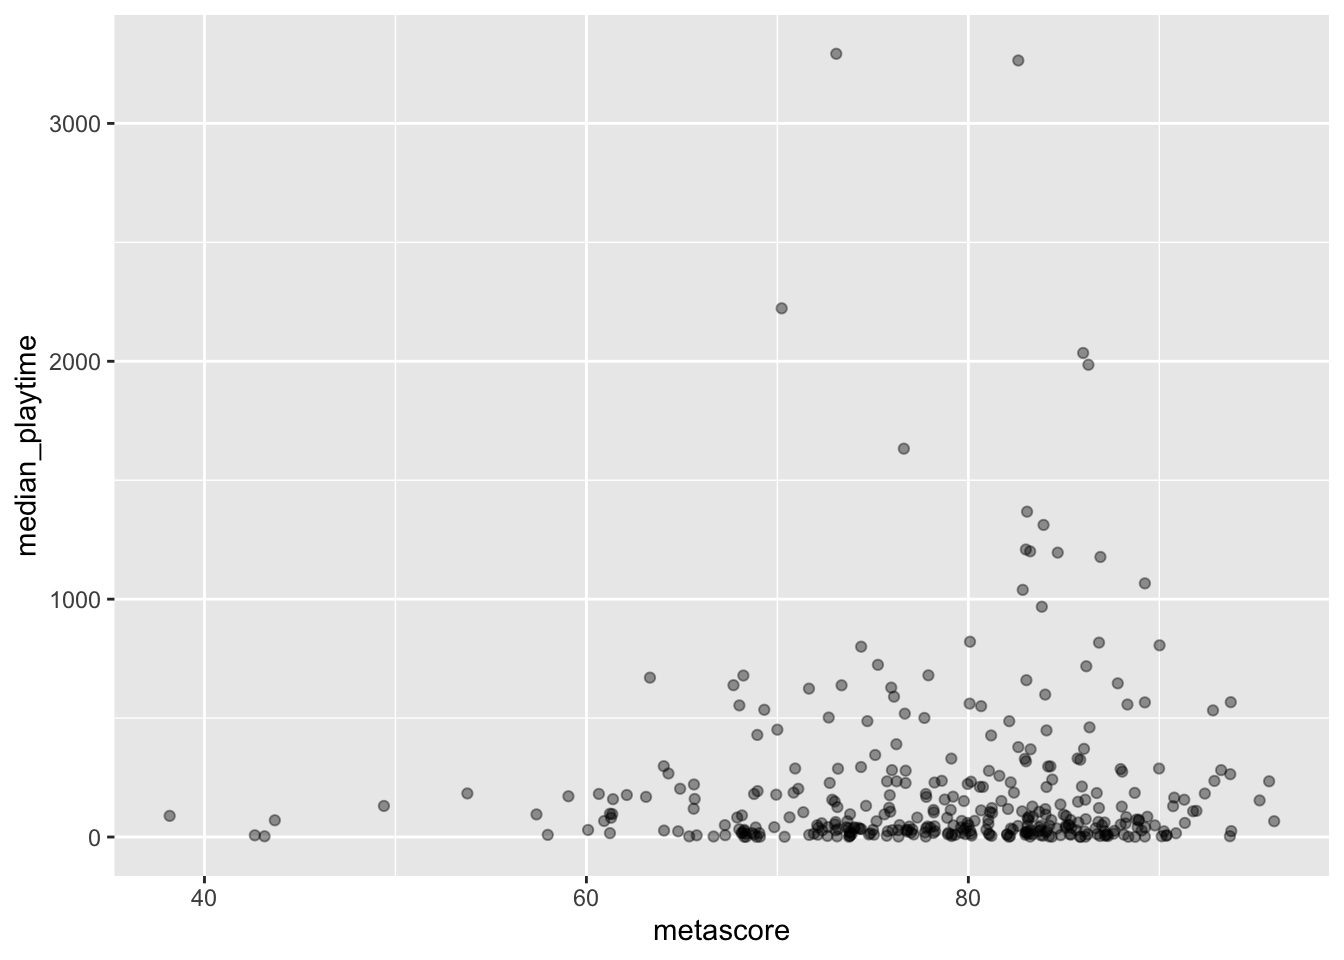
\includegraphics{03-dplyr_files/figure-latex/unnamed-chunk-49-1.pdf}

\begin{enumerate}
\def\labelenumi{\arabic{enumi}.}
\setcounter{enumi}{3}
\tightlist
\item
  * In some cases throughout this chapter, we've renamed data sets using \texttt{\textless{}-} with the same name like
\end{enumerate}

\begin{Shaded}
\begin{Highlighting}[]
\NormalTok{toy\_df }\OtherTok{\textless{}{-}}\NormalTok{ toy\_df }\SpecialCharTok{\%\textgreater{}\%} \FunctionTok{mutate}\NormalTok{(}\AttributeTok{newvar =}\NormalTok{ x }\SpecialCharTok{/}\NormalTok{ y)}
\end{Highlighting}
\end{Shaded}

In other cases, we've given the data set a new name, like

\begin{Shaded}
\begin{Highlighting}[]
\NormalTok{toy\_small }\OtherTok{\textless{}{-}}\NormalTok{ toy\_df }\SpecialCharTok{\%\textgreater{}\%} \FunctionTok{filter}\NormalTok{(}\SpecialCharTok{!}\FunctionTok{is.na}\NormalTok{(x))}
\end{Highlighting}
\end{Shaded}

For which of the functions below is a generally ``safe'' to name the data set using the same name after using the function. Why?

\begin{enumerate}
\def\labelenumi{\alph{enumi}.}
\tightlist
\item
  \texttt{mutate()}
\end{enumerate}

Usually fine: mutating creates a new variable, which doesn't change any of the other variables in the data set, if things get messed up with the new variable.

\begin{enumerate}
\def\labelenumi{\alph{enumi}.}
\setcounter{enumi}{1}
\tightlist
\item
  \texttt{arrange()}
\end{enumerate}

Usually fine: ordering the rows a certain way won't change any plots and doesn't change any of the underlying data.

\begin{enumerate}
\def\labelenumi{\alph{enumi}.}
\setcounter{enumi}{2}
\tightlist
\item
  \texttt{filter()}
\end{enumerate}

Usually not the best practice. Naming the data set the same name after the filter means that you permanently lose data that you filtered out, unless you re-read in the data set at the beginning.

\begin{enumerate}
\def\labelenumi{\alph{enumi}.}
\setcounter{enumi}{3}
\tightlist
\item
  \texttt{summarise()}
\end{enumerate}

Usually not the best practice. Again, naming the summarized data set the same as the original data means that you lose the original data, unless you re-read it in at the beginning. For example,

\begin{Shaded}
\begin{Highlighting}[]
\NormalTok{toy\_df }\OtherTok{\textless{}{-}}\NormalTok{ toy\_df }\SpecialCharTok{\%\textgreater{}\%} \FunctionTok{summarise}\NormalTok{(}\AttributeTok{meanx =} \FunctionTok{mean}\NormalTok{(x))}
\NormalTok{toy\_df}
\CommentTok{\#\textgreater{} \# A tibble: 1 x 1}
\CommentTok{\#\textgreater{}   meanx}
\CommentTok{\#\textgreater{}   \textless{}dbl\textgreater{}}
\CommentTok{\#\textgreater{} 1    NA}
\end{Highlighting}
\end{Shaded}

means that we now have no way to access the original data in \texttt{toy\_df}.

\begin{enumerate}
\def\labelenumi{\alph{enumi}.}
\setcounter{enumi}{4}
\tightlist
\item
  \texttt{select()}
\end{enumerate}

This can sometimes be okay if you're sure that the variables you are removing won't ever be used.

\hypertarget{rcode-3}{%
\section{\texorpdfstring{Non-Exercise \texttt{R} Code}{Non-Exercise R Code}}\label{rcode-3}}

\begin{Shaded}
\begin{Highlighting}[]
\FunctionTok{library}\NormalTok{(babynames)}
\FunctionTok{head}\NormalTok{(babynames)}
\FunctionTok{library}\NormalTok{(tidyverse)}
\NormalTok{slumajors\_df }\OtherTok{\textless{}{-}} \FunctionTok{read\_csv}\NormalTok{(}\StringTok{"data/SLU\_Majors\_15\_19.csv"}\NormalTok{)}
\NormalTok{slumajors\_df}
\NormalTok{slumajors\_df }\SpecialCharTok{\%\textgreater{}\%} \FunctionTok{mutate}\NormalTok{(}\AttributeTok{ntotal =}\NormalTok{ nfemales }\SpecialCharTok{+}\NormalTok{ nmales)}
\NormalTok{slumajors\_df }\SpecialCharTok{\%\textgreater{}\%}
  \FunctionTok{mutate}\NormalTok{(}\AttributeTok{percfemale =} \DecValTok{100} \SpecialCharTok{*}\NormalTok{ nfemales }\SpecialCharTok{/}\NormalTok{ (nfemales }\SpecialCharTok{+}\NormalTok{ nmales))}
\NormalTok{slumajors\_df }\OtherTok{\textless{}{-}}\NormalTok{ slumajors\_df }\SpecialCharTok{\%\textgreater{}\%}
  \FunctionTok{mutate}\NormalTok{(}\AttributeTok{percfemale =} \DecValTok{100} \SpecialCharTok{*}\NormalTok{ nfemales }\SpecialCharTok{/}\NormalTok{ (nfemales }\SpecialCharTok{+}\NormalTok{ nmales))}
\NormalTok{slumajors\_df }\OtherTok{\textless{}{-}}\NormalTok{ slumajors\_df }\SpecialCharTok{\%\textgreater{}\%} \FunctionTok{mutate}\NormalTok{(}\AttributeTok{ntotal =}\NormalTok{ nfemales }\SpecialCharTok{+}\NormalTok{ nmales)}
\NormalTok{slumajors\_df }\OtherTok{\textless{}{-}}\NormalTok{ slumajors\_df }\SpecialCharTok{\%\textgreater{}\%}
  \FunctionTok{mutate}\NormalTok{(}\AttributeTok{ntotal =}\NormalTok{ nfemales }\SpecialCharTok{+}\NormalTok{ nmales) }\SpecialCharTok{\%\textgreater{}\%}
  \FunctionTok{mutate}\NormalTok{(}\AttributeTok{percfemale =} \DecValTok{100} \SpecialCharTok{*}\NormalTok{ nfemales }\SpecialCharTok{/}\NormalTok{ (nfemales }\SpecialCharTok{+}\NormalTok{ nmales))}
\FunctionTok{mutate}\NormalTok{(}\FunctionTok{mutate}\NormalTok{(slumajors\_df, }\AttributeTok{ntotal =}\NormalTok{ nfemales }\SpecialCharTok{+}\NormalTok{ nmales), }\AttributeTok{percfemale =} \DecValTok{100} \SpecialCharTok{*}\NormalTok{ nfemales }\SpecialCharTok{/}\NormalTok{ (nfemales }\SpecialCharTok{+}\NormalTok{ nmales))}
\NormalTok{slumajors\_df }\SpecialCharTok{\%\textgreater{}\%} \FunctionTok{mutate}\NormalTok{(}\AttributeTok{morewomen =} \FunctionTok{if\_else}\NormalTok{(percfemale }\SpecialCharTok{\textgreater{}} \DecValTok{50}\NormalTok{,}
                                            \AttributeTok{true =} \StringTok{"Yes"}\NormalTok{,}
                                            \AttributeTok{false =} \StringTok{"No"}\NormalTok{))}
\NormalTok{slumajors\_df }\SpecialCharTok{\%\textgreater{}\%} \FunctionTok{mutate}\NormalTok{(}\AttributeTok{large\_majority =}
                          \FunctionTok{case\_when}\NormalTok{(percfemale }\SpecialCharTok{\textgreater{}=} \DecValTok{70} \SpecialCharTok{\textasciitilde{}} \StringTok{"female"}\NormalTok{,}
\NormalTok{                                    percfemale }\SpecialCharTok{\textless{}=} \DecValTok{30} \SpecialCharTok{\textasciitilde{}} \StringTok{"male"}\NormalTok{,}
\NormalTok{                                    percfemale }\SpecialCharTok{\textgreater{}} \DecValTok{30} \SpecialCharTok{\&}\NormalTok{ percfemale }\SpecialCharTok{\textless{}} \DecValTok{70} \SpecialCharTok{\textasciitilde{}} \StringTok{"none"}\NormalTok{)) }
\NormalTok{slumajors\_df }\OtherTok{\textless{}{-}}\NormalTok{ slumajors\_df }\SpecialCharTok{\%\textgreater{}\%}
  \FunctionTok{mutate}\NormalTok{(}\AttributeTok{morewomen =} \FunctionTok{if\_else}\NormalTok{(percfemale }\SpecialCharTok{\textgreater{}} \DecValTok{50}\NormalTok{,}
                             \AttributeTok{true =} \StringTok{"Yes"}\NormalTok{,}
                             \AttributeTok{false =} \StringTok{"No"}\NormalTok{)) }\SpecialCharTok{\%\textgreater{}\%}
  \FunctionTok{mutate}\NormalTok{(}\AttributeTok{large\_majority =}
           \FunctionTok{case\_when}\NormalTok{(percfemale }\SpecialCharTok{\textgreater{}=} \DecValTok{70} \SpecialCharTok{\textasciitilde{}} \StringTok{"female"}\NormalTok{,}
\NormalTok{                     percfemale }\SpecialCharTok{\textless{}=} \DecValTok{30} \SpecialCharTok{\textasciitilde{}} \StringTok{"male"}\NormalTok{,}
\NormalTok{                     percfemale }\SpecialCharTok{\textgreater{}} \DecValTok{30} \SpecialCharTok{\&}\NormalTok{ percfemale }\SpecialCharTok{\textless{}} \DecValTok{70} \SpecialCharTok{\textasciitilde{}} \StringTok{"none"}\NormalTok{)) }
\NormalTok{slumajors\_df }\SpecialCharTok{\%\textgreater{}\%} \FunctionTok{arrange}\NormalTok{(percfemale)}
\NormalTok{slumajors\_df }\SpecialCharTok{\%\textgreater{}\%} \FunctionTok{arrange}\NormalTok{(}\FunctionTok{desc}\NormalTok{(percfemale))}
\NormalTok{slumajors\_df }\SpecialCharTok{\%\textgreater{}\%} \FunctionTok{select}\NormalTok{(Major, ntotal)}
\NormalTok{slumajors\_df }\SpecialCharTok{\%\textgreater{}\%} \FunctionTok{select}\NormalTok{(}\SpecialCharTok{{-}}\NormalTok{ntotal, }\SpecialCharTok{{-}}\NormalTok{nfemales, }\SpecialCharTok{{-}}\NormalTok{nmales)}
\NormalTok{slumajors\_df }\SpecialCharTok{\%\textgreater{}\%} \FunctionTok{mutate}\NormalTok{(}\AttributeTok{propfemale =}\NormalTok{ percfemale }\SpecialCharTok{/} \DecValTok{100}\NormalTok{) }\SpecialCharTok{\%\textgreater{}\%}
  \FunctionTok{select}\NormalTok{(propfemale, }\FunctionTok{everything}\NormalTok{())}
\NormalTok{slumajors\_df }\SpecialCharTok{\%\textgreater{}\%} \FunctionTok{arrange}\NormalTok{(}\FunctionTok{desc}\NormalTok{(ntotal)) }\SpecialCharTok{\%\textgreater{}\%}
  \FunctionTok{slice}\NormalTok{(}\DecValTok{1}\NormalTok{, }\DecValTok{2}\NormalTok{, }\DecValTok{3}\NormalTok{, }\DecValTok{4}\NormalTok{, }\DecValTok{5}\NormalTok{)}
\FunctionTok{library}\NormalTok{(babynames)}
\NormalTok{babynames}
\NormalTok{babynames }\SpecialCharTok{\%\textgreater{}\%} \FunctionTok{filter}\NormalTok{(name }\SpecialCharTok{==} \StringTok{"Matthew"}\NormalTok{)}
\NormalTok{babynames }\SpecialCharTok{\%\textgreater{}\%} \FunctionTok{filter}\NormalTok{(year }\SpecialCharTok{\textgreater{}=} \DecValTok{2000}\NormalTok{)}
\NormalTok{babynames }\SpecialCharTok{\%\textgreater{}\%} \FunctionTok{filter}\NormalTok{(sex }\SpecialCharTok{!=} \StringTok{"M"}\NormalTok{)}
\NormalTok{babynames }\SpecialCharTok{\%\textgreater{}\%} \FunctionTok{filter}\NormalTok{(prop }\SpecialCharTok{\textgreater{}} \FloatTok{0.05}\NormalTok{)}
\NormalTok{babynames }\SpecialCharTok{\%\textgreater{}\%} \FunctionTok{filter}\NormalTok{(year }\SpecialCharTok{==} \FunctionTok{max}\NormalTok{(year))}
\NormalTok{babynames }\SpecialCharTok{\%\textgreater{}\%} \FunctionTok{filter}\NormalTok{(n }\SpecialCharTok{\textgreater{}} \DecValTok{20000} \SpecialCharTok{|}\NormalTok{ prop }\SpecialCharTok{\textgreater{}} \FloatTok{0.05}\NormalTok{)}
\NormalTok{babynames }\SpecialCharTok{\%\textgreater{}\%} \FunctionTok{filter}\NormalTok{(sex }\SpecialCharTok{==} \StringTok{"F"} \SpecialCharTok{\&}\NormalTok{ name }\SpecialCharTok{==} \StringTok{"Mary"}\NormalTok{)}
\NormalTok{babynames }\SpecialCharTok{\%\textgreater{}\%} \FunctionTok{filter}\NormalTok{(sex }\SpecialCharTok{==} \StringTok{"F"} \SpecialCharTok{\&}\NormalTok{ name }\SpecialCharTok{==} \StringTok{"Mary"} \SpecialCharTok{\&}\NormalTok{ prop }\SpecialCharTok{\textgreater{}} \FloatTok{0.05}\NormalTok{)}
\NormalTok{slumajors\_df }\SpecialCharTok{\%\textgreater{}\%}
  \FunctionTok{summarise}\NormalTok{(}\AttributeTok{meantotalmajor =} \FunctionTok{mean}\NormalTok{(ntotal),}
            \AttributeTok{totalgrad =} \FunctionTok{sum}\NormalTok{(ntotal))}
\NormalTok{babynames }\SpecialCharTok{\%\textgreater{}\%} \FunctionTok{group\_by}\NormalTok{(year) }\SpecialCharTok{\%\textgreater{}\%}
  \FunctionTok{summarise}\NormalTok{(}\AttributeTok{totalbirths =} \FunctionTok{sum}\NormalTok{(n))}
\NormalTok{babynames }\SpecialCharTok{\%\textgreater{}\%} \FunctionTok{summarise}\NormalTok{(}\AttributeTok{totalobs =} \FunctionTok{n}\NormalTok{())}
\NormalTok{babynames }\SpecialCharTok{\%\textgreater{}\%} \FunctionTok{group\_by}\NormalTok{(year) }\SpecialCharTok{\%\textgreater{}\%}
  \FunctionTok{summarise}\NormalTok{(}\AttributeTok{ngroup =} \FunctionTok{n}\NormalTok{())}
\NormalTok{toy\_df }\SpecialCharTok{\%\textgreater{}\%} \FunctionTok{summarise}\NormalTok{(}\AttributeTok{meanx =} \FunctionTok{mean}\NormalTok{(x, }\AttributeTok{na.rm =} \ConstantTok{TRUE}\NormalTok{))}
\NormalTok{toy\_df }\SpecialCharTok{\%\textgreater{}\%} \FunctionTok{mutate}\NormalTok{(}\AttributeTok{missingx =} \FunctionTok{is.na}\NormalTok{(x))}
\NormalTok{toy\_df }\SpecialCharTok{\%\textgreater{}\%} \FunctionTok{filter}\NormalTok{(}\FunctionTok{is.na}\NormalTok{(x) }\SpecialCharTok{!=} \ConstantTok{TRUE}\NormalTok{)}
\NormalTok{toy\_df }\SpecialCharTok{\%\textgreater{}\%} \FunctionTok{filter}\NormalTok{(}\SpecialCharTok{!}\FunctionTok{is.na}\NormalTok{(x))}
\end{Highlighting}
\end{Shaded}


  \bibliography{book.bib,packages.bib}

\end{document}
